\subsection{\pkg{Quizzipedia::Client}}
Racchiude tutte le componenti necessarie per il front-end del prodotto. Visualizza i dati dell'utente e invia richieste al server che dovrà gestirle e reindirizzare una risposta al client.
\begin{figure}[H]
\centering
\noindent\makebox[\textwidth]{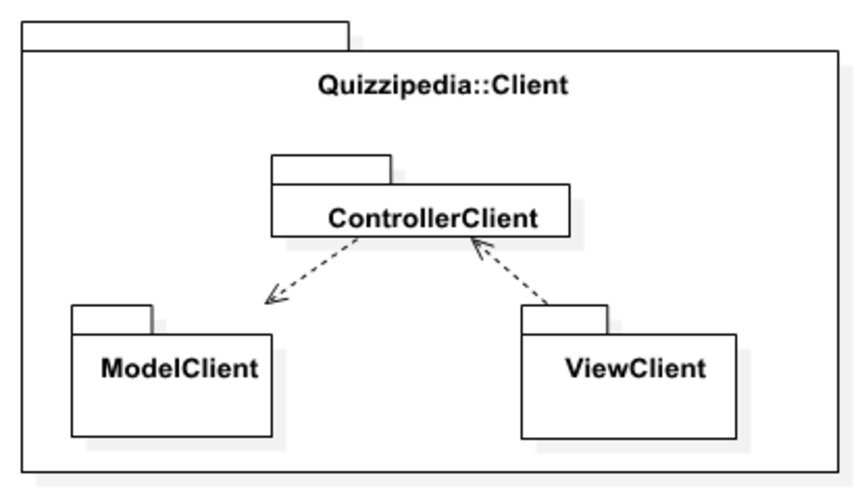
\includegraphics[width=\textwidth]{Img/quizzipedia-client.pdf}}
\caption[Schema Componente Client]{Schema Componente Quizzipedia::Client}
\end{figure}
\subsection{\pkg{Quizzipedia::Client::ModelClient}}
Rappresenta il modello dei dati che verranno utilizzati dal sistema lato client. Viene utilizzato tale model per facilitare il recupero di alcune informazioni che altrimenti dovrebbero esser recuperate dal server ogni volta che viene svolta una richiesta dall'utente.
Attraverso l'uso di Angular.js il controller svolge automaticamente le modifiche richieste dalla view nel model in modo tale da tenerlo sempre aggiornato.
\begin{figure}[H]
\centering
\noindent\makebox[\textwidth]{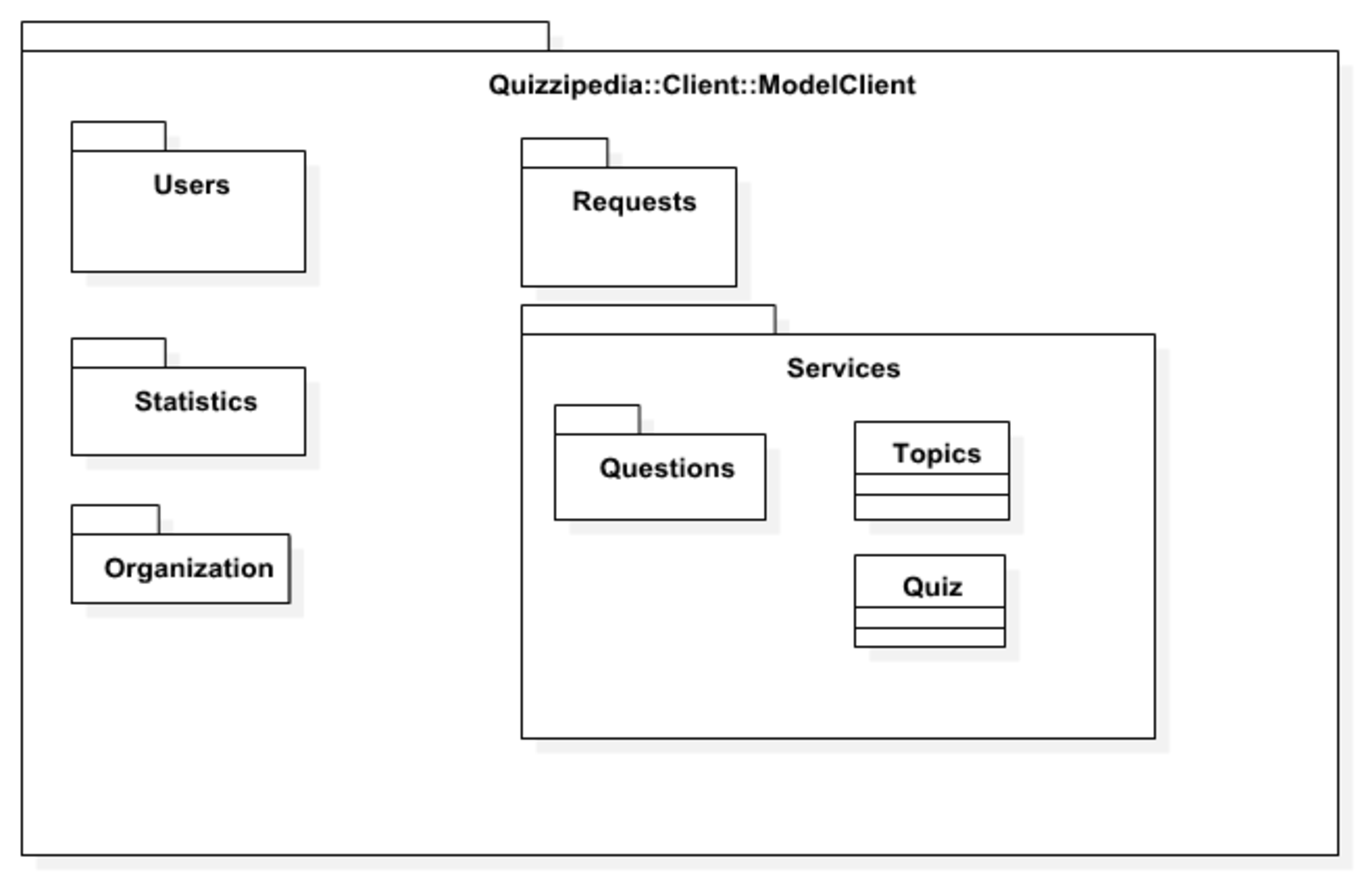
\includegraphics[width=\textwidth]{Img/quizzipedia-client-modelclient.pdf}}
\caption[Schema Componente Quizzipedia::Client::ModelClient]{Schema Componente Quizzipedia::Client::ModelClient}
\end{figure}
\subsubsection{Componenti contenute}
\begin{itemize}
\item \pkg{Quizzipedia::Client::ModelClient::Organizations}
\item \pkg{Quizzipedia::Client::ModelClient::Requests}
\item \pkg{Quizzipedia::Client::ModelClient::Services}
\item \pkg{Quizzipedia::Client::ModelClient::Statistics}
\item \pkg{Quizzipedia::Client::ModelClient::Users}
\end{itemize}
\subsubsection{Interazioni con altre componenti}
\begin{itemize}
\item \bold{Entranti}
\begin{itemize}
\item usata da \pkg{Quizzipedia::Client::ViewModelClient} per aggiungi
\end{itemize}
\end{itemize}
\subsection{\pkg{Quizzipedia::Client::ModelClient::Organizations}}
La componente gestisce le classi e gli enti, ovvero il sistema in base a cui sono organizzati gli utenti nel sistema.
\begin{figure}[H]
\centering
\noindent\makebox[\textwidth]{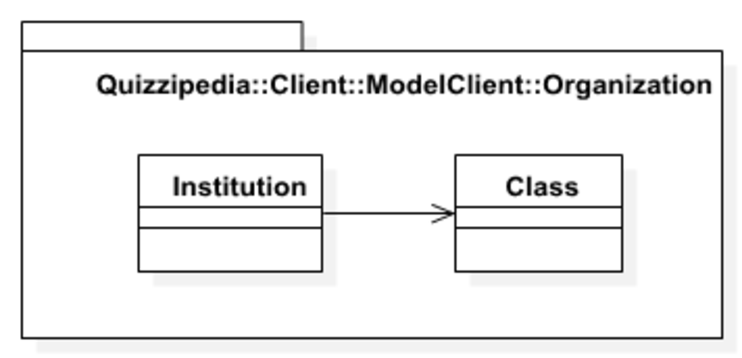
\includegraphics[width=\textwidth]{Img/quizzipedia-client-modelclient-organizations.pdf}}
\caption[Schema Componente Quizzipedia::Client::ModelClient::Organizations]{Schema Componente Quizzipedia::Client::ModelClient::Organizations}
\end{figure}
\subsubsection{Interazioni con altre componenti}
\begin{itemize}
\item \bold{Entranti}
\begin{itemize}
\item usata da \pkg{Quizzipedia::Client::ModelClient::Users} per organizzare gli utenti all'interno di enti e classi
\end{itemize}
\end{itemize}
\subsubsection{Classe \cls{Class}}
Rappresenta una classe all'interno di un ente. Memorizza le informazioni che definiscono ogni classe,
informazioni che saranno utilizzate per la visualizzazione e per la gestione della classe stessa.
\begin{figure}[H]
\centering
\noindent\makebox[\textwidth]{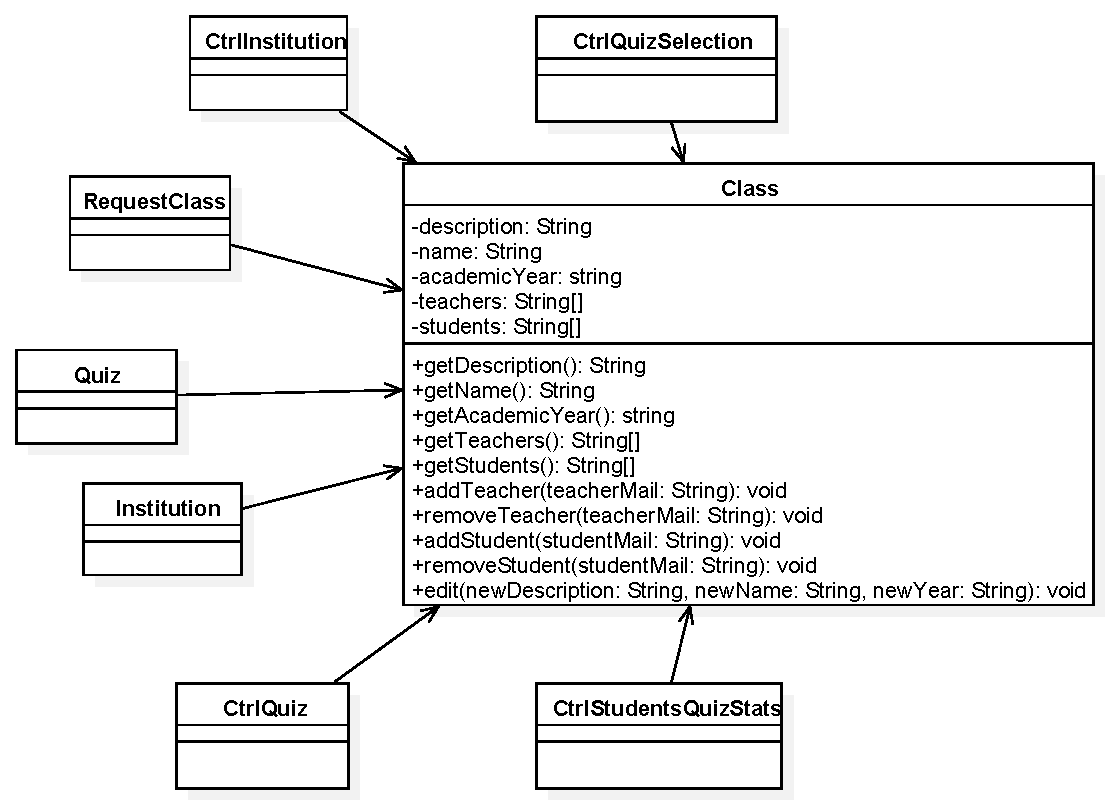
\includegraphics[width=\textwidth]{Img/quizzipedia-client-modelclient-organizations-class.pdf}}
\caption[Schema Classe Class]{Schema Classe Quizzipedia::Client::ModelClient::Organizations::Class}
\end{figure}
\paragraph{Relazioni con altre classi}
\subparagraph{Entranti}
\begin{itemize}
\item usata da \cls{Quizzipedia::Client::ModelClient::Organizations::Institution} per memorizzare la lista
delle classi presenti in un ente
\item usata da \cls{Quizzipedia::Client::ModelClient::Requests::RequestClass} per identificare la classe
in cui l'utente vuole essere inserito
\item usata da \cls{Quizzipedia::Client::ModelClient::Services::Quiz} per tenere traccia delle classi per
cui il quiz è stato creato. Se un quiz è assegnato a delle classi specifiche, allora è privato e
accessibile dai soli studenti delle classi
\item usata da \cls{Quizzipedia::Client::ModelClient::Users::User} per tenere traccia delle classi dell'ente
a cui l'utente è iscritto, o come docente, o come studente
\item usata da \cls{Quizzipedia::Client::ViewModelClient::CtrlOrganization::CtrlInstitution} per avere
accesso alla struttura della classe e potere quindi svolgere correttamente operazioni su di
essa
\end{itemize}
\subsubsection{Classe \cls{Institution}}
Tale classe rappresenta un ente. Contiene le informazioni relative alla struttura dell'ente che saranno visualizzate dall'utente e gestiste dal controller, come ad esempio la lista delle classi presenti nell'ente, la lista degli studenti e degli insegnati all'interno dell'ente.
\begin{figure}[H]
\centering
\noindent\makebox[\textwidth]{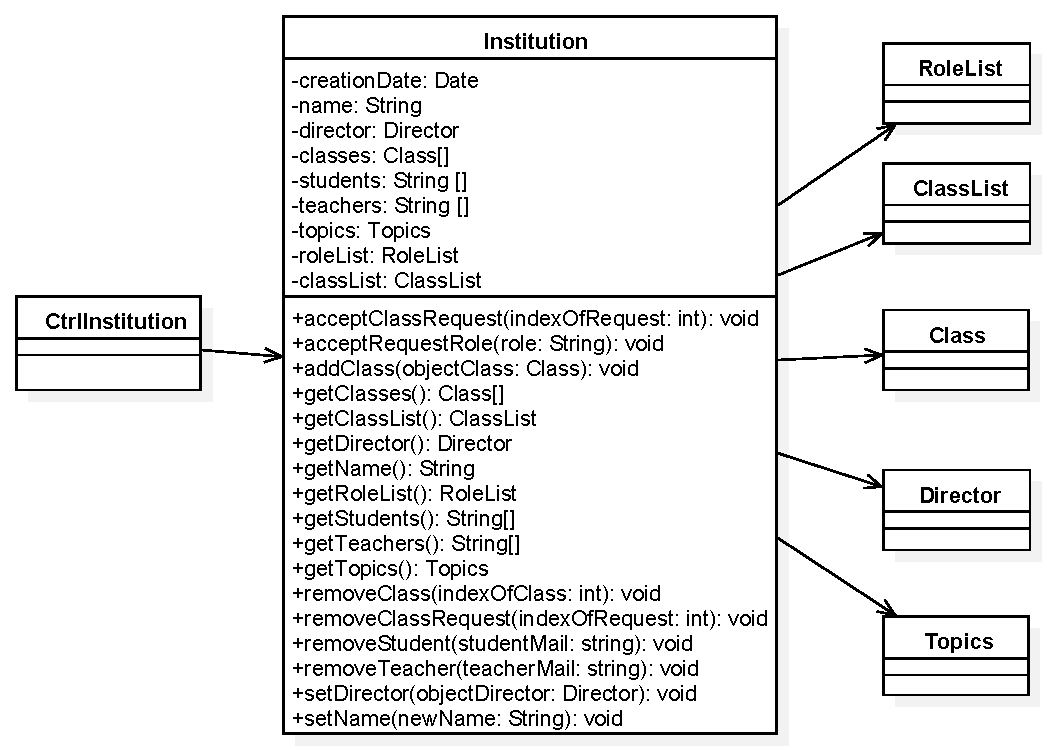
\includegraphics[width=\textwidth]{Img/quizzipedia-client-modelclient-organizations-institution.pdf}}
\caption[Schema Classe Institution]{Schema Classe Quizzipedia::Client::ModelClient::Organizations::Institution}
\end{figure}
\paragraph{Relazioni con altre classi}
\subparagraph{Entranti}
\begin{itemize}
\item usata da \cls{Quizzipedia::Client::ViewModelClient::CtrlOrganization::CtrlInstitution} per avere accesso alla struttura dell'istituto e caricare correttamente l'istituto corrente
\end{itemize}
\subparagraph{Uscenti}
\begin{itemize}
\item usa \cls{Quizzipedia::Client::ModelClient::Organizations::Class} per memorizzare la lista
delle classi presenti in un ente
\item usa \cls{Quizzipedia::Client::ModelClient::Requests::ClassList} per gestire la lista delle richieste di accesso a una delle proprie classi
\item usa \cls{Quizzipedia::Client::ModelClient::Requests::RoleList} per gestire la lista delle richieste di assegnazione di ruolo degli utenti
\end{itemize}
\subsection{\pkg{Quizzipedia::Client::ModelClient::Requests}}
Questo componente contiene le classi necessarie a gestire le richieste di ruolo e di classe degli utenti autenticati.
\begin{figure}[H]
\centering
\noindent\makebox[\textwidth]{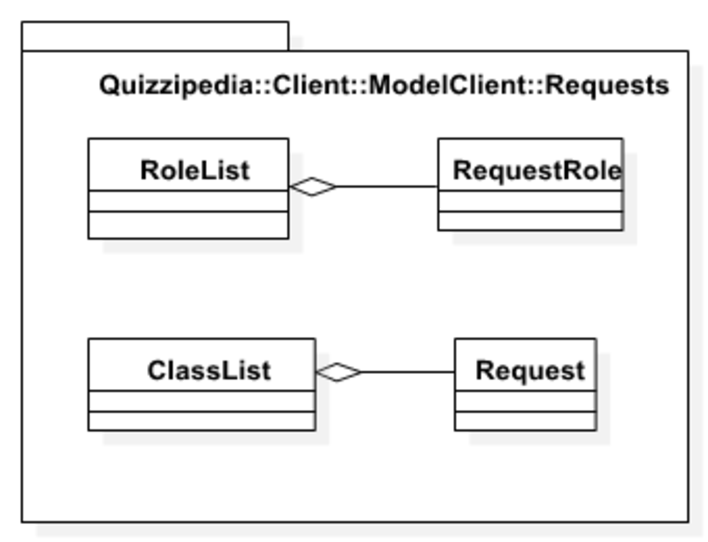
\includegraphics[width=\textwidth]{Img/quizzipedia-client-modelclient-requests.pdf}}
\caption[Schema Componente Quizzipedia::Client::ModelClient::Requests]{Schema Componente Quizzipedia::Client::ModelClient::Requests}
\end{figure}
\subsubsection{Interazioni con altre componenti}
\begin{itemize}
\item \bold{Entranti}
\begin{itemize}
\item usata da \pkg{Quizzipedia::Client::ModelClient::Users} per permettere agli utenti di effettuare richieste. Le richieste possono essere di ruolo o di classe
\end{itemize}
\end{itemize}
\subsubsection{Classe \cls{ClassList}}
Questa classe gestisce le richieste da parte di docenti o studenti per l'assegnazione a una specifica classe. Contiene i metodi da cui è possibile accettare o rifiutare la richiesta dell'utente.
\begin{figure}[H]
\centering
\noindent\makebox[\textwidth]{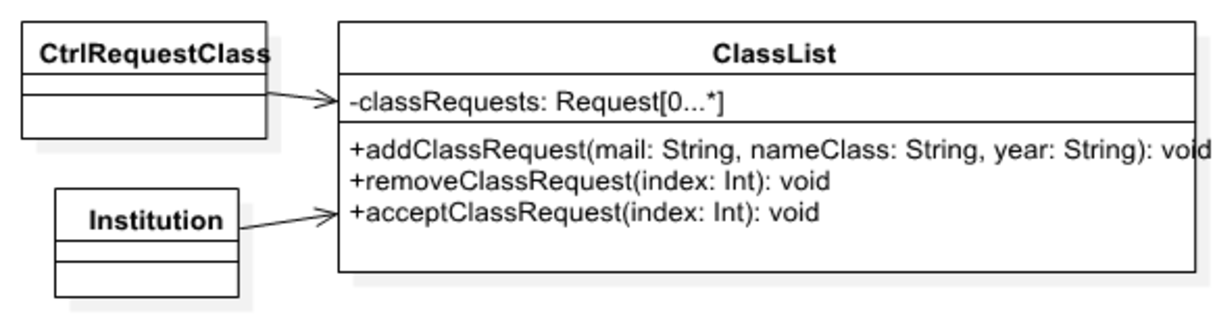
\includegraphics[width=\textwidth]{Img/quizzipedia-client-modelclient-requests-classlist.pdf}}
\caption[Schema Classe ClassList]{Schema Classe Quizzipedia::Client::ModelClient::Requests::ClassList}
\end{figure}
\paragraph{Relazioni con altre classi}
\subparagraph{Entranti}
\begin{itemize}
\item usata da \cls{Quizzipedia::Client::ModelClient::Organizations::Institution} per gestire la lista delle richieste di accesso a una delle proprie classi
\item usata da \cls{Quizzipedia::Client::ViewModelClient::CtrlRequests::CtrlRequestClass} per avere accesso alla lista di richieste e poterle gestire correttamente
\end{itemize}
\subparagraph{Uscenti}
\begin{itemize}
\item usa \cls{Quizzipedia::Client::ModelClient::Requests::RequestClass} per creare una lista in cui compaiano gli utenti e le classi in cui desiderano entrare
\end{itemize}
\subsubsection{Classe \cls{RequestClass}}
La classe memorizza l'utente che invia la richiesta di inserimento in una classe e la classe per cui la richiesta è stata effettuata.
\begin{figure}[H]
\centering
\noindent\makebox[\textwidth]{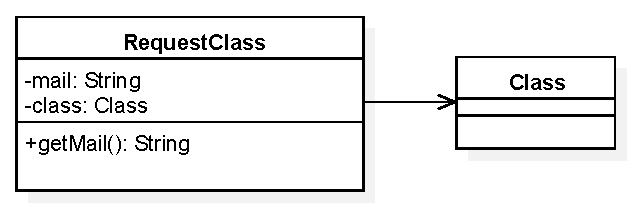
\includegraphics[width=\textwidth]{Img/quizzipedia-client-modelclient-requests-requestclass.pdf}}
\caption[Schema Classe RequestClass]{Schema Classe Quizzipedia::Client::ModelClient::Requests::RequestClass}
\end{figure}
\paragraph{Relazioni con altre classi}
\subparagraph{Entranti}
\begin{itemize}
\item usata da \cls{Quizzipedia::Client::ModelClient::Requests::ClassList} per creare una lista in cui compaiano gli utenti e le classi in cui desiderano entrare
\end{itemize}
\subparagraph{Uscenti}
\begin{itemize}
\item usa \cls{Quizzipedia::Client::ModelClient::Organizations::Class} per identificare la classe
in cui l'utente vuole essere inserito
\end{itemize}
\subsubsection{Classe \cls{RequestRole}}
La classe memorizza l'utente che invia una richiesta di ruolo e il ruolo che vuole ricoprire.
\begin{figure}[H]
\centering
\noindent\makebox[\textwidth]{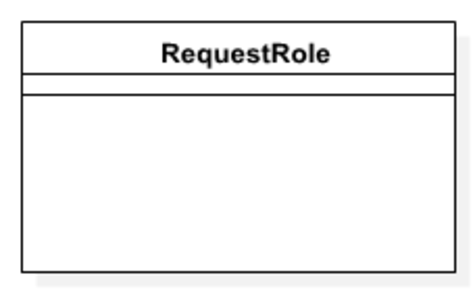
\includegraphics[width=\textwidth]{Img/quizzipedia-client-modelclient-requests-requestrole.pdf}}
\caption[Schema Classe RequestRole]{Schema Classe Quizzipedia::Client::ModelClient::Requests::RequestRole}
\end{figure}
\paragraph{Relazioni con altre classi}
\subparagraph{Entranti}
\begin{itemize}
\item usata da \cls{Quizzipedia::Client::ModelClient::Requests::RoleList} per memorizzare una lista delle richieste di ruolo degli utenti di un istituto
\end{itemize}
\subsubsection{Classe \cls{RoleList}}
Gli utenti senza ruolo inviano le proprie richieste per l'assegnazione al ruolo di studente o docente al responsabile di un ente. Questa classe gestisce tali richieste.
\begin{figure}[H]
\centering
\noindent\makebox[\textwidth]{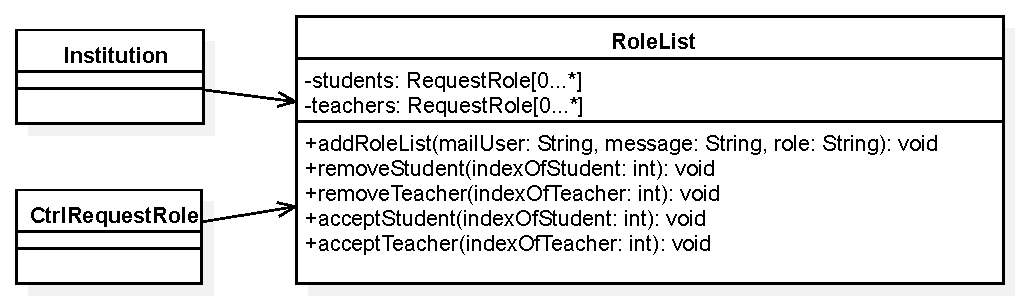
\includegraphics[width=\textwidth]{Img/quizzipedia-client-modelclient-requests-rolelist.pdf}}
\caption[Schema Classe RoleList]{Schema Classe Quizzipedia::Client::ModelClient::Requests::RoleList}
\end{figure}
\paragraph{Relazioni con altre classi}
\subparagraph{Entranti}
\begin{itemize}
\item usata da \cls{Quizzipedia::Client::ModelClient::Organizations::Institution} per gestire la lista delle richieste di assegnazione di ruolo degli utenti
\item usata da \cls{Quizzipedia::Client::ViewModelClient::CtrlRequests::CtrlRequestRole} per gestire le richieste di ruolo pendenti
\end{itemize}
\subparagraph{Uscenti}
\begin{itemize}
\item usa \cls{Quizzipedia::Client::ModelClient::Requests::RequestRole} per memorizzare una lista delle richieste di ruolo degli utenti di un istituto
\end{itemize}
\subsection{\pkg{Quizzipedia::Client::ModelClient::Services}}
Il componente racchiude i modelli necessari alla creazione di domande e quiz, i servizi principali offerti dal nostro prodotto.
\begin{figure}[H]
\centering
\noindent\makebox[\textwidth]{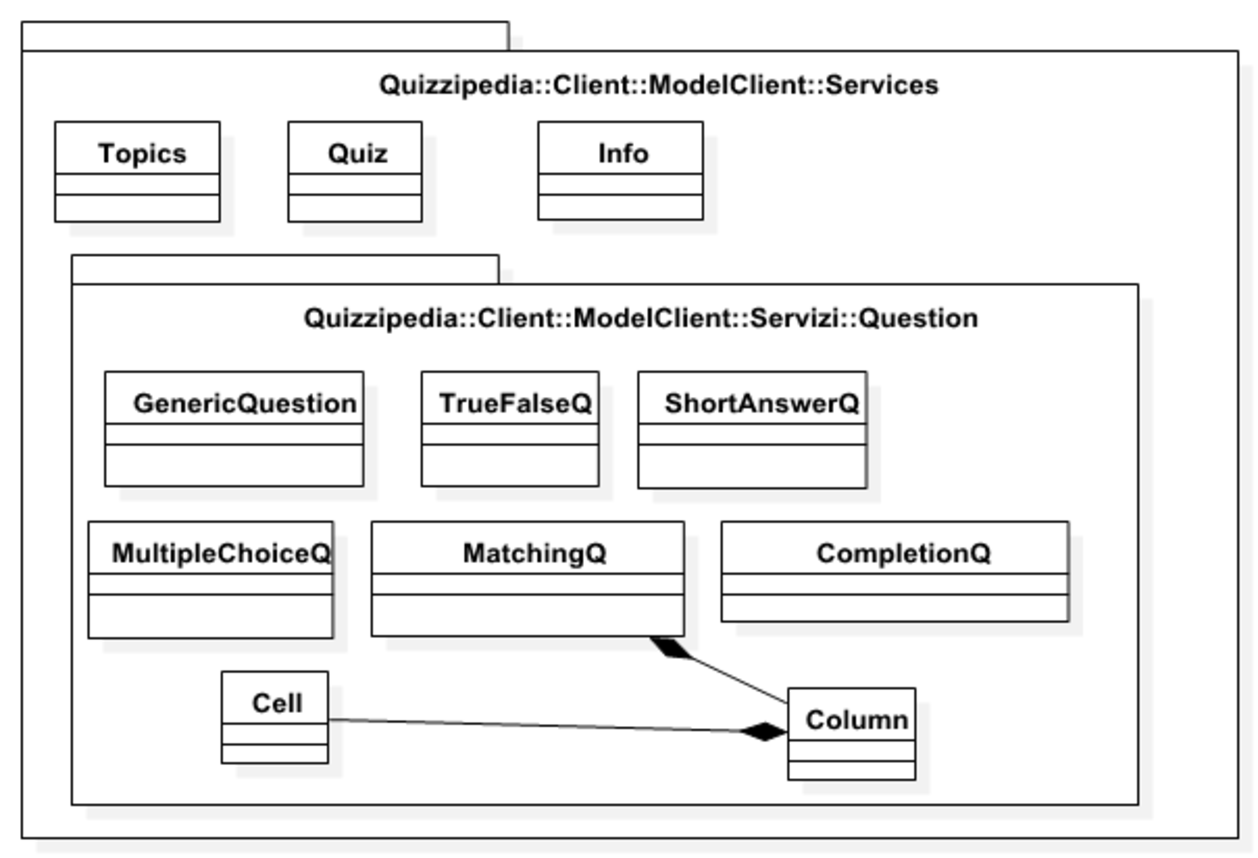
\includegraphics[width=\textwidth]{Img/quizzipedia-client-modelclient-services.pdf}}
\caption[Schema Componente Quizzipedia::Client::ModelClient::Services]{Schema Componente Quizzipedia::Client::ModelClient::Services}
\end{figure}
\subsubsection{Componenti contenute}
\begin{itemize}
\item \pkg{Quizzipedia::Client::ModelClient::Services::Answers}
\item \pkg{Quizzipedia::Client::ModelClient::Services::Questions}
\end{itemize}
\subsubsection{Interazioni con altre componenti}
\begin{itemize}
\item \bold{Entranti}
\begin{itemize}
\item usata da \pkg{Quizzipedia::Client::ModelClient::Users} per Permettere agli utenti di tenere traccia dello storico dei quiz svolti
\end{itemize}
\end{itemize}
\subsubsection{Classe \cls{Quiz}}
Include la struttura del quiz.
\begin{figure}[H]
\centering
\noindent\makebox[\textwidth]{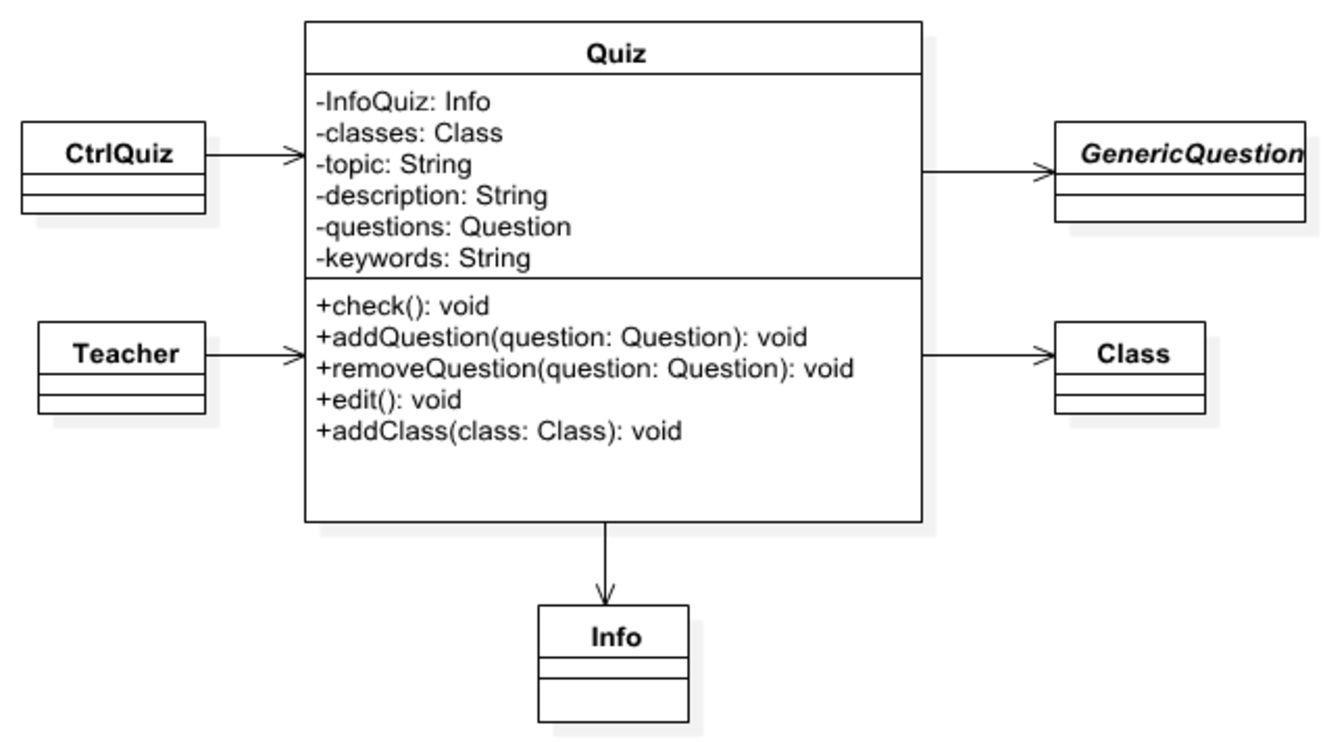
\includegraphics[width=\textwidth]{Img/quizzipedia-client-modelclient-services-quiz.pdf}}
\caption[Schema Classe Quiz]{Schema Classe Quizzipedia::Client::ModelClient::Services::Quiz}
\end{figure}
\paragraph{Relazioni con altre classi}
\subparagraph{Entranti}
\begin{itemize}
\item usata da \cls{Quizzipedia::Client::ModelClient::Users::Teacher} per aggiungi
\item usata da \cls{Quizzipedia::Client::ViewModelClient::CtrlServices::CtrlQuiz} per aggiungi
\end{itemize}
\subparagraph{Uscenti}
\begin{itemize}
\item usa \cls{Quizzipedia::Client::ModelClient::Organizations::Class} per tenere traccia delle classi per
cui il quiz è stato creato. Se un quiz è assegnato a delle classi specifiche, allora è privato e
accessibile dai soli studenti delle classi
\item usa \cls{Quizzipedia::Client::ModelClient::Services::Questions::GenericQuestion} per aggiungi
\end{itemize}
\subsubsection{Classe \cls{Topics}}
Modella la struttura necessaria a memorizzare la lista di argomenti. A ogni domanda e a ogni quiz verranno poi associati i relativi argomenti .
\begin{figure}[H]
\centering
\noindent\makebox[\textwidth]{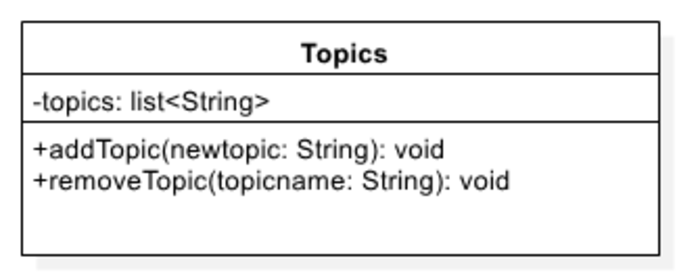
\includegraphics[width=\textwidth]{Img/quizzipedia-client-modelclient-services-topics.pdf}}
\caption[Schema Classe Topics]{Schema Classe Quizzipedia::Client::ModelClient::Services::Topics}
\end{figure}
\paragraph{Relazioni con altre classi}
\subparagraph{Entranti}
\begin{itemize}
\item usata da \cls{Quizzipedia::Client::ModelClient::Users::Director} per permettere al responsabile di modificare la lista dei possibili argomenti
\end{itemize}
\subsection{\pkg{Quizzipedia::Client::ModelClient::Services::Answers}}
Raccoglie tutte le componenti necessarie alla gestione della verifica dei quiz e delle domande svolte.
\begin{figure}[H]
\centering
\noindent\makebox[\textwidth]{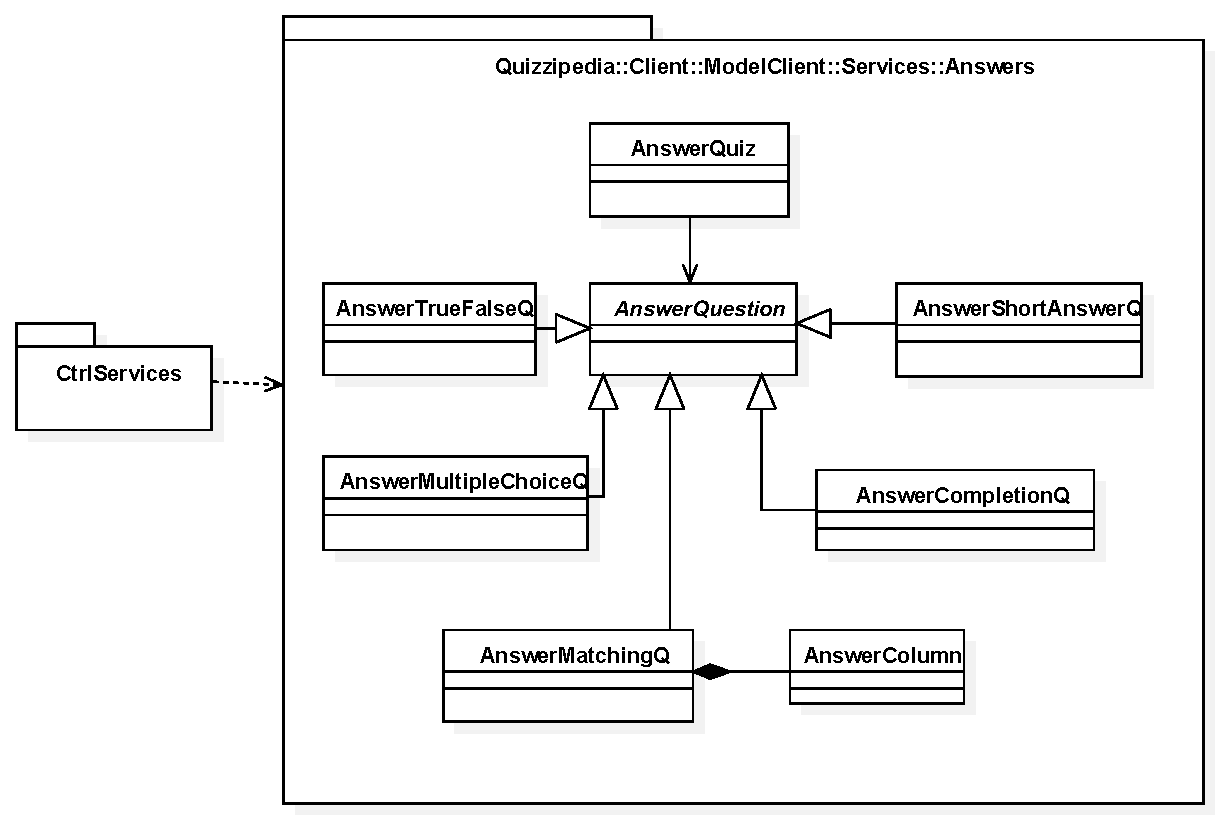
\includegraphics[width=\textwidth]{Img/quizzipedia-client-modelclient-services-answers.pdf}}
\caption[Schema Componente Quizzipedia::Client::ModelClient::Services::Answers]{Schema Componente Quizzipedia::Client::ModelClient::Services::Answers}
\end{figure}
\subsubsection{Interazioni con altre componenti}
\begin{itemize}
\item \bold{Uscenti}
\begin{itemize}
\item usa \pkg{Quizzipedia::Client::ModelClient::Services::Questions} per associare le risposte date dall'utente alla domanda giusta
\end{itemize}
\end{itemize}
\subsubsection{Classe \cls{AnswerColumn}}
Classe utilizzata da AnswerMatchingQ per salvare le risposte della domanda MatchingQ.
\begin{figure}[H]
\centering
\noindent\makebox[\textwidth]{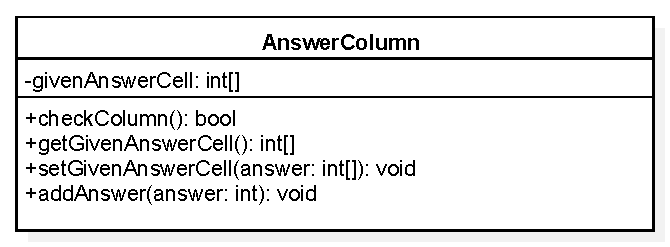
\includegraphics[width=\textwidth]{Img/quizzipedia-client-modelclient-services-answers-answercolumn.pdf}}
\caption[Schema Classe AnswerColumn]{Schema Classe Quizzipedia::Client::ModelClient::Services::Answers::AnswerColumn}
\end{figure}
\subsubsection{Classe \cls{AnswerCompletionQ}}
Classe che si occupa di memorizzare le informazioni di un domanda CompletionQ risolta.
\begin{figure}[H]
\centering
\noindent\makebox[\textwidth]{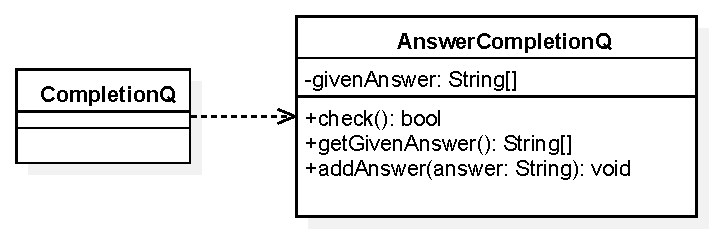
\includegraphics[width=\textwidth]{Img/quizzipedia-client-modelclient-services-answers-answercompletionq.pdf}}
\caption[Schema Classe AnswerCompletionQ]{Schema Classe Quizzipedia::Client::ModelClient::Services::Answers::AnswerCompletionQ}
\end{figure}
\paragraph{Relazioni con altre classi}
\subparagraph{Uscenti}
\begin{itemize}
\item usa \cls{Quizzipedia::Client::ModelClient::Services::Answers::AnswerQuestion} per concretizzarla, ereditandone così i campi dati e i metodi concreti. Inoltre, la classe concretizza il metodo check e memorizza correttamente la risposta data in caso di risposta a domanda a completamento
\end{itemize}
\subsubsection{Classe \cls{AnswerMatchingQ}}
Classe che si occupa di memorizzare le informazioni di un domanda MatchingQ risolta.
\begin{figure}[H]
\centering
\noindent\makebox[\textwidth]{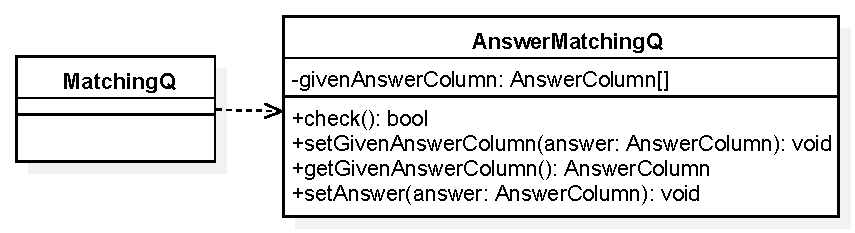
\includegraphics[width=\textwidth]{Img/quizzipedia-client-modelclient-services-answers-answermatchingq.pdf}}
\caption[Schema Classe AnswerMatchingQ]{Schema Classe Quizzipedia::Client::ModelClient::Services::Answers::AnswerMatchingQ}
\end{figure}
\subsubsection{Classe \cls{AnswerMultipleChoiceQ}}
Classe che si occupa di memorizzare le informazioni di un domanda MultipleChoiceQ risolta.
\begin{figure}[H]
\centering
\noindent\makebox[\textwidth]{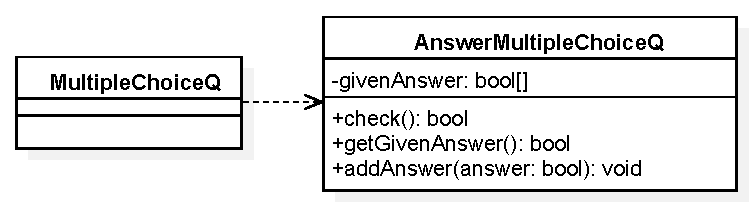
\includegraphics[width=\textwidth]{Img/quizzipedia-client-modelclient-services-answers-answermultiplechoiceq.pdf}}
\caption[Schema Classe AnswerMultipleChoiceQ]{Schema Classe Quizzipedia::Client::ModelClient::Services::Answers::AnswerMultipleChoiceQ}
\end{figure}
\paragraph{Relazioni con altre classi}
\subparagraph{Uscenti}
\begin{itemize}
\item usa \cls{Quizzipedia::Client::ModelClient::Services::Answers::AnswerQuestion} per concretizzarla, ereditandone così i campi dati e i metodi concreti. Inoltre, la classe concretizza il metodo check e memorizza correttamente la risposta data in caso di risposta a domanda a scelta multipla
\end{itemize}
\subsubsection{Classe \cls{AnswerQuestion}}
Classe che si occupa di memorizzare le informazioni di un domanda risolta.
\begin{figure}[H]
\centering
\noindent\makebox[\textwidth]{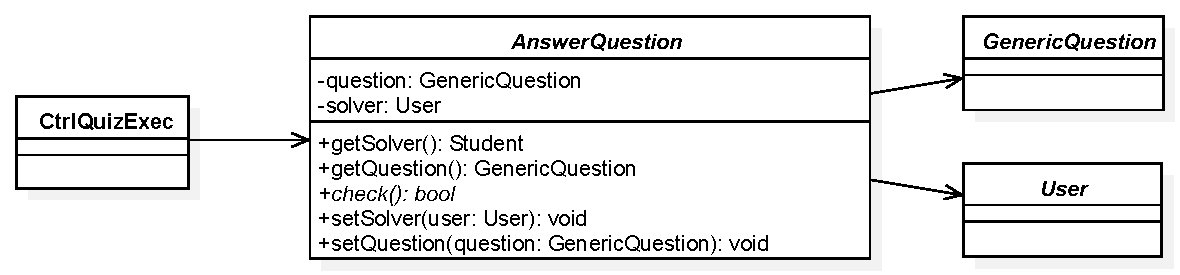
\includegraphics[width=\textwidth]{Img/quizzipedia-client-modelclient-services-answers-answerquestion.pdf}}
\caption[Schema Classe AnswerQuestion]{Schema Classe Quizzipedia::Client::ModelClient::Services::Answers::AnswerQuestion}
\end{figure}
\paragraph{Relazioni con altre classi}
\subparagraph{Entranti}
\begin{itemize}
\item usata da \cls{Quizzipedia::Client::ModelClient::Services::Answers::AnswerCompletionQ} per concretizzarla, ereditandone così i campi dati e i metodi concreti. Inoltre, la classe concretizza il metodo check e memorizza correttamente la risposta data in caso di risposta a domanda a completamento
\item usata da \cls{Quizzipedia::Client::ModelClient::Services::Answers::AnswerMultipleChoiceQ} per concretizzarla, ereditandone così i campi dati e i metodi concreti. Inoltre, la classe concretizza il metodo check e memorizza correttamente la risposta data in caso di risposta a domanda a scelta multipla
\item usata da \cls{Quizzipedia::Client::ModelClient::Services::Answers::AnswerShortAnswerQ} per concretizzarla, ereditandone così i campi dati e i metodi concreti. Inoltre, la classe concretizza il metodo check e memorizza correttamente la risposta data in caso di risposta a domanda aperta
\item usata da \cls{Quizzipedia::Client::ModelClient::Services::Answers::AnswerTrueFalseQ} per concretizzarla, ereditandone così i campi dati e i metodi concreti. Inoltre, la classe concretizza il metodo check e memorizza correttamente la risposta data in caso di risposta a domanda di tipo vero/falso
\end{itemize}
\subparagraph{Uscenti}
\begin{itemize}
\item usa \cls{Quizzipedia::Client::ModelClient::Services::Questions::GenericQuestion} per tenere traccia della domanda a cui corrisponde la risposta in questione
\item usa \cls{Quizzipedia::Client::ModelClient::Users::User} per tenere traccia di quale utente ha dato la risposta in questione
\end{itemize}
\subsubsection{Classe \cls{AnswerQuiz}}
Classe che si occupa di memorizzare le informazioni di un quiz completato e gestisce la verifica del suo superamento.
\begin{figure}[H]
\centering
\noindent\makebox[\textwidth]{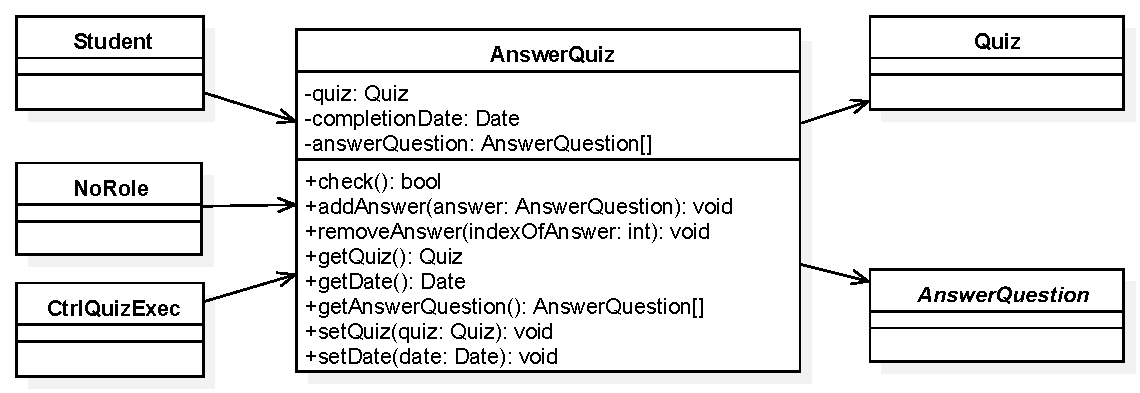
\includegraphics[width=\textwidth]{Img/quizzipedia-client-modelclient-services-answers-answerquiz.pdf}}
\caption[Schema Classe AnswerQuiz]{Schema Classe Quizzipedia::Client::ModelClient::Services::Answers::AnswerQuiz}
\end{figure}
\subsubsection{Classe \cls{AnswerShortAnswerQ}}
Classe che si occupa di memorizzare le informazioni di un domanda ShortAnswerQ risolta.
\begin{figure}[H]
\centering
\noindent\makebox[\textwidth]{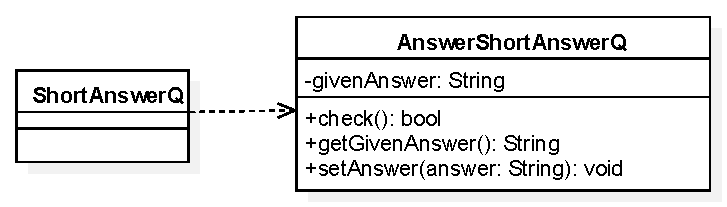
\includegraphics[width=\textwidth]{Img/quizzipedia-client-modelclient-services-answers-answershortanswerq.pdf}}
\caption[Schema Classe AnswerShortAnswerQ]{Schema Classe Quizzipedia::Client::ModelClient::Services::Answers::AnswerShortAnswerQ}
\end{figure}
\paragraph{Relazioni con altre classi}
\subparagraph{Uscenti}
\begin{itemize}
\item usa \cls{Quizzipedia::Client::ModelClient::Services::Answers::AnswerQuestion} per concretizzarla, ereditandone così i campi dati e i metodi concreti. Inoltre, la classe concretizza il metodo check e memorizza correttamente la risposta data in caso di risposta a domanda aperta
\end{itemize}
\subsubsection{Classe \cls{AnswerTrueFalseQ}}
Classe che si occupa di memorizzare le informazioni di un domanda TrueFalseQ risolta.
\begin{figure}[H]
\centering
\noindent\makebox[\textwidth]{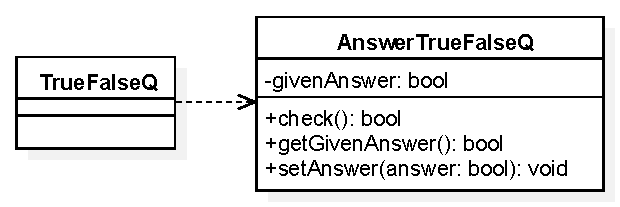
\includegraphics[width=\textwidth]{Img/quizzipedia-client-modelclient-services-answers-answertruefalseq.pdf}}
\caption[Schema Classe AnswerTrueFalseQ]{Schema Classe Quizzipedia::Client::ModelClient::Services::Answers::AnswerTrueFalseQ}
\end{figure}
\paragraph{Relazioni con altre classi}
\subparagraph{Uscenti}
\begin{itemize}
\item usa \cls{Quizzipedia::Client::ModelClient::Services::Answers::AnswerQuestion} per concretizzarla, ereditandone così i campi dati e i metodi concreti. Inoltre, la classe concretizza il metodo check e memorizza correttamente la risposta data in caso di risposta a domanda di tipo vero/falso
\end{itemize}
\subsection{\pkg{Quizzipedia::Client::ModelClient::Services::Questions}}
Descrive il modo in cui sono strutturati i vari tipi di domande che l'utente può incontrare durante la creazione o la compilazione di quiz.
\begin{figure}[H]
\centering
\noindent\makebox[\textwidth]{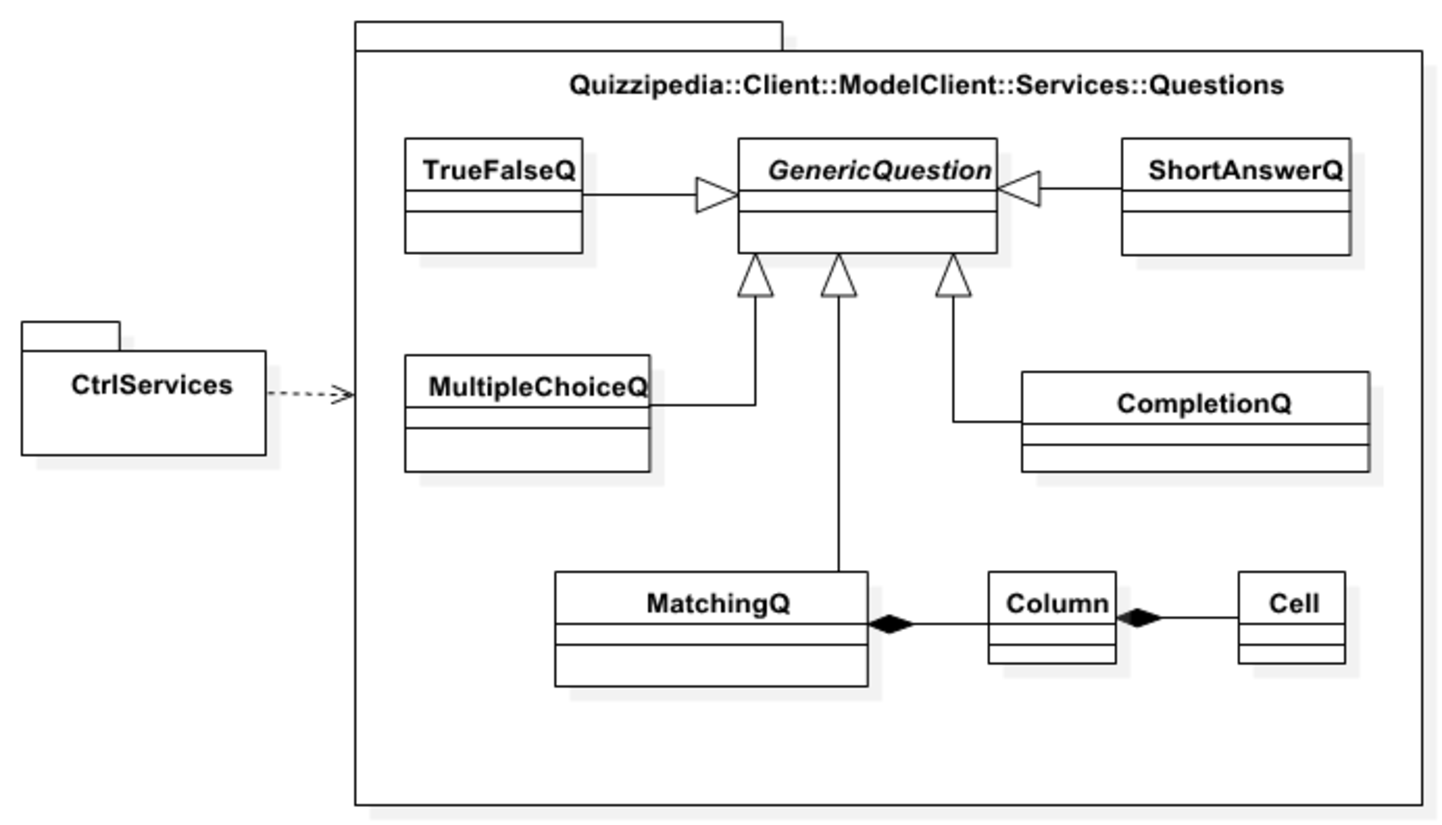
\includegraphics[width=\textwidth]{Img/quizzipedia-client-modelclient-services-questions.pdf}}
\caption[Schema Componente Quizzipedia::Client::ModelClient::Services::Questions]{Schema Componente Quizzipedia::Client::ModelClient::Services::Questions}
\end{figure}
\subsubsection{Interazioni con altre componenti}
\begin{itemize}
\item \bold{Entranti}
\begin{itemize}
\item usata da \pkg{Quizzipedia::Client::ModelClient::Services::Answers} per associare le risposte date dall'utente alla domanda giusta
\item usata da \pkg{Quizzipedia::Client::ViewModelClient::CtrlServices} per 
\end{itemize}
\end{itemize}
\subsubsection{Classe \cls{Cell}}
La classe descrive ogni singola riga (quindi ogni opzione) della colonna della domanda a collegamento.
\begin{figure}[H]
\centering
\noindent\makebox[\textwidth]{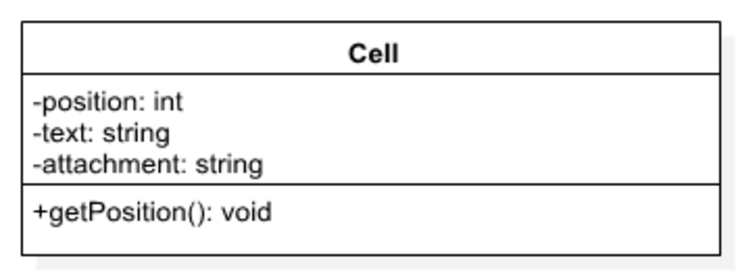
\includegraphics[width=\textwidth]{Img/quizzipedia-client-modelclient-services-questions-cell.pdf}}
\caption[Schema Classe Cell]{Schema Classe Quizzipedia::Client::ModelClient::Services::Questions::Cell}
\end{figure}
\paragraph{Relazioni con altre classi}
\subparagraph{Entranti}
\begin{itemize}
\item usata da \cls{Quizzipedia::Client::ModelClient::Services::Questions::Column} per aggiungi
\end{itemize}
\subsubsection{Classe \cls{Column}}
La classe descrive le colonne della domanda a collegamenti.
\begin{figure}[H]
\centering
\noindent\makebox[\textwidth]{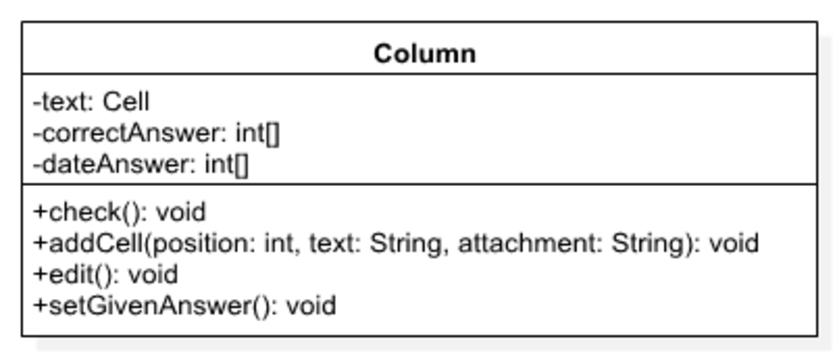
\includegraphics[width=\textwidth]{Img/quizzipedia-client-modelclient-services-questions-column.pdf}}
\caption[Schema Classe Column]{Schema Classe Quizzipedia::Client::ModelClient::Services::Questions::Column}
\end{figure}
\paragraph{Relazioni con altre classi}
\subparagraph{Entranti}
\begin{itemize}
\item usata da \cls{Quizzipedia::Client::ModelClient::Services::Questions::MatchingQ} per aggiungi
\end{itemize}
\subparagraph{Uscenti}
\begin{itemize}
\item usa \cls{Quizzipedia::Client::ModelClient::Services::Questions::Cell} per aggiungi
\end{itemize}
\subsubsection{Classe \cls{CompletionQ}}
Descrive le domande a completamento. Il docente fornirà un testo incompleto e una lista di possibili completamenti; lo studente dovrà inserire le parole adeguate nella giusta posizione.
\begin{figure}[H]
\centering
\noindent\makebox[\textwidth]{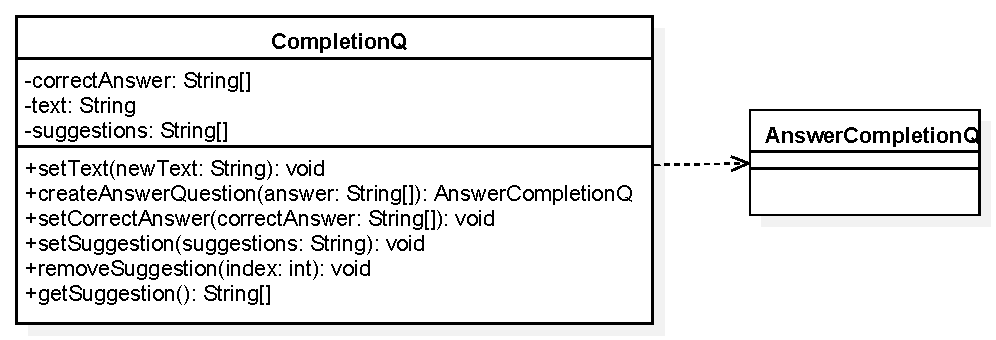
\includegraphics[width=\textwidth]{Img/quizzipedia-client-modelclient-services-questions-completionq.pdf}}
\caption[Schema Classe CompletionQ]{Schema Classe Quizzipedia::Client::ModelClient::Services::Questions::CompletionQ}
\end{figure}
\paragraph{Relazioni con altre classi}
\subparagraph{Uscenti}
\begin{itemize}
\item usa \cls{Quizzipedia::Client::ModelClient::Services::Questions::GenericQuestion} per aggiungi
\end{itemize}
\subsubsection{Classe \cls{GenericQuestion}}
Descrive le parti comuni a tutti i tipi di domanda presenti nel sistema.
\begin{figure}[H]
\centering
\noindent\makebox[\textwidth]{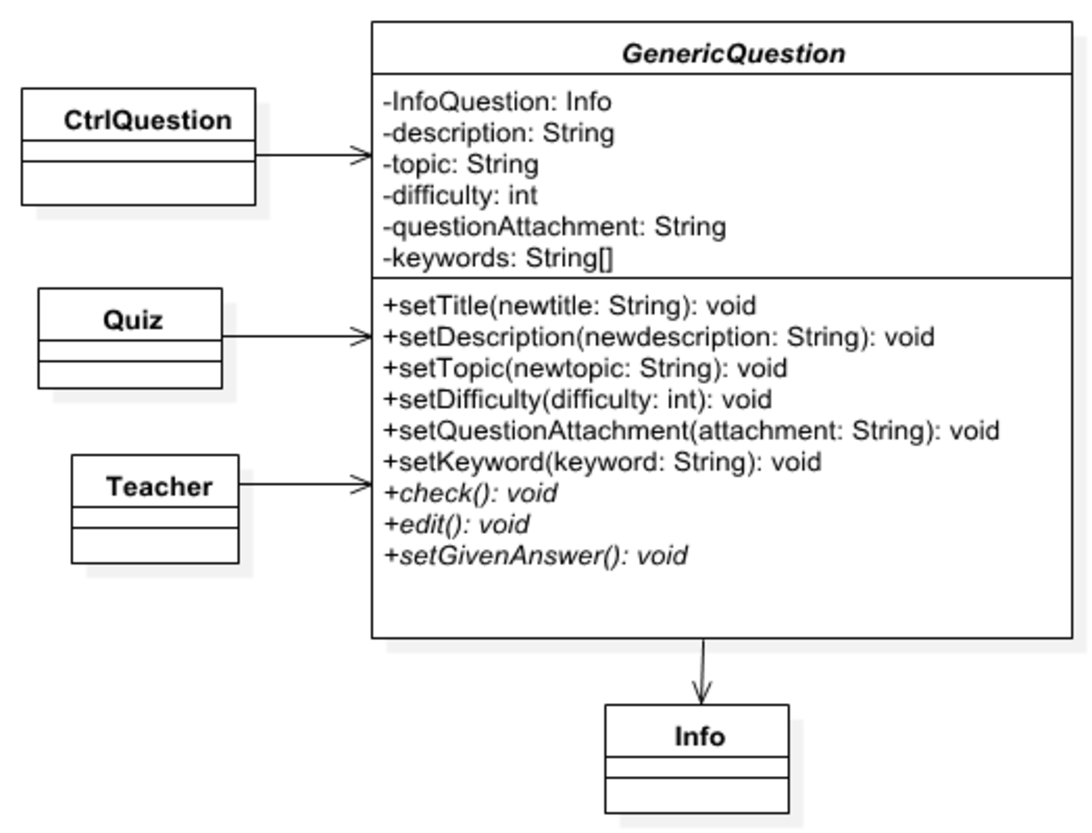
\includegraphics[width=\textwidth]{Img/quizzipedia-client-modelclient-services-questions-genericquestion.pdf}}
\caption[Schema Classe GenericQuestion]{Schema Classe Quizzipedia::Client::ModelClient::Services::Questions::GenericQuestion}
\end{figure}
\paragraph{Relazioni con altre classi}
\subparagraph{Entranti}
\begin{itemize}
\item usata da \cls{Quizzipedia::Client::ModelClient::Services::Answers::AnswerQuestion} per tenere traccia della domanda a cui corrisponde la risposta in questione
\item usata da \cls{Quizzipedia::Client::ModelClient::Services::Questions::CompletionQ} per aggiungi
\item usata da \cls{Quizzipedia::Client::ModelClient::Services::Questions::MatchingQ} per aggiungi
\item usata da \cls{Quizzipedia::Client::ModelClient::Services::Questions::MultipleChoiceQ} per aggiungi
\item usata da \cls{Quizzipedia::Client::ModelClient::Services::Questions::ShortAnswerQ} per aggiungi
\item usata da \cls{Quizzipedia::Client::ModelClient::Services::Questions::TrueFalseQ} per aggiungi
\item usata da \cls{Quizzipedia::Client::ModelClient::Services::Quiz} per aggiungi
\item usata da \cls{Quizzipedia::Client::ModelClient::Users::Teacher} per aggiungi
\item usata da \cls{Quizzipedia::Client::ViewModelClient::CtrlServices::CtrlQuestion} per aggiungi
\end{itemize}
\subsubsection{Classe \cls{MatchingQ}}
La struttura descrive le domande a collegamento. L'utente dovrà formare la risposta collegando le entrate da un numero variabile di colonne .
\begin{figure}[H]
\centering
\noindent\makebox[\textwidth]{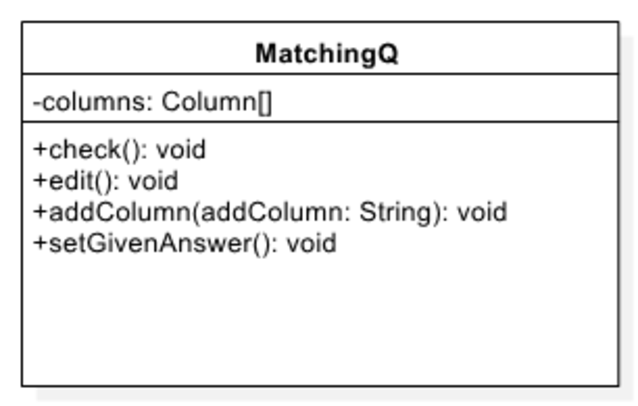
\includegraphics[width=\textwidth]{Img/quizzipedia-client-modelclient-services-questions-matchingq.pdf}}
\caption[Schema Classe MatchingQ]{Schema Classe Quizzipedia::Client::ModelClient::Services::Questions::MatchingQ}
\end{figure}
\paragraph{Relazioni con altre classi}
\subparagraph{Uscenti}
\begin{itemize}
\item usa \cls{Quizzipedia::Client::ModelClient::Services::Questions::Column} per aggiungi
\item usa \cls{Quizzipedia::Client::ModelClient::Services::Questions::GenericQuestion} per aggiungi
\end{itemize}
\subsubsection{Classe \cls{MultipleChoiceQ}}
La struttura descrive le domande a scelta multipla; viene presentata una lista di opzioni tra cui scegliere quelle corrette.
\begin{figure}[H]
\centering
\noindent\makebox[\textwidth]{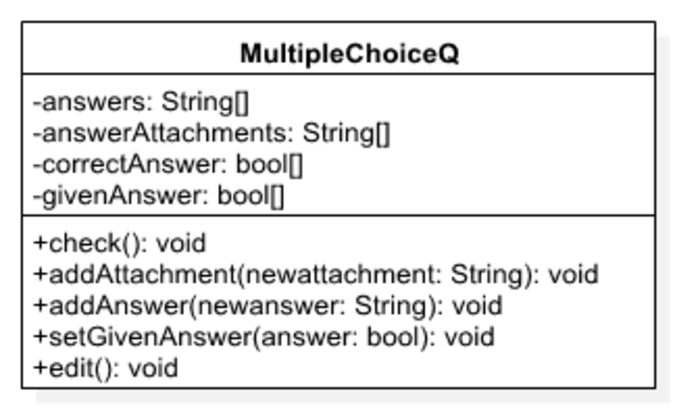
\includegraphics[width=\textwidth]{Img/quizzipedia-client-modelclient-services-questions-multiplechoiceq.pdf}}
\caption[Schema Classe MultipleChoiceQ]{Schema Classe Quizzipedia::Client::ModelClient::Services::Questions::MultipleChoiceQ}
\end{figure}
\paragraph{Relazioni con altre classi}
\subparagraph{Uscenti}
\begin{itemize}
\item usa \cls{Quizzipedia::Client::ModelClient::Services::Questions::GenericQuestion} per aggiungi
\end{itemize}
\subsubsection{Classe \cls{ShortAnswerQ}}
La struttura descrive le domande aperte, ovvero quelle la cui risposta consiste in un termine o una frase specifici.
\begin{figure}[H]
\centering
\noindent\makebox[\textwidth]{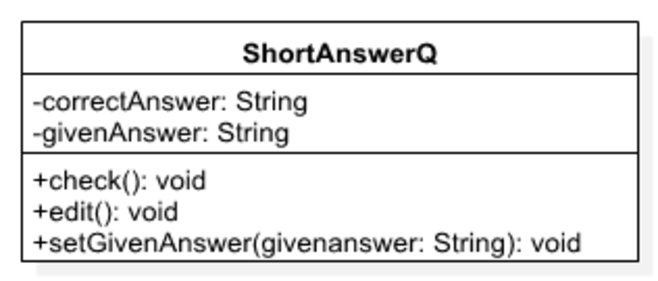
\includegraphics[width=\textwidth]{Img/quizzipedia-client-modelclient-services-questions-shortanswerq.pdf}}
\caption[Schema Classe ShortAnswerQ]{Schema Classe Quizzipedia::Client::ModelClient::Services::Questions::ShortAnswerQ}
\end{figure}
\paragraph{Relazioni con altre classi}
\subparagraph{Uscenti}
\begin{itemize}
\item usa \cls{Quizzipedia::Client::ModelClient::Services::Questions::GenericQuestion} per aggiungi
\end{itemize}
\subsubsection{Classe \cls{TrueFalseQ}}
Viene descritta la struttura delle domande che prevedono di decidere la veridicità di un'affermazione.
\begin{figure}[H]
\centering
\noindent\makebox[\textwidth]{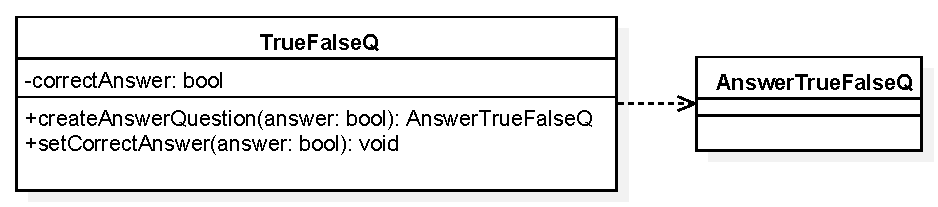
\includegraphics[width=\textwidth]{Img/quizzipedia-client-modelclient-services-questions-truefalseq.pdf}}
\caption[Schema Classe TrueFalseQ]{Schema Classe Quizzipedia::Client::ModelClient::Services::Questions::TrueFalseQ}
\end{figure}
\paragraph{Relazioni con altre classi}
\subparagraph{Uscenti}
\begin{itemize}
\item usa \cls{Quizzipedia::Client::ModelClient::Services::Questions::GenericQuestion} per aggiungi
\end{itemize}
\subsection{\pkg{Quizzipedia::Client::ModelClient::Statistics}}
Qui sono raccolte le classi con il compito di reperire informazioni sulle statistiche dal server e presentarle all'utente finale. Sono disponibili statistiche per le domande, per i quiz e per gli studenti di ogni classe.
\begin{figure}[H]
\centering
\noindent\makebox[\textwidth]{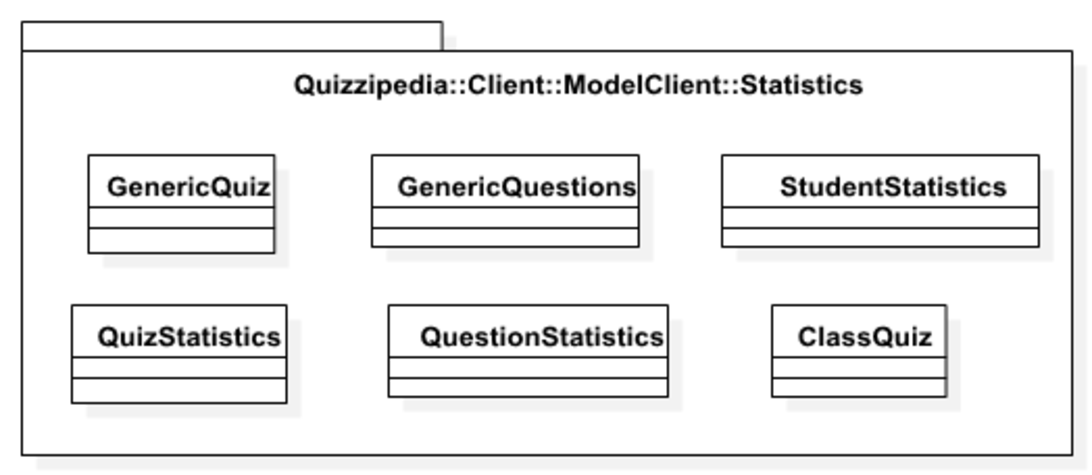
\includegraphics[width=\textwidth]{Img/quizzipedia-client-modelclient-statistics.pdf}}
\caption[Schema Componente Quizzipedia::Client::ModelClient::Statistics]{Schema Componente Quizzipedia::Client::ModelClient::Statistics}
\end{figure}
\subsubsection{Interazioni con altre componenti}
\begin{itemize}
\item \bold{Entranti}
\begin{itemize}
\item usata da \pkg{Quizzipedia::Client::ModelClient::Users} per aggiungi
\end{itemize}
\end{itemize}
\subsubsection{Classe \cls{QuestionStatistics}}
La classe raccoglie le statistiche principali riguardanti una singola domanda. Da qui è poi possibile risalire alla domanda.
\begin{figure}[H]
\centering
\noindent\makebox[\textwidth]{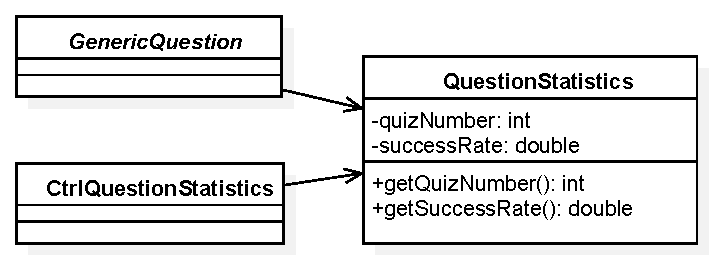
\includegraphics[width=\textwidth]{Img/quizzipedia-client-modelclient-statistics-questionstatistics.pdf}}
\caption[Schema Classe QuestionStatistics]{Schema Classe Quizzipedia::Client::ModelClient::Statistics::QuestionStatistics}
\end{figure}
\paragraph{Relazioni con altre classi}
\subparagraph{Entranti}
\begin{itemize}
\item usata da \cls{Quizzipedia::Server::ControllerServer::StatisticsManager::QuestionStatisticsFetcher} per 
\end{itemize}
\subsubsection{Classe \cls{QuizStatistics}}
La classe raccoglie le statistiche principali riguardanti un singolo quiz. Da qui è poi possibile ottenere il quiz in questione.
\begin{figure}[H]
\centering
\noindent\makebox[\textwidth]{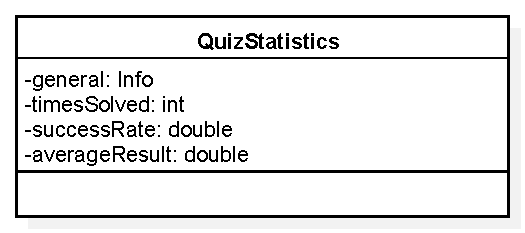
\includegraphics[width=\textwidth]{Img/quizzipedia-client-modelclient-statistics-quizstatistics.pdf}}
\caption[Schema Classe QuizStatistics]{Schema Classe Quizzipedia::Client::ModelClient::Statistics::QuizStatistics}
\end{figure}
\subsubsection{Classe \cls{StudentsStatisticsQuiz}}
Classe usata per visualizzare i studenti che hanno svolto un quiz specifico e il loro voto.
\begin{figure}[H]
\centering
\noindent\makebox[\textwidth]{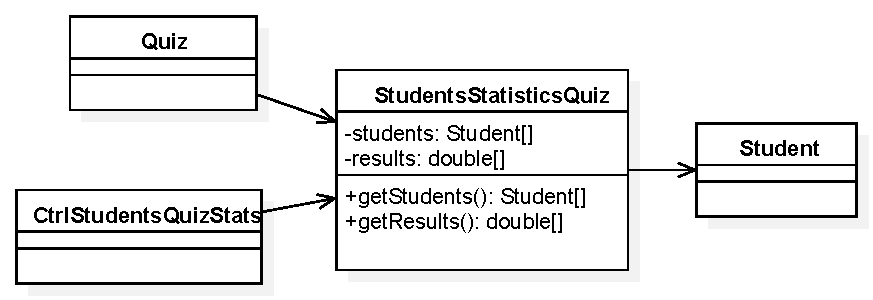
\includegraphics[width=\textwidth]{Img/quizzipedia-client-modelclient-statistics-studentsstatisticsquiz.pdf}}
\caption[Schema Classe StudentsStatisticsQuiz]{Schema Classe Quizzipedia::Client::ModelClient::Statistics::StudentsStatisticsQuiz}
\end{figure}
\subsection{\pkg{Quizzipedia::Client::ModelClient::Users}}
Raccoglie le classi necessarie a descrivere le diverse tipologie di utente che possono accedere al sistema.
\begin{figure}[H]
\centering
\noindent\makebox[\textwidth]{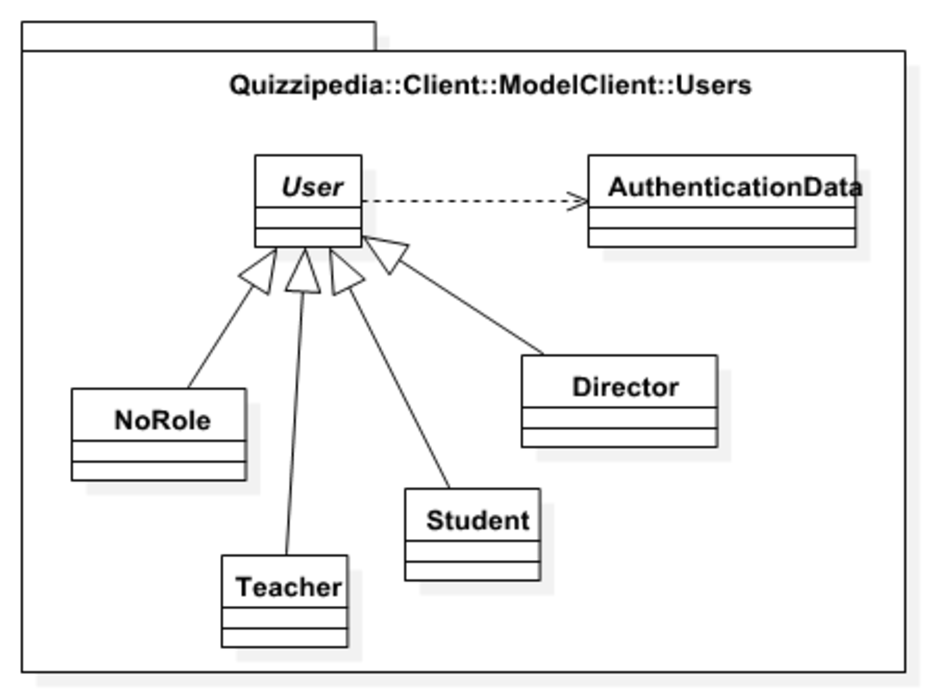
\includegraphics[width=\textwidth]{Img/quizzipedia-client-modelclient-users.pdf}}
\caption[Schema Componente Quizzipedia::Client::ModelClient::Users]{Schema Componente Quizzipedia::Client::ModelClient::Users}
\end{figure}
\subsubsection{Interazioni con altre componenti}
\begin{itemize}
\item \bold{Entranti}
\begin{itemize}
\item usata da \pkg{Quizzipedia::Client::ViewModelClient::CtrlUsers} per avere accesso alla struttura dei vari tipi di utente. In questo modo potrà compiere operazioni di modifica e manutenzione
\end{itemize}
\item \bold{Uscenti}
\begin{itemize}
\item usa \pkg{Quizzipedia::Client::ModelClient::Organizations} per organizzare gli utenti all'interno di enti e classi
\item usa \pkg{Quizzipedia::Client::ModelClient::Requests} per permettere agli utenti di effettuare richieste. Le richieste possono essere di ruolo o di classe
\item usa \pkg{Quizzipedia::Client::ModelClient::Services} per Permettere agli utenti di tenere traccia dello storico dei quiz svolti
\item usa \pkg{Quizzipedia::Client::ModelClient::Statistics} per aggiungi
\end{itemize}
\end{itemize}
\subsubsection{Classe \cls{AuthenticationData}}
Questa classe gestisce le informazioni di autenticazione comuni a tutti gli utenti.
\begin{figure}[H]
\centering
\noindent\makebox[\textwidth]{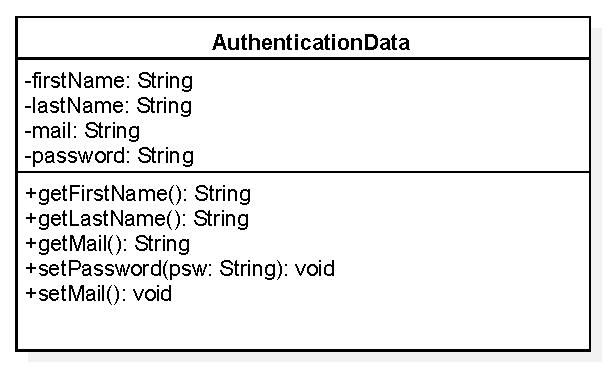
\includegraphics[width=\textwidth]{Img/quizzipedia-client-modelclient-users-authenticationdata.pdf}}
\caption[Schema Classe AuthenticationData]{Schema Classe Quizzipedia::Client::ModelClient::Users::AuthenticationData}
\end{figure}
\paragraph{Relazioni con altre classi}
\subparagraph{Entranti}
\begin{itemize}
\item usata da \cls{Quizzipedia::Client::ModelClient::Users::User} per aggiungi
\end{itemize}
\subsubsection{Classe \cls{Director}}
Rappresenta un responsabile, ovvero colui che gestisce docenti e studenti per ogni ente del sistema.
\begin{figure}[H]
\centering
\noindent\makebox[\textwidth]{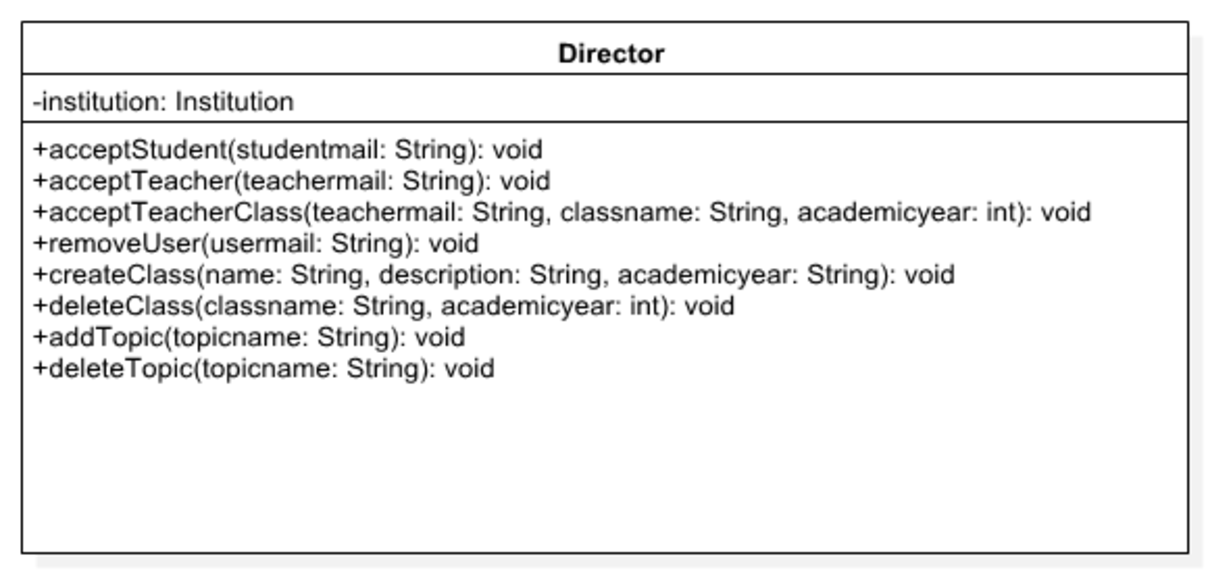
\includegraphics[width=\textwidth]{Img/quizzipedia-client-modelclient-users-director.pdf}}
\caption[Schema Classe Director]{Schema Classe Quizzipedia::Client::ModelClient::Users::Director}
\end{figure}
\paragraph{Relazioni con altre classi}
\subparagraph{Entranti}
\begin{itemize}
\item usata da \cls{Quizzipedia::Client::ViewModelClient::CtrlUsers::CtrlUserManager} per caricare un utente del tipo corretto
\end{itemize}
\subparagraph{Uscenti}
\begin{itemize}
\item usa \cls{Quizzipedia::Client::ModelClient::Services::Topics} per permettere al responsabile di modificare la lista dei possibili argomenti
\item usa \cls{Quizzipedia::Client::ModelClient::Users::User} per aggiungi
\end{itemize}
\subsubsection{Classe \cls{NoRole}}
Rappresenta gli utenti senza ruolo del sistema; coloro che si sono registrati e autenticati ma non hanno ancora fatto richiesta per l'assegnazione ad alcun ruolo.
\begin{figure}[H]
\centering
\noindent\makebox[\textwidth]{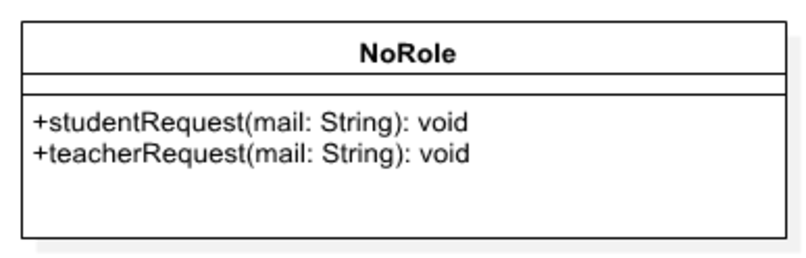
\includegraphics[width=\textwidth]{Img/quizzipedia-client-modelclient-users-norole.pdf}}
\caption[Schema Classe NoRole]{Schema Classe Quizzipedia::Client::ModelClient::Users::NoRole}
\end{figure}
\paragraph{Relazioni con altre classi}
\subparagraph{Entranti}
\begin{itemize}
\item usata da \cls{Quizzipedia::Client::ViewModelClient::CtrlUsers::CtrlUserManager} per caricare un utente del tipo corretto
\end{itemize}
\subparagraph{Uscenti}
\begin{itemize}
\item usa \cls{Quizzipedia::Client::ModelClient::Users::User} per aggiungi
\end{itemize}
\subsubsection{Classe \cls{Student}}
Rappresenta uno studente del sistema e implementa le sue funzioni specifiche oltre a quelle ereditate da utente.
\begin{figure}[H]
\centering
\noindent\makebox[\textwidth]{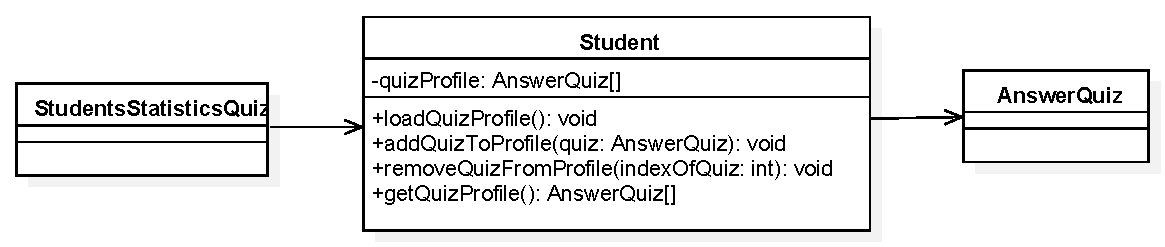
\includegraphics[width=\textwidth]{Img/quizzipedia-client-modelclient-users-student.pdf}}
\caption[Schema Classe Student]{Schema Classe Quizzipedia::Client::ModelClient::Users::Student}
\end{figure}
\paragraph{Relazioni con altre classi}
\subparagraph{Entranti}
\begin{itemize}
\item usata da \cls{Quizzipedia::Client::ViewModelClient::CtrlRequests::CtrlRequestClass} per 
\item usata da \cls{Quizzipedia::Client::ViewModelClient::CtrlUsers::CtrlUserManager} per caricare un utente del tipo corretto
\end{itemize}
\subparagraph{Uscenti}
\begin{itemize}
\item usa \cls{Quizzipedia::Client::ModelClient::Users::User} per aggiungi
\end{itemize}
\subsubsection{Classe \cls{Teacher}}
Rappresenta un docente del sistema e ne implementa le funzionalità specifiche in aggiunta a quelle comuni a tutti gli utenti.
\begin{figure}[H]
\centering
\noindent\makebox[\textwidth]{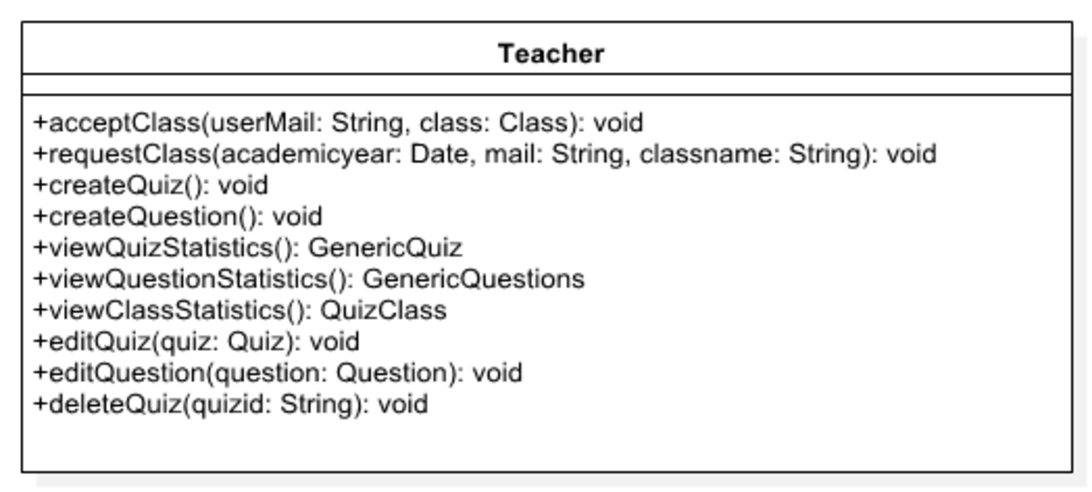
\includegraphics[width=\textwidth]{Img/quizzipedia-client-modelclient-users-teacher.pdf}}
\caption[Schema Classe Teacher]{Schema Classe Quizzipedia::Client::ModelClient::Users::Teacher}
\end{figure}
\paragraph{Relazioni con altre classi}
\subparagraph{Entranti}
\begin{itemize}
\item usata da \cls{Quizzipedia::Client::ViewModelClient::CtrlRequests::CtrlRequestClass} per 
\item usata da \cls{Quizzipedia::Client::ViewModelClient::CtrlUsers::CtrlUserManager} per caricare un utente del tipo corretto
\end{itemize}
\subparagraph{Uscenti}
\begin{itemize}
\item usa \cls{Quizzipedia::Client::ModelClient::Services::Questions::GenericQuestion} per aggiungi
\item usa \cls{Quizzipedia::Client::ModelClient::Services::Quiz} per aggiungi
\item usa \cls{Quizzipedia::Client::ModelClient::Users::User} per aggiungi
\end{itemize}
\subsubsection{Classe \cls{User}}
Questa è una classe astratta e raccoglie le funzionalità comuni a tutti gli utenti.
\begin{figure}[H]
\centering
\noindent\makebox[\textwidth]{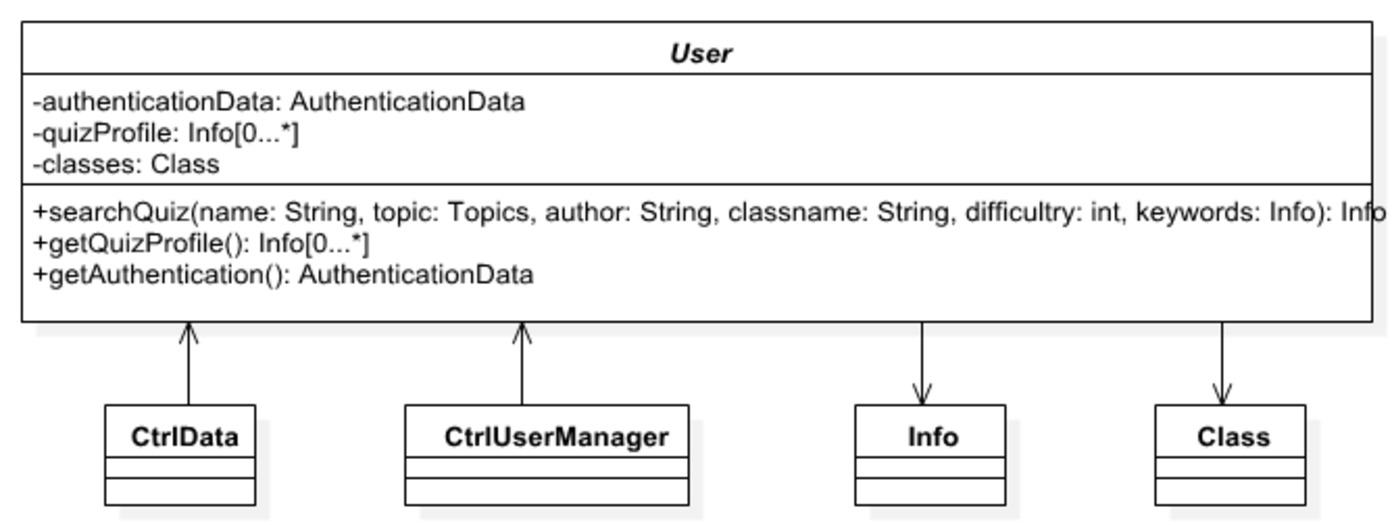
\includegraphics[width=\textwidth]{Img/quizzipedia-client-modelclient-users-user.pdf}}
\caption[Schema Classe User]{Schema Classe Quizzipedia::Client::ModelClient::Users::User}
\end{figure}
\paragraph{Relazioni con altre classi}
\subparagraph{Entranti}
\begin{itemize}
\item usata da \cls{Quizzipedia::Client::ModelClient::Services::Answers::AnswerQuestion} per tenere traccia di quale utente ha dato la risposta in questione
\item usata da \cls{Quizzipedia::Client::ModelClient::Users::Director} per aggiungi
\item usata da \cls{Quizzipedia::Client::ModelClient::Users::NoRole} per aggiungi
\item usata da \cls{Quizzipedia::Client::ModelClient::Users::Student} per aggiungi
\item usata da \cls{Quizzipedia::Client::ModelClient::Users::Teacher} per aggiungi
\end{itemize}
\subparagraph{Uscenti}
\begin{itemize}
\item usa \cls{Quizzipedia::Client::ModelClient::Organizations::Class} per tenere traccia delle classi dell'ente
a cui l'utente è iscritto, o come docente, o come studente
\item usa \cls{Quizzipedia::Client::ModelClient::Users::AuthenticationData} per aggiungi
\end{itemize}
\subsection{\pkg{Quizzipedia::Client::ViewClient}}
Racchiude tutte le componenti necessarie per presentare il prodotto all'utente.
Grazie all'uso di Angular.js ogni modifica svolta dall'utente si ripercuoterà automaticamente a sulla componente model, attraverso il controller, per mantenere sempre le informazioni consistenti e aggiornate.
Con l'uso invece di Bootstrap e Fabric.js a livello di grafica web risulta semplificata l'impaginazione delle singole pagine web dedicate all'utente e alla gestione di allegati non testuali all'interno di domande.
\begin{figure}[H]
\centering
\noindent\makebox[\textwidth]{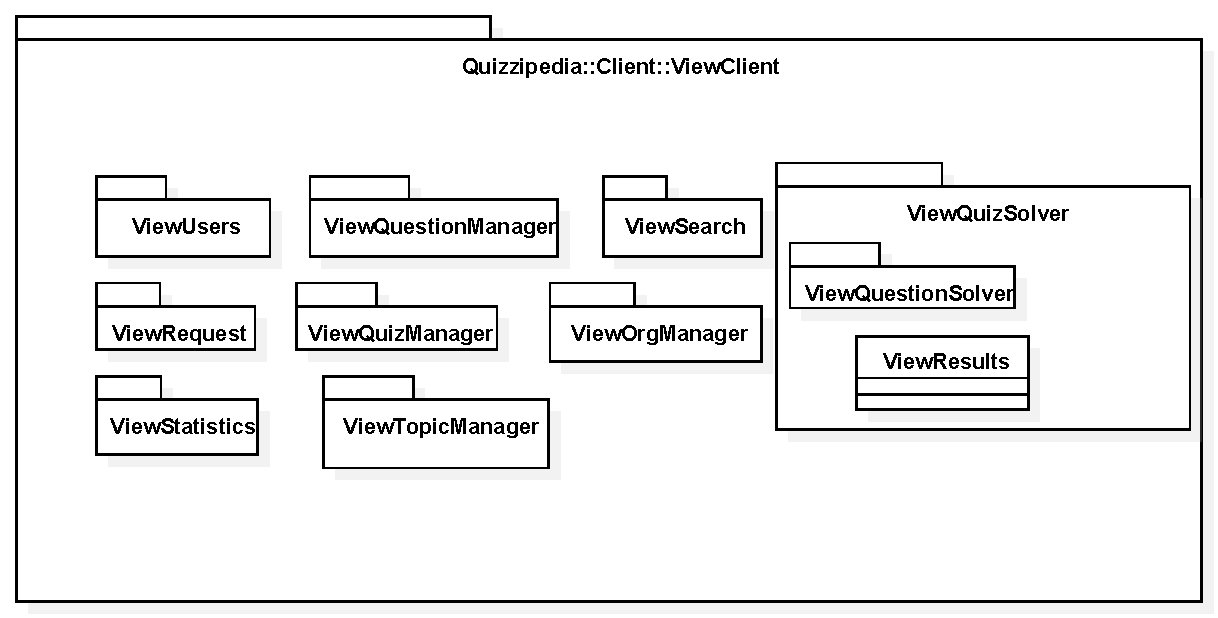
\includegraphics[width=\textwidth]{Img/quizzipedia-client-viewclient.pdf}}
\caption[Schema Componente Quizzipedia::Client::ViewClient]{Schema Componente Quizzipedia::Client::ViewClient}
\end{figure}
\subsubsection{Componenti contenute}
\begin{itemize}
\item \pkg{Quizzipedia::Client::ViewClient::ViewOrgManager}
\item \pkg{Quizzipedia::Client::ViewClient::ViewQuestionManager}
\item \pkg{Quizzipedia::Client::ViewClient::ViewQuizManager}
\item \pkg{Quizzipedia::Client::ViewClient::ViewQuizSolver}
\item \pkg{Quizzipedia::Client::ViewClient::ViewRequests}
\item \pkg{Quizzipedia::Client::ViewClient::ViewSearch}
\item \pkg{Quizzipedia::Client::ViewClient::ViewStatistics}
\item \pkg{Quizzipedia::Client::ViewClient::ViewTopicManager}
\item \pkg{Quizzipedia::Client::ViewClient::ViewUsers}
\end{itemize}
\subsubsection{Interazioni con altre componenti}
\begin{itemize}
\item \bold{Uscenti}
\begin{itemize}
\item usa \pkg{Quizzipedia::Client::ViewModelClient} per aggiungi
\end{itemize}
\end{itemize}
\subsection{\pkg{Quizzipedia::Client::ViewClient::ViewOrgManager}}
Qui sono raccolte le classi responsabili della presentazione delle pagine da cui sarà possibile gestire le classi e gli enti presenti in Quizzipedia.
\begin{figure}[H]
\centering
\noindent\makebox[\textwidth]{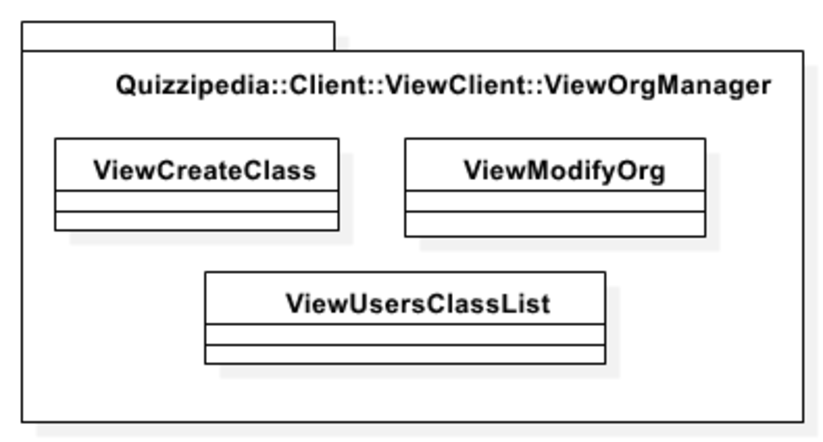
\includegraphics[width=\textwidth]{Img/quizzipedia-client-viewclient-vieworgmanager.pdf}}
\caption[Schema Componente Quizzipedia::Client::ViewClient::ViewOrgManager]{Schema Componente Quizzipedia::Client::ViewClient::ViewOrgManager}
\end{figure}
\subsubsection{Interazioni con altre componenti}
\begin{itemize}
\item \bold{Uscenti}
\begin{itemize}
\item usa \pkg{Quizzipedia::Client::ViewModelClient::CtrlOrganization} per aggiungi
\end{itemize}
\end{itemize}
\subsubsection{Classe \cls{ViewCreateClass}}
Classe responsabile della creazione della pagina da cui sarà possibile creare una nuova classe.
\begin{figure}[H]
\centering
\noindent\makebox[\textwidth]{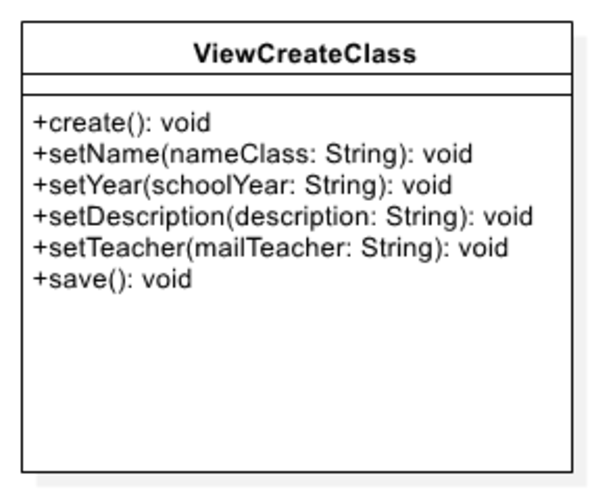
\includegraphics[width=\textwidth]{Img/quizzipedia-client-viewclient-vieworgmanager-viewcreateclass.pdf}}
\caption[Schema Classe ViewCreateClass]{Schema Classe Quizzipedia::Client::ViewClient::ViewOrgManager::ViewCreateClass}
\end{figure}
\subsubsection{Classe \cls{ViewModifyOrg}}
Presenta all'utente la pagina da cui sarà possibile modificare le informazioni su una classe o su un ente esistente.
\begin{figure}[H]
\centering
\noindent\makebox[\textwidth]{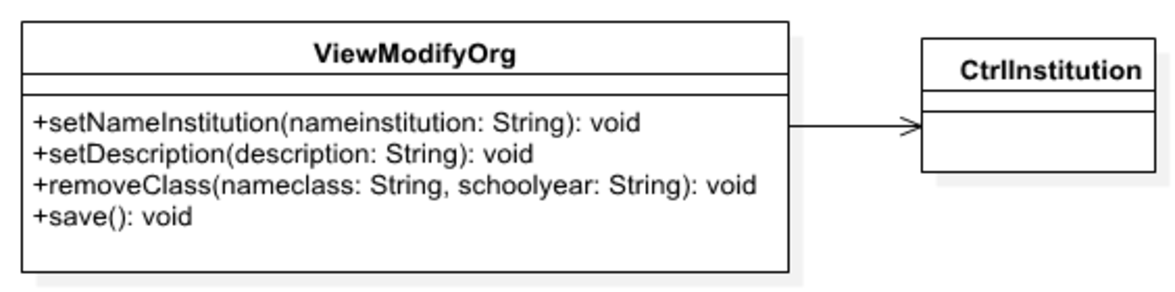
\includegraphics[width=\textwidth]{Img/quizzipedia-client-viewclient-vieworgmanager-viewmodifyorg.pdf}}
\caption[Schema Classe ViewModifyOrg]{Schema Classe Quizzipedia::Client::ViewClient::ViewOrgManager::ViewModifyOrg}
\end{figure}
\paragraph{Relazioni con altre classi}
\subparagraph{Uscenti}
\begin{itemize}
\item usa \cls{Quizzipedia::Client::ViewModelClient::CtrlOrganization::CtrlInstitution} per passare al controller i dati immessi dall'utente durante le operazioni di modifica, creazione o rimozione di una classe di un istituto
\end{itemize}
\subsubsection{Classe \cls{ViewUsersClassList}}
La classe si occupa di presentare una lista degli utenti iscritti alla classe e altre informazioni aggiuntive.
\begin{figure}[H]
\centering
\noindent\makebox[\textwidth]{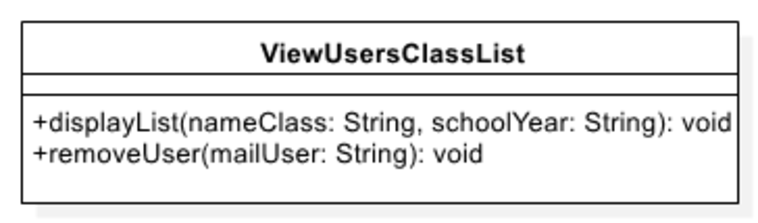
\includegraphics[width=\textwidth]{Img/quizzipedia-client-viewclient-vieworgmanager-viewusersclasslist.pdf}}
\caption[Schema Classe ViewUsersClassList]{Schema Classe Quizzipedia::Client::ViewClient::ViewOrgManager::ViewUsersClassList}
\end{figure}
\subsection{\pkg{Quizzipedia::Client::ViewClient::ViewQuestionManager}}
Qui sono raccolte le classi responsabili della presentazione delle pagine da cui sarà possibile gestire le domande.
\begin{figure}[H]
\centering
\noindent\makebox[\textwidth]{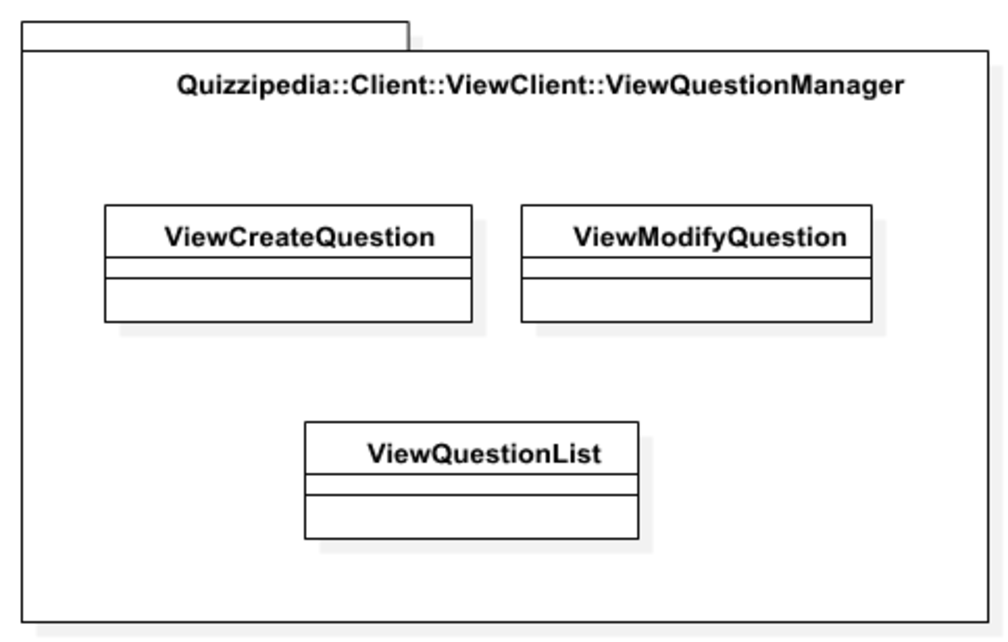
\includegraphics[width=\textwidth]{Img/quizzipedia-client-viewclient-viewquestionmanager.pdf}}
\caption[Schema Componente Quizzipedia::Client::ViewClient::ViewQuestionManager]{Schema Componente Quizzipedia::Client::ViewClient::ViewQuestionManager}
\end{figure}
\subsubsection{Interazioni con altre componenti}
\begin{itemize}
\item \bold{Uscenti}
\begin{itemize}
\item usa \pkg{Quizzipedia::Client::ViewModelClient::CtrlServices} per aggiungi
\end{itemize}
\end{itemize}
\subsubsection{Classe \cls{ViewCreateQuestion}}
Presenta la pagina da cui sarà possibile creare una nuova domanda.
\begin{figure}[H]
\centering
\noindent\makebox[\textwidth]{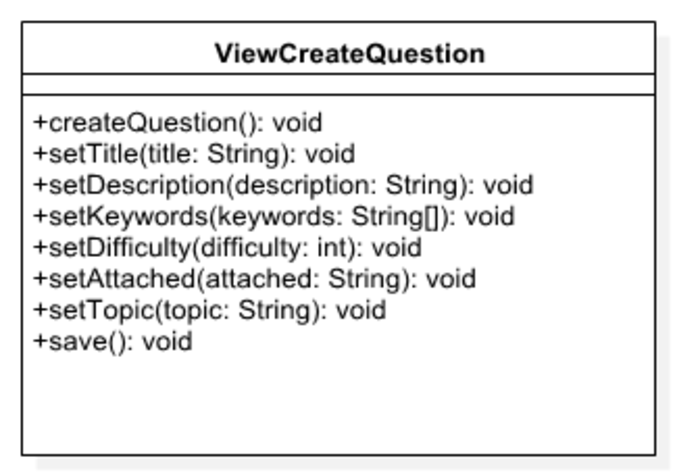
\includegraphics[width=\textwidth]{Img/quizzipedia-client-viewclient-viewquestionmanager-viewcreatequestion.pdf}}
\caption[Schema Classe ViewCreateQuestion]{Schema Classe Quizzipedia::Client::ViewClient::ViewQuestionManager::ViewCreateQuestion}
\end{figure}
\paragraph{Relazioni con altre classi}
\subparagraph{Uscenti}
\begin{itemize}
\item usa \cls{Quizzipedia::Client::ViewModelClient::CtrlServices::CtrlQuestion} per aggiungi
\end{itemize}
\subsubsection{Classe \cls{ViewModifyQuestion}}
Gestisce la visualizzazione della pagina da cui è possibile modificare una domanda esistente.
\begin{figure}[H]
\centering
\noindent\makebox[\textwidth]{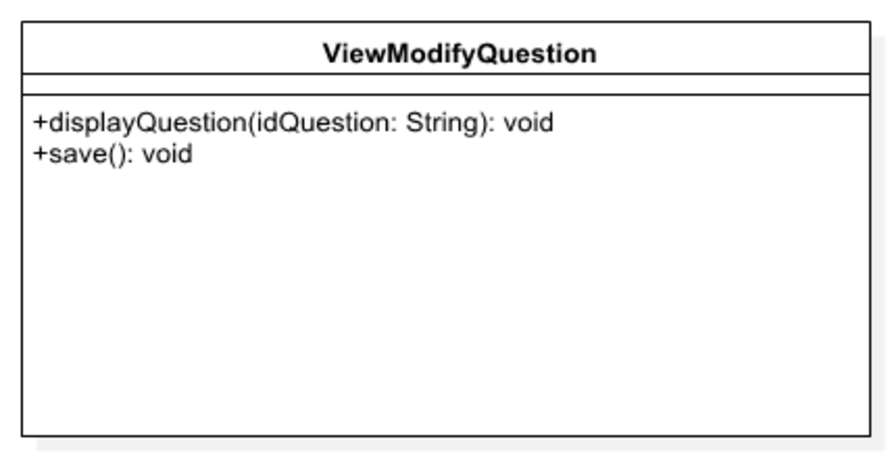
\includegraphics[width=\textwidth]{Img/quizzipedia-client-viewclient-viewquestionmanager-viewmodifyquestion.pdf}}
\caption[Schema Classe ViewModifyQuestion]{Schema Classe Quizzipedia::Client::ViewClient::ViewQuestionManager::ViewModifyQuestion}
\end{figure}
\paragraph{Relazioni con altre classi}
\subparagraph{Uscenti}
\begin{itemize}
\item usa \cls{Quizzipedia::Client::ViewModelClient::CtrlServices::CtrlQuestion} per aggiungi
\end{itemize}
\subsubsection{Classe \cls{ViewQuestionList}}
Presenta all'utente il pannello da cui sarà possibile visualizzare una lista di informazioni riassuntive sulle domande e compiere alcune operazioni su di esse.
\begin{figure}[H]
\centering
\noindent\makebox[\textwidth]{\includegraphics[width=\textwidth]{Img/quizzipedia-client-viewclient-viewquestionmanager-viewquestionlist.pdf}}
\caption[Schema Classe ViewQuestionList]{Schema Classe Quizzipedia::Client::ViewClient::ViewQuestionManager::ViewQuestionList}
\end{figure}
\paragraph{Relazioni con altre classi}
\subparagraph{Uscenti}
\begin{itemize}
\item usa \cls{Quizzipedia::Client::ViewModelClient::CtrlServices::CtrlQuestion} per aggiungi
\end{itemize}
\subsection{\pkg{Quizzipedia::Client::ViewClient::ViewQuizManager}}
Qui sono raccolte le classi responsabili della presentazione delle pagine da cui sarà possibile gestire i quiz.
\begin{figure}[H]
\centering
\noindent\makebox[\textwidth]{\includegraphics[width=\textwidth]{Img/quizzipedia-client-viewclient-viewquizmanager.pdf}}
\caption[Schema Componente Quizzipedia::Client::ViewClient::ViewQuizManager]{Schema Componente Quizzipedia::Client::ViewClient::ViewQuizManager}
\end{figure}
\subsubsection{Interazioni con altre componenti}
\begin{itemize}
\item \bold{Uscenti}
\begin{itemize}
\item usa \pkg{Quizzipedia::Client::ViewModelClient::CtrlServices} per aggiungi
\end{itemize}
\end{itemize}
\subsubsection{Classe \cls{ViewCreateQuiz}}
Presenta la pagina da cui sarà possibile creare un nuovo quiz.
\begin{figure}[H]
\centering
\noindent\makebox[\textwidth]{\includegraphics[width=\textwidth]{Img/quizzipedia-client-viewclient-viewquizmanager-viewcreatequiz.pdf}}
\caption[Schema Classe ViewCreateQuiz]{Schema Classe Quizzipedia::Client::ViewClient::ViewQuizManager::ViewCreateQuiz}
\end{figure}
\paragraph{Relazioni con altre classi}
\subparagraph{Uscenti}
\begin{itemize}
\item usa \cls{Quizzipedia::Client::ViewModelClient::CtrlServices::CtrlQuiz} per aggiungi
\end{itemize}
\subsubsection{Classe \cls{ViewModifyQuiz}}
Presenta all'utente una pagina da cui è possibile modificare un quiz esistente.
\begin{figure}[H]
\centering
\noindent\makebox[\textwidth]{\includegraphics[width=\textwidth]{Img/quizzipedia-client-viewclient-viewquizmanager-viewmodifyquiz.pdf}}
\caption[Schema Classe ViewModifyQuiz]{Schema Classe Quizzipedia::Client::ViewClient::ViewQuizManager::ViewModifyQuiz}
\end{figure}
\paragraph{Relazioni con altre classi}
\subparagraph{Uscenti}
\begin{itemize}
\item usa \cls{Quizzipedia::Client::ViewModelClient::CtrlServices::CtrlQuiz} per aggiungi
\end{itemize}
\subsubsection{Classe \cls{ViewQuizList}}
Carica una pagina contenente una lista con informazioni riassuntive sui quiz e un pannello da cui sarà possibile svolgere delle operazioni sugli stessi.
\begin{figure}[H]
\centering
\noindent\makebox[\textwidth]{\includegraphics[width=\textwidth]{Img/quizzipedia-client-viewclient-viewquizmanager-viewquizlist.pdf}}
\caption[Schema Classe ViewQuizList]{Schema Classe Quizzipedia::Client::ViewClient::ViewQuizManager::ViewQuizList}
\end{figure}
\paragraph{Relazioni con altre classi}
\subparagraph{Uscenti}
\begin{itemize}
\item usa \cls{Quizzipedia::Client::ViewModelClient::CtrlServices::CtrlQuiz} per aggiungi
\end{itemize}
\subsection{\pkg{Quizzipedia::Client::ViewClient::ViewQuizSolver}}
Il componente raccoglie le classi necessarie alla visualizzazione delle pagine da cui sarà possibile svolgere quiz.
\begin{figure}[H]
\centering
\noindent\makebox[\textwidth]{\includegraphics[width=\textwidth]{Img/quizzipedia-client-viewclient-viewquizsolver.pdf}}
\caption[Schema Componente Quizzipedia::Client::ViewClient::ViewQuizSolver]{Schema Componente Quizzipedia::Client::ViewClient::ViewQuizSolver}
\end{figure}
\subsubsection{Componenti contenute}
\begin{itemize}
\item \pkg{Quizzipedia::Client::ViewClient::ViewQuizSolver::ViewQuestionSolver}
\end{itemize}
\subsubsection{Interazioni con altre componenti}
\begin{itemize}
\item \bold{Uscenti}
\begin{itemize}
\item usa \pkg{Quizzipedia::Client::ViewModelClient::CtrlServices} per aggiungi
\end{itemize}
\end{itemize}
\subsubsection{Classe \cls{ViewResults}}
La classe ha il compito di costruire la pagina da cui sarà possibile vedere l'esito di un quiz.
\begin{figure}[H]
\centering
\noindent\makebox[\textwidth]{\includegraphics[width=\textwidth]{Img/quizzipedia-client-viewclient-viewquizsolver-viewresults.pdf}}
\caption[Schema Classe ViewResults]{Schema Classe Quizzipedia::Client::ViewClient::ViewQuizSolver::ViewResults}
\end{figure}
\paragraph{Relazioni con altre classi}
\subparagraph{Uscenti}
\begin{itemize}
\item usa \cls{Quizzipedia::Client::ViewModelClient::CtrlServices::CtrlQuiz} per aggiungi
\end{itemize}
\subsection{\pkg{Quizzipedia::Client::ViewClient::ViewQuizSolver::ViewQuestionSolver}}
Il componente raccoglie le classi necessarie alla visualizzazione delle pagine da cui sarà possibile rispondere alle singole domande.
\begin{figure}[H]
\centering
\noindent\makebox[\textwidth]{\includegraphics[width=\textwidth]{Img/quizzipedia-client-viewclient-viewquizsolver-viewquestionsolver.pdf}}
\caption[Schema Componente Quizzipedia::Client::ViewClient::ViewQuizSolver::ViewQuestionSolver]{Schema Componente Quizzipedia::Client::ViewClient::ViewQuizSolver::ViewQuestionSolver}
\end{figure}
\subsubsection{Interazioni con altre componenti}
\begin{itemize}
\item \bold{Uscenti}
\begin{itemize}
\item usa \pkg{Quizzipedia::Client::ViewModelClient::CtrlServices} per 
\end{itemize}
\end{itemize}
\subsubsection{Classe \cls{ViewCompletionQ}}
Presenta all'utente la pagina da cui sarà possibile rispondere a una domanda a completamento.
\begin{figure}[H]
\centering
\noindent\makebox[\textwidth]{\includegraphics[width=\textwidth]{Img/quizzipedia-client-viewclient-viewquizsolver-viewquestionsolver-viewcompletionq.pdf}}
\caption[Schema Classe ViewCompletionQ]{Schema Classe Quizzipedia::Client::ViewClient::ViewQuizSolver::ViewQuestionSolver::ViewCompletionQ}
\end{figure}
\paragraph{Relazioni con altre classi}
\subparagraph{Uscenti}
\begin{itemize}
\item usa \cls{Quizzipedia::Client::ViewModelClient::CtrlServices::CtrlQuestion} per aggiungi
\end{itemize}
\subsubsection{Classe \cls{ViewMatchingQ}}
Presenta all'utente la pagina da cui sarà possibile rispondere a una domanda a collegamenti.
\begin{figure}[H]
\centering
\noindent\makebox[\textwidth]{\includegraphics[width=\textwidth]{Img/quizzipedia-client-viewclient-viewquizsolver-viewquestionsolver-viewmatchingq.pdf}}
\caption[Schema Classe ViewMatchingQ]{Schema Classe Quizzipedia::Client::ViewClient::ViewQuizSolver::ViewQuestionSolver::ViewMatchingQ}
\end{figure}
\paragraph{Relazioni con altre classi}
\subparagraph{Uscenti}
\begin{itemize}
\item usa \cls{Quizzipedia::Client::ViewModelClient::CtrlServices::CtrlQuestion} per aggiungi
\end{itemize}
\subsubsection{Classe \cls{ViewMultipleChoiceQ}}
Presenta all'utente la pagina da cui sarà possibile rispondere a una domanda a risposta multipla.
\begin{figure}[H]
\centering
\noindent\makebox[\textwidth]{\includegraphics[width=\textwidth]{Img/quizzipedia-client-viewclient-viewquizsolver-viewquestionsolver-viewmultiplechoiceq.pdf}}
\caption[Schema Classe ViewMultipleChoiceQ]{Schema Classe Quizzipedia::Client::ViewClient::ViewQuizSolver::ViewQuestionSolver::ViewMultipleChoiceQ}
\end{figure}
\paragraph{Relazioni con altre classi}
\subparagraph{Uscenti}
\begin{itemize}
\item usa \cls{Quizzipedia::Client::ViewModelClient::CtrlServices::CtrlQuestion} per aggiungi
\end{itemize}
\subsubsection{Classe \cls{ViewShortAnswerQ}}
Presenta all'utente la pagina da cui sarà possibile rispondere a una domanda a risposta aperta.
\begin{figure}[H]
\centering
\noindent\makebox[\textwidth]{\includegraphics[width=\textwidth]{Img/quizzipedia-client-viewclient-viewquizsolver-viewquestionsolver-viewshortanswerq.pdf}}
\caption[Schema Classe ViewShortAnswerQ]{Schema Classe Quizzipedia::Client::ViewClient::ViewQuizSolver::ViewQuestionSolver::ViewShortAnswerQ}
\end{figure}
\paragraph{Relazioni con altre classi}
\subparagraph{Uscenti}
\begin{itemize}
\item usa \cls{Quizzipedia::Client::ViewModelClient::CtrlServices::CtrlQuestion} per aggiungi
\end{itemize}
\subsubsection{Classe \cls{ViewTrueFalseQ}}
Presenta all'utente la pagina da cui sarà possibile rispondere a una domanda di tipo vero/falso.
\begin{figure}[H]
\centering
\noindent\makebox[\textwidth]{\includegraphics[width=\textwidth]{Img/quizzipedia-client-viewclient-viewquizsolver-viewquestionsolver-viewtruefalseq.pdf}}
\caption[Schema Classe ViewTrueFalseQ]{Schema Classe Quizzipedia::Client::ViewClient::ViewQuizSolver::ViewQuestionSolver::ViewTrueFalseQ}
\end{figure}
\paragraph{Relazioni con altre classi}
\subparagraph{Uscenti}
\begin{itemize}
\item usa \cls{Quizzipedia::Client::ViewModelClient::CtrlServices::CtrlQuestion} per aggiungi
\end{itemize}
\subsection{\pkg{Quizzipedia::Client::ViewClient::ViewRequests}}
Qui sono raccolte le pagine che permettono all'utente di gestire le richieste di ruolo e classe.
\begin{figure}[H]
\centering
\noindent\makebox[\textwidth]{\includegraphics[width=\textwidth]{Img/quizzipedia-client-viewclient-viewrequests.pdf}}
\caption[Schema Componente Quizzipedia::Client::ViewClient::ViewRequests]{Schema Componente Quizzipedia::Client::ViewClient::ViewRequests}
\end{figure}
\subsubsection{Interazioni con altre componenti}
\begin{itemize}
\item \bold{Uscenti}
\begin{itemize}
\item usa \pkg{Quizzipedia::Client::ViewModelClient::CtrlRequests} per aggiungi
\end{itemize}
\end{itemize}
\subsubsection{Classe \cls{RequestRole}}
Costruisce la pagina da cui l'utente potrà richiedere un ruolo (studente o docente).
\begin{figure}[H]
\centering
\noindent\makebox[\textwidth]{\includegraphics[width=\textwidth]{Img/quizzipedia-client-viewclient-viewrequests-requestrole.pdf}}
\caption[Schema Classe RequestRole]{Schema Classe Quizzipedia::Client::ViewClient::ViewRequests::RequestRole}
\end{figure}
\paragraph{Relazioni con altre classi}
\subparagraph{Uscenti}
\begin{itemize}
\item usa \cls{Quizzipedia::Client::ViewModelClient::CtrlRequests::CtrlRequestRole} per aggiungi
\end{itemize}
\subsubsection{Classe \cls{SendRequests}}
Costruisce la pagina da cui l'utente potrà richiedere di entrare in una classe.
\begin{figure}[H]
\centering
\noindent\makebox[\textwidth]{\includegraphics[width=\textwidth]{Img/quizzipedia-client-viewclient-viewrequests-sendrequests.pdf}}
\caption[Schema Classe SendRequests]{Schema Classe Quizzipedia::Client::ViewClient::ViewRequests::SendRequests}
\end{figure}
\paragraph{Relazioni con altre classi}
\subparagraph{Uscenti}
\begin{itemize}
\item usa \cls{Quizzipedia::Client::ViewModelClient::CtrlRequests::CtrlRequestClass} per aggiungi
\end{itemize}
\subsubsection{Classe \cls{ViewClassList}}
Classe responsabile della visualizzazione del pannello da cui sarà possibile gestire le richieste di inserimento in una classe.
\begin{figure}[H]
\centering
\noindent\makebox[\textwidth]{\includegraphics[width=\textwidth]{Img/quizzipedia-client-viewclient-viewrequests-viewclasslist.pdf}}
\caption[Schema Classe ViewClassList]{Schema Classe Quizzipedia::Client::ViewClient::ViewRequests::ViewClassList}
\end{figure}
\paragraph{Relazioni con altre classi}
\subparagraph{Uscenti}
\begin{itemize}
\item usa \cls{Quizzipedia::Client::ViewModelClient::CtrlRequests::CtrlRequestClass} per aggiungi
\end{itemize}
\subsubsection{Classe \cls{ViewRolesList}}
Classe responsabile della visualizzazione del pannello da cui sarà possibile gestire le richieste di assegnazione di ruolo.
\begin{figure}[H]
\centering
\noindent\makebox[\textwidth]{\includegraphics[width=\textwidth]{Img/quizzipedia-client-viewclient-viewrequests-viewroleslist.pdf}}
\caption[Schema Classe ViewRolesList]{Schema Classe Quizzipedia::Client::ViewClient::ViewRequests::ViewRolesList}
\end{figure}
\paragraph{Relazioni con altre classi}
\subparagraph{Uscenti}
\begin{itemize}
\item usa \cls{Quizzipedia::Client::ViewModelClient::CtrlRequests::CtrlRequestRole} per aggiungi
\end{itemize}
\subsection{\pkg{Quizzipedia::Client::ViewClient::ViewSearch}}
Il componente contiene le classi responsabili della creazione delle pagine da cui sarà possibile ricercare domande, quiz e classi.
\begin{figure}[H]
\centering
\noindent\makebox[\textwidth]{\includegraphics[width=\textwidth]{Img/quizzipedia-client-viewclient-viewsearch.pdf}}
\caption[Schema Componente Quizzipedia::Client::ViewClient::ViewSearch]{Schema Componente Quizzipedia::Client::ViewClient::ViewSearch}
\end{figure}
\subsubsection{Interazioni con altre componenti}
\begin{itemize}
\item \bold{Uscenti}
\begin{itemize}
\item usa \pkg{Quizzipedia::Client::ViewModelClient::CtrlOrganization} per aggiungi
\item usa \pkg{Quizzipedia::Client::ViewModelClient::CtrlServices} per aggiungi
\end{itemize}
\end{itemize}
\subsubsection{Classe \cls{ViewSearchClass}}
La classe carica la pagina da cui sarà possibile ricercare classi all'interno di un ente.
\begin{figure}[H]
\centering
\noindent\makebox[\textwidth]{\includegraphics[width=\textwidth]{Img/quizzipedia-client-viewclient-viewsearch-viewsearchclass.pdf}}
\caption[Schema Classe ViewSearchClass]{Schema Classe Quizzipedia::Client::ViewClient::ViewSearch::ViewSearchClass}
\end{figure}
\paragraph{Relazioni con altre classi}
\subparagraph{Uscenti}
\begin{itemize}
\item usa \cls{Quizzipedia::Client::ViewModelClient::CtrlOrganization::CtrlInstitution} per 
\end{itemize}
\subsubsection{Classe \cls{ViewSearchQuestion}}
Classe che ha il compito di caricare la pagina da cui sarà possibile effettuare la ricerca di domande.
\begin{figure}[H]
\centering
\noindent\makebox[\textwidth]{\includegraphics[width=\textwidth]{Img/quizzipedia-client-viewclient-viewsearch-viewsearchquestion.pdf}}
\caption[Schema Classe ViewSearchQuestion]{Schema Classe Quizzipedia::Client::ViewClient::ViewSearch::ViewSearchQuestion}
\end{figure}
\paragraph{Relazioni con altre classi}
\subparagraph{Uscenti}
\begin{itemize}
\item usa \cls{Quizzipedia::Client::ViewModelClient::CtrlServices::CtrlSearch} per aggiungi
\end{itemize}
\subsubsection{Classe \cls{ViewSearchQuiz}}
Raccoglie i metodi necessari alla creazione della pagina da cui sarà possibile cercare un quiz.
\begin{figure}[H]
\centering
\noindent\makebox[\textwidth]{\includegraphics[width=\textwidth]{Img/quizzipedia-client-viewclient-viewsearch-viewsearchquiz.pdf}}
\caption[Schema Classe ViewSearchQuiz]{Schema Classe Quizzipedia::Client::ViewClient::ViewSearch::ViewSearchQuiz}
\end{figure}
\paragraph{Relazioni con altre classi}
\subparagraph{Uscenti}
\begin{itemize}
\item usa \cls{Quizzipedia::Client::ViewModelClient::CtrlServices::CtrlSearch} per aggiungi
\end{itemize}
\subsection{\pkg{Quizzipedia::Client::ViewClient::ViewStatistics}}
Componente che gestisce le pagine in cui verranno visualizzate le statistiche richieste dall'utente.
\begin{figure}[H]
\centering
\noindent\makebox[\textwidth]{\includegraphics[width=\textwidth]{Img/quizzipedia-client-viewclient-viewstatistics.pdf}}
\caption[Schema Componente Quizzipedia::Client::ViewClient::ViewStatistics]{Schema Componente Quizzipedia::Client::ViewClient::ViewStatistics}
\end{figure}
\subsubsection{Interazioni con altre componenti}
\begin{itemize}
\item \bold{Uscenti}
\begin{itemize}
\item usa \pkg{Quizzipedia::Client::ViewModelClient::CtrlStatistics} per aggiungi
\end{itemize}
\end{itemize}
\subsubsection{Classe \cls{ViewClassStats}}
Vengono rappresentate le statistiche relative a una singola classe in relazione a un particolare quiz.
\begin{figure}[H]
\centering
\noindent\makebox[\textwidth]{\includegraphics[width=\textwidth]{Img/quizzipedia-client-viewclient-viewstatistics-viewclassstats.pdf}}
\caption[Schema Classe ViewClassStats]{Schema Classe Quizzipedia::Client::ViewClient::ViewStatistics::ViewClassStats}
\end{figure}
\paragraph{Relazioni con altre classi}
\subparagraph{Uscenti}
\begin{itemize}
\item usa \cls{Quizzipedia::Client::ViewModelClient::CtrlStatistics::CtrlStats} per aggiungi
\end{itemize}
\subsubsection{Classe \cls{ViewQuestionStats}}
Vengono rappresentate le statistiche generali relative alle domande.
\begin{figure}[H]
\centering
\noindent\makebox[\textwidth]{\includegraphics[width=\textwidth]{Img/quizzipedia-client-viewclient-viewstatistics-viewquestionstats.pdf}}
\caption[Schema Classe ViewQuestionStats]{Schema Classe Quizzipedia::Client::ViewClient::ViewStatistics::ViewQuestionStats}
\end{figure}
\paragraph{Relazioni con altre classi}
\subparagraph{Uscenti}
\begin{itemize}
\item usa \cls{Quizzipedia::Client::ViewModelClient::CtrlStatistics::CtrlStats} per aggiungi
\end{itemize}
\subsubsection{Classe \cls{ViewQuizStats}}
Vengono rappresentate le statistiche generali riguardanti i quiz.
\begin{figure}[H]
\centering
\noindent\makebox[\textwidth]{\includegraphics[width=\textwidth]{Img/quizzipedia-client-viewclient-viewstatistics-viewquizstats.pdf}}
\caption[Schema Classe ViewQuizStats]{Schema Classe Quizzipedia::Client::ViewClient::ViewStatistics::ViewQuizStats}
\end{figure}
\paragraph{Relazioni con altre classi}
\subparagraph{Uscenti}
\begin{itemize}
\item usa \cls{Quizzipedia::Client::ViewModelClient::CtrlStatistics::CtrlStats} per aggiungi
\end{itemize}
\subsection{\pkg{Quizzipedia::Client::ViewClient::ViewTopicManager}}
Qui sono raccolte le classi responsabili della presentazione delle pagine da cui sarà possibile gestire gli argomenti di domande e quiz.
\begin{figure}[H]
\centering
\noindent\makebox[\textwidth]{\includegraphics[width=\textwidth]{Img/quizzipedia-client-viewclient-viewtopicmanager.pdf}}
\caption[Schema Componente Quizzipedia::Client::ViewClient::ViewTopicManager]{Schema Componente Quizzipedia::Client::ViewClient::ViewTopicManager}
\end{figure}
\subsubsection{Interazioni con altre componenti}
\begin{itemize}
\item \bold{Uscenti}
\begin{itemize}
\item usa \pkg{Quizzipedia::Client::ViewModelClient::CtrlServices} per aggiungi
\end{itemize}
\end{itemize}
\subsubsection{Classe \cls{ViewTopicsManager}}
La classe è responsabile della creazione della pagina da cui sarà possibile vedere la lista degli argomenti disponibili. Da qui sarà inoltre possibile creare nuovi argomenti o cancellare quelli già inseriti.
\begin{figure}[H]
\centering
\noindent\makebox[\textwidth]{\includegraphics[width=\textwidth]{Img/quizzipedia-client-viewclient-viewtopicmanager-viewtopicsmanager.pdf}}
\caption[Schema Classe ViewTopicsManager]{Schema Classe Quizzipedia::Client::ViewClient::ViewTopicManager::ViewTopicsManager}
\end{figure}
\paragraph{Relazioni con altre classi}
\subparagraph{Uscenti}
\begin{itemize}
\item usa \cls{Quizzipedia::Client::ViewModelClient::CtrlServices::CtrlTopics} per passare salvare i dati e le modifiche apprtati dall'utente agli argomenti
\end{itemize}
\subsection{\pkg{Quizzipedia::Client::ViewClient::ViewUsers}}
Raccoglie le classi necessarie a presentare all'utente le pagine da cui visualizzare le informazioni che lo riguardano e compiere le funzioni principali.
\begin{figure}[H]
\centering
\noindent\makebox[\textwidth]{\includegraphics[width=\textwidth]{Img/quizzipedia-client-viewclient-viewusers.pdf}}
\caption[Schema Componente Quizzipedia::Client::ViewClient::ViewUsers]{Schema Componente Quizzipedia::Client::ViewClient::ViewUsers}
\end{figure}
\subsubsection{Interazioni con altre componenti}
\begin{itemize}
\item \bold{Uscenti}
\begin{itemize}
\item usa \pkg{Quizzipedia::Client::ViewModelClient::CtrlUsers} per aggiungi
\end{itemize}
\end{itemize}
\subsubsection{Classe \cls{Login}}
Presenta la pagina necessaria per effettuare il login nel sistema.
\begin{figure}[H]
\centering
\noindent\makebox[\textwidth]{\includegraphics[width=\textwidth]{Img/quizzipedia-client-viewclient-viewusers-login.pdf}}
\caption[Schema Classe Login]{Schema Classe Quizzipedia::Client::ViewClient::ViewUsers::Login}
\end{figure}
\paragraph{Relazioni con altre classi}
\subparagraph{Uscenti}
\begin{itemize}
\item usa \cls{Quizzipedia::Client::ViewModelClient::CtrlUsers::CtrlLogin} per passare le informazioni immesse dall'utente durante il login al sistema perché vengano verificate
\end{itemize}
\subsubsection{Classe \cls{Logout}}
Presenta la pagina necessaria per effettuare il logout dal sistema.
\begin{figure}[H]
\centering
\noindent\makebox[\textwidth]{\includegraphics[width=\textwidth]{Img/quizzipedia-client-viewclient-viewusers-logout.pdf}}
\caption[Schema Classe Logout]{Schema Classe Quizzipedia::Client::ViewClient::ViewUsers::Logout}
\end{figure}
\subsubsection{Classe \cls{Menu}}
Presenta all'utente il menù da cui potrà svolgere le proprie funzioni principali.
\begin{figure}[H]
\centering
\noindent\makebox[\textwidth]{\includegraphics[width=\textwidth]{Img/quizzipedia-client-viewclient-viewusers-menu.pdf}}
\caption[Schema Classe Menu]{Schema Classe Quizzipedia::Client::ViewClient::ViewUsers::Menu}
\end{figure}
\paragraph{Relazioni con altre classi}
\subparagraph{Uscenti}
\begin{itemize}
\item usa \cls{Quizzipedia::Client::ViewModelClient::CtrlUsers::CtrlUserManager} per aggiungi
\end{itemize}
\subsubsection{Classe \cls{PersonalData}}
La classe presenta all'utente la pagina da cui prendere visione delle proprie informazioni personali.
\begin{figure}[H]
\centering
\noindent\makebox[\textwidth]{\includegraphics[width=\textwidth]{Img/quizzipedia-client-viewclient-viewusers-personaldata.pdf}}
\caption[Schema Classe PersonalData]{Schema Classe Quizzipedia::Client::ViewClient::ViewUsers::PersonalData}
\end{figure}
\paragraph{Relazioni con altre classi}
\subparagraph{Uscenti}
\begin{itemize}
\item usa \cls{Quizzipedia::Client::ViewModelClient::CtrlUsers::CtrlUserManager} per visualizzare le informazioni dell'utente e collegarlo alle funzioni principali
\end{itemize}
\subsubsection{Classe \cls{RecoveryPw}}
Da questa pagina sarà possibile inserire i dati per il recupero della password.
\begin{figure}[H]
\centering
\noindent\makebox[\textwidth]{\includegraphics[width=\textwidth]{Img/quizzipedia-client-viewclient-viewusers-recoverypw.pdf}}
\caption[Schema Classe RecoveryPw]{Schema Classe Quizzipedia::Client::ViewClient::ViewUsers::RecoveryPw}
\end{figure}
\paragraph{Relazioni con altre classi}
\subparagraph{Uscenti}
\begin{itemize}
\item usa \cls{Quizzipedia::Client::ViewModelClient::CtrlUsers::CtrlRecoveryPw} per passare al sistema le informazioni immesse dall'utente necessarie per il recupero della password
\end{itemize}
\subsubsection{Classe \cls{Registration}}
Presenta la pagina da cui effettuare la  registrazione al sistema.
\begin{figure}[H]
\centering
\noindent\makebox[\textwidth]{\includegraphics[width=\textwidth]{Img/quizzipedia-client-viewclient-viewusers-registration.pdf}}
\caption[Schema Classe Registration]{Schema Classe Quizzipedia::Client::ViewClient::ViewUsers::Registration}
\end{figure}
\paragraph{Relazioni con altre classi}
\subparagraph{Uscenti}
\begin{itemize}
\item usa \cls{Quizzipedia::Client::ViewModelClient::CtrlUsers::CtrlRegistration} per Raccogliere i dati inseriti dall'utente e passarli al controller
\end{itemize}
\subsubsection{Classe \cls{ViewModifyPw}}
Da qui, grazie ai metodi della classe, l'utente potrà modificare la propria password.
\begin{figure}[H]
\centering
\noindent\makebox[\textwidth]{\includegraphics[width=\textwidth]{Img/quizzipedia-client-viewclient-viewusers-viewmodifypw.pdf}}
\caption[Schema Classe ViewModifyPw]{Schema Classe Quizzipedia::Client::ViewClient::ViewUsers::ViewModifyPw}
\end{figure}
\paragraph{Relazioni con altre classi}
\subparagraph{Uscenti}
\begin{itemize}
\item usa \cls{Quizzipedia::Client::ViewModelClient::CtrlUsers::CtrlUserManager} per passare i dati inseriti dall'utente e necessari alla modifica della password (vecchia password, nuova password e conferma della nuova)
\end{itemize}
\subsubsection{Classe \cls{ViewUsersList}}
Presenta un pannello da cui è possibile visualizzare una lista di utenti e compiere operazioni su di loro.
\begin{figure}[H]
\centering
\noindent\makebox[\textwidth]{\includegraphics[width=\textwidth]{Img/quizzipedia-client-viewclient-viewusers-viewuserslist.pdf}}
\caption[Schema Classe ViewUsersList]{Schema Classe Quizzipedia::Client::ViewClient::ViewUsers::ViewUsersList}
\end{figure}
\subsection{\pkg{Quizzipedia::Client::ViewModelClient}}
Raccoglie le classi responsabili della comunicazione tra il model e la view. Ha inoltre il compito di comunicare con il server per elaborare le richieste svolte dall'utente.
Con Angula.js il controller permette di tenere sempre aggiornato facilmente il model con le modifiche fatte nella view da parte dell'utente.
\begin{figure}[H]
\centering
\noindent\makebox[\textwidth]{\includegraphics[width=\textwidth]{Img/quizzipedia-client-viewmodelclient.pdf}}
\caption[Schema Componente Quizzipedia::Client::ViewModelClient]{Schema Componente Quizzipedia::Client::ViewModelClient}
\end{figure}
\subsubsection{Componenti contenute}
\begin{itemize}
\item \pkg{Quizzipedia::Client::ViewModelClient::CtrlOrganization}
\item \pkg{Quizzipedia::Client::ViewModelClient::CtrlRequests}
\item \pkg{Quizzipedia::Client::ViewModelClient::CtrlServices}
\item \pkg{Quizzipedia::Client::ViewModelClient::CtrlStatistics}
\item \pkg{Quizzipedia::Client::ViewModelClient::CtrlUsers}
\end{itemize}
\subsubsection{Interazioni con altre componenti}
\begin{itemize}
\item \bold{Entranti}
\begin{itemize}
\item usata da \pkg{Quizzipedia::Client::ViewClient} per aggiungi
\end{itemize}
\item \bold{Uscenti}
\begin{itemize}
\item usa \pkg{Quizzipedia::Client::ModelClient} per aggiungi
\end{itemize}
\end{itemize}
\subsection{\pkg{Quizzipedia::Client::ViewModelClient::CtrlOrganization}}
Raccoglie le classi che si occupano delle comunicazioni necessarie per la creazione e la gestione di enti e classi.
\begin{figure}[H]
\centering
\noindent\makebox[\textwidth]{\includegraphics[width=\textwidth]{Img/quizzipedia-client-viewmodelclient-ctrlorganization.pdf}}
\caption[Schema Componente Quizzipedia::Client::ViewModelClient::CtrlOrganization]{Schema Componente Quizzipedia::Client::ViewModelClient::CtrlOrganization}
\end{figure}
\subsubsection{Interazioni con altre componenti}
\begin{itemize}
\item \bold{Entranti}
\begin{itemize}
\item usata da \pkg{Quizzipedia::Client::ViewClient::ViewOrgManager} per aggiungi
\item usata da \pkg{Quizzipedia::Client::ViewClient::ViewSearch} per aggiungi
\end{itemize}
\end{itemize}
\subsubsection{Classe \cls{CtrlInstitution}}
La classe in questione permette di modificare oppure eliminare le classi in un ente presente all'interno del sistema.
Sono presenti pertanto i metodi necessari a svolgere tali scopi e per eseguire il caricamento o il salvataggio di un ente e delle sue classi.
\begin{figure}[H]
\centering
\noindent\makebox[\textwidth]{\includegraphics[width=\textwidth]{Img/quizzipedia-client-viewmodelclient-ctrlorganization-ctrlinstitution.pdf}}
\caption[Schema Classe CtrlInstitution]{Schema Classe Quizzipedia::Client::ViewModelClient::CtrlOrganization::CtrlInstitution}
\end{figure}
\paragraph{Relazioni con altre classi}
\subparagraph{Entranti}
\begin{itemize}
\item usata da \cls{Quizzipedia::Client::ViewClient::ViewOrgManager::ViewModifyOrg} per passare al controller i dati immessi dall'utente durante le operazioni di modifica, creazione o rimozione di una classe di un istituto
\item usata da \cls{Quizzipedia::Client::ViewClient::ViewSearch::ViewSearchClass} per 
\end{itemize}
\subparagraph{Uscenti}
\begin{itemize}
\item usa \cls{Quizzipedia::Client::ModelClient::Organizations::Class} per avere
accesso alla struttura della classe e potere quindi svolgere correttamente operazioni su di
essa
\item usa \cls{Quizzipedia::Client::ModelClient::Organizations::Institution} per avere accesso alla struttura dell'istituto e caricare correttamente l'istituto corrente
\item usa \cls{Quizzipedia::Client::ViewModelClient::CtrlOrganization::CtrlPagination} per visualizzare in modo ordinato e dinamico la lista delle classi. Dalla lista è poi possibile effettuare le operazioni di rimozione e modifica
\item usa \cls{Quizzipedia::Client::ViewModelClient::CtrlOrganization::MyClass} per memorizzare nello $scope le informazioni necessarie alla modifica, eliminazione o creazione di una classe
\end{itemize}
\subsubsection{Classe \cls{CtrlPagination}}
Questa classe permette di creare e gestire dinamicamente la paginazione quando viene visualizzata la lista delle classe presenti in un ente.
\begin{figure}[H]
\centering
\noindent\makebox[\textwidth]{\includegraphics[width=\textwidth]{Img/quizzipedia-client-viewmodelclient-ctrlorganization-ctrlpagination.pdf}}
\caption[Schema Classe CtrlPagination]{Schema Classe Quizzipedia::Client::ViewModelClient::CtrlOrganization::CtrlPagination}
\end{figure}
\paragraph{Relazioni con altre classi}
\subparagraph{Entranti}
\begin{itemize}
\item usata da \cls{Quizzipedia::Client::ViewModelClient::CtrlOrganization::CtrlInstitution} per visualizzare in modo ordinato e dinamico la lista delle classi. Dalla lista è poi possibile effettuare le operazioni di rimozione e modifica
\end{itemize}
\subsubsection{Classe \cls{MyClass}}
Questa classe permette di creare, eliminare, modificare oppure gestire una classe, relativa ad un ente, presente all'interno del sistema.
Sono presenti i metodi necessari all'inserimento e alla rimozione di uno studente o un docente da una classe, oltre ai metodi necessari alla creazione, eliminazione e modifica di una classe.
\begin{figure}[H]
\centering
\noindent\makebox[\textwidth]{\includegraphics[width=\textwidth]{Img/quizzipedia-client-viewmodelclient-ctrlorganization-myclass.pdf}}
\caption[Schema Classe MyClass]{Schema Classe Quizzipedia::Client::ViewModelClient::CtrlOrganization::MyClass}
\end{figure}
\paragraph{Relazioni con altre classi}
\subparagraph{Entranti}
\begin{itemize}
\item usata da \cls{Quizzipedia::Client::ViewModelClient::CtrlOrganization::CtrlInstitution} per memorizzare nello $scope le informazioni necessarie alla modifica, eliminazione o creazione di una classe
\end{itemize}
\subsection{\pkg{Quizzipedia::Client::ViewModelClient::CtrlRequests}}
Questo componente contiene classi necessarie alla gestione delle richieste di ruolo o classe fatte da un utente autenticato.
\begin{figure}[H]
\centering
\noindent\makebox[\textwidth]{\includegraphics[width=\textwidth]{Img/quizzipedia-client-viewmodelclient-ctrlrequests.pdf}}
\caption[Schema Componente Quizzipedia::Client::ViewModelClient::CtrlRequests]{Schema Componente Quizzipedia::Client::ViewModelClient::CtrlRequests}
\end{figure}
\subsubsection{Interazioni con altre componenti}
\begin{itemize}
\item \bold{Entranti}
\begin{itemize}
\item usata da \pkg{Quizzipedia::Client::ViewClient::ViewRequests} per aggiungi
\end{itemize}
\end{itemize}
\subsubsection{Classe \cls{CtrlRequestClass}}
Si occupa delle comunicazioni necessarie per la gestione delle richieste di inserimento in una classe.
\begin{figure}[H]
\centering
\noindent\makebox[\textwidth]{\includegraphics[width=\textwidth]{Img/quizzipedia-client-viewmodelclient-ctrlrequests-ctrlrequestclass.pdf}}
\caption[Schema Classe CtrlRequestClass]{Schema Classe Quizzipedia::Client::ViewModelClient::CtrlRequests::CtrlRequestClass}
\end{figure}
\paragraph{Relazioni con altre classi}
\subparagraph{Entranti}
\begin{itemize}
\item usata da \cls{Quizzipedia::Client::ViewClient::ViewRequests::SendRequests} per aggiungi
\item usata da \cls{Quizzipedia::Client::ViewClient::ViewRequests::ViewClassList} per aggiungi
\end{itemize}
\subparagraph{Uscenti}
\begin{itemize}
\item usa \cls{Quizzipedia::Client::ModelClient::Requests::ClassList} per avere accesso alla lista di richieste e poterle gestire correttamente
\item usa \cls{Quizzipedia::Client::ModelClient::Users::Student} per 
\item usa \cls{Quizzipedia::Client::ModelClient::Users::Teacher} per 
\end{itemize}
\subsubsection{Classe \cls{CtrlRequestRole}}
Si occupa delle comunicazioni necessarie per la gestione delle richieste di ruolo.
\begin{figure}[H]
\centering
\noindent\makebox[\textwidth]{\includegraphics[width=\textwidth]{Img/quizzipedia-client-viewmodelclient-ctrlrequests-ctrlrequestrole.pdf}}
\caption[Schema Classe CtrlRequestRole]{Schema Classe Quizzipedia::Client::ViewModelClient::CtrlRequests::CtrlRequestRole}
\end{figure}
\paragraph{Relazioni con altre classi}
\subparagraph{Entranti}
\begin{itemize}
\item usata da \cls{Quizzipedia::Client::ViewClient::ViewRequests::RequestRole} per aggiungi
\item usata da \cls{Quizzipedia::Client::ViewClient::ViewRequests::ViewRolesList} per aggiungi
\end{itemize}
\subparagraph{Uscenti}
\begin{itemize}
\item usa \cls{Quizzipedia::Client::ModelClient::Requests::RoleList} per gestire le richieste di ruolo pendenti
\end{itemize}
\subsection{\pkg{Quizzipedia::Client::ViewModelClient::CtrlServices}}
Raccoglie gli elementi necessari alla creazione, svolgimento e ricerca di quiz e domande.
\begin{figure}[H]
\centering
\noindent\makebox[\textwidth]{\includegraphics[width=\textwidth]{Img/quizzipedia-client-viewmodelclient-ctrlservices.pdf}}
\caption[Schema Componente Quizzipedia::Client::ViewModelClient::CtrlServices]{Schema Componente Quizzipedia::Client::ViewModelClient::CtrlServices}
\end{figure}
\subsubsection{Interazioni con altre componenti}
\begin{itemize}
\item \bold{Entranti}
\begin{itemize}
\item usata da \pkg{Quizzipedia::Client::ViewClient::ViewQuestionManager} per aggiungi
\item usata da \pkg{Quizzipedia::Client::ViewClient::ViewQuizManager} per aggiungi
\item usata da \pkg{Quizzipedia::Client::ViewClient::ViewQuizSolver} per aggiungi
\item usata da \pkg{Quizzipedia::Client::ViewClient::ViewQuizSolver::ViewQuestionSolver} per 
\item usata da \pkg{Quizzipedia::Client::ViewClient::ViewSearch} per aggiungi
\item usata da \pkg{Quizzipedia::Client::ViewClient::ViewTopicManager} per aggiungi
\end{itemize}
\item \bold{Uscenti}
\begin{itemize}
\item usa \pkg{Quizzipedia::Client::ModelClient::Services::Questions} per 
\end{itemize}
\end{itemize}
\subsubsection{Classe \cls{CtrlQuestion}}
Fornisce i metodi necessari per la comunicazione tra view e model durante la creazione, modifica e svolgimento di una domanda.
\begin{figure}[H]
\centering
\noindent\makebox[\textwidth]{\includegraphics[width=\textwidth]{Img/quizzipedia-client-viewmodelclient-ctrlservices-ctrlquestion.pdf}}
\caption[Schema Classe CtrlQuestion]{Schema Classe Quizzipedia::Client::ViewModelClient::CtrlServices::CtrlQuestion}
\end{figure}
\paragraph{Relazioni con altre classi}
\subparagraph{Entranti}
\begin{itemize}
\item usata da \cls{Quizzipedia::Client::ViewClient::ViewQuestionManager::ViewCreateQuestion} per aggiungi
\item usata da \cls{Quizzipedia::Client::ViewClient::ViewQuestionManager::ViewModifyQuestion} per aggiungi
\item usata da \cls{Quizzipedia::Client::ViewClient::ViewQuestionManager::ViewQuestionList} per aggiungi
\item usata da \cls{Quizzipedia::Client::ViewClient::ViewQuizSolver::ViewQuestionSolver::ViewCompletionQ} per aggiungi
\item usata da \cls{Quizzipedia::Client::ViewClient::ViewQuizSolver::ViewQuestionSolver::ViewMatchingQ} per aggiungi
\item usata da \cls{Quizzipedia::Client::ViewClient::ViewQuizSolver::ViewQuestionSolver::ViewMultipleChoiceQ} per aggiungi
\item usata da \cls{Quizzipedia::Client::ViewClient::ViewQuizSolver::ViewQuestionSolver::ViewShortAnswerQ} per aggiungi
\item usata da \cls{Quizzipedia::Client::ViewClient::ViewQuizSolver::ViewQuestionSolver::ViewTrueFalseQ} per aggiungi
\end{itemize}
\subparagraph{Uscenti}
\begin{itemize}
\item usa \cls{Quizzipedia::Client::ModelClient::Services::Questions::GenericQuestion} per aggiungi
\end{itemize}
\subsubsection{Classe \cls{CtrlQuiz}}
Raccoglie i metodi necessari alle comunicazioni tra view e model richieste per la gestione e lo svolgimento dei quiz.
\begin{figure}[H]
\centering
\noindent\makebox[\textwidth]{\includegraphics[width=\textwidth]{Img/quizzipedia-client-viewmodelclient-ctrlservices-ctrlquiz.pdf}}
\caption[Schema Classe CtrlQuiz]{Schema Classe Quizzipedia::Client::ViewModelClient::CtrlServices::CtrlQuiz}
\end{figure}
\paragraph{Relazioni con altre classi}
\subparagraph{Entranti}
\begin{itemize}
\item usata da \cls{Quizzipedia::Client::ViewClient::ViewQuizManager::ViewCreateQuiz} per aggiungi
\item usata da \cls{Quizzipedia::Client::ViewClient::ViewQuizManager::ViewModifyQuiz} per aggiungi
\item usata da \cls{Quizzipedia::Client::ViewClient::ViewQuizManager::ViewQuizList} per aggiungi
\item usata da \cls{Quizzipedia::Client::ViewClient::ViewQuizSolver::ViewResults} per aggiungi
\end{itemize}
\subparagraph{Uscenti}
\begin{itemize}
\item usa \cls{Quizzipedia::Client::ModelClient::Services::Quiz} per aggiungi
\end{itemize}
\subsubsection{Classe \cls{CtrlSearch}}
La classe contiene i metodi necessari alla comunicazione tra model e view nell'effettuare la ricerca di quiz o domande.
\begin{figure}[H]
\centering
\noindent\makebox[\textwidth]{\includegraphics[width=\textwidth]{Img/quizzipedia-client-viewmodelclient-ctrlservices-ctrlsearch.pdf}}
\caption[Schema Classe CtrlSearch]{Schema Classe Quizzipedia::Client::ViewModelClient::CtrlServices::CtrlSearch}
\end{figure}
\paragraph{Relazioni con altre classi}
\subparagraph{Entranti}
\begin{itemize}
\item usata da \cls{Quizzipedia::Client::ViewClient::ViewSearch::ViewSearchQuestion} per aggiungi
\item usata da \cls{Quizzipedia::Client::ViewClient::ViewSearch::ViewSearchQuiz} per aggiungi
\end{itemize}
\subparagraph{Uscenti}
\begin{itemize}
\item usa \cls{Quizzipedia::Server::RoutingManager::SearchRouter} per aggiungi
\end{itemize}
\subsubsection{Classe \cls{CtrlTopics}}
Fornisce i metodi necessari alle comunicazioni richieste per la gestione degli argomenti.
\begin{figure}[H]
\centering
\noindent\makebox[\textwidth]{\includegraphics[width=\textwidth]{Img/quizzipedia-client-viewmodelclient-ctrlservices-ctrltopics.pdf}}
\caption[Schema Classe CtrlTopics]{Schema Classe Quizzipedia::Client::ViewModelClient::CtrlServices::CtrlTopics}
\end{figure}
\paragraph{Relazioni con altre classi}
\subparagraph{Entranti}
\begin{itemize}
\item usata da \cls{Quizzipedia::Client::ViewClient::ViewTopicManager::ViewTopicsManager} per passare salvare i dati e le modifiche apprtati dall'utente agli argomenti
\end{itemize}
\subsection{\pkg{Quizzipedia::Client::ViewModelClient::CtrlStatistics}}
Raccoglie le classi necessarie a recuperare le statistiche da presentare all'utente.
\begin{figure}[H]
\centering
\noindent\makebox[\textwidth]{\includegraphics[width=\textwidth]{Img/quizzipedia-client-viewmodelclient-ctrlstatistics.pdf}}
\caption[Schema Componente Quizzipedia::Client::ViewModelClient::CtrlStatistics]{Schema Componente Quizzipedia::Client::ViewModelClient::CtrlStatistics}
\end{figure}
\subsubsection{Interazioni con altre componenti}
\begin{itemize}
\item \bold{Entranti}
\begin{itemize}
\item usata da \pkg{Quizzipedia::Client::ViewClient::ViewStatistics} per aggiungi
\end{itemize}
\end{itemize}
\subsubsection{Classe \cls{CtrlStats}}
Classe necessaria al caricamento delle statistiche relative ai quiz, alle domande e alle classi.
\begin{figure}[H]
\centering
\noindent\makebox[\textwidth]{\includegraphics[width=\textwidth]{Img/quizzipedia-client-viewmodelclient-ctrlstatistics-ctrlstats.pdf}}
\caption[Schema Classe CtrlStats]{Schema Classe Quizzipedia::Client::ViewModelClient::CtrlStatistics::CtrlStats}
\end{figure}
\paragraph{Relazioni con altre classi}
\subparagraph{Entranti}
\begin{itemize}
\item usata da \cls{Quizzipedia::Client::ViewClient::ViewStatistics::ViewClassStats} per aggiungi
\item usata da \cls{Quizzipedia::Client::ViewClient::ViewStatistics::ViewQuestionStats} per aggiungi
\item usata da \cls{Quizzipedia::Client::ViewClient::ViewStatistics::ViewQuizStats} per aggiungi
\end{itemize}
\subsection{\pkg{Quizzipedia::Client::ViewModelClient::CtrlUsers}}
Il componente raccoglie le classi che permettono la comunicazione per quanto riguarda funzioni e dati dell'utente.
\begin{figure}[H]
\centering
\noindent\makebox[\textwidth]{\includegraphics[width=\textwidth]{Img/quizzipedia-client-viewmodelclient-ctrlusers.pdf}}
\caption[Schema Componente Quizzipedia::Client::ViewModelClient::CtrlUsers]{Schema Componente Quizzipedia::Client::ViewModelClient::CtrlUsers}
\end{figure}
\subsubsection{Interazioni con altre componenti}
\begin{itemize}
\item \bold{Entranti}
\begin{itemize}
\item usata da \pkg{Quizzipedia::Client::ViewClient::ViewUsers} per aggiungi
\end{itemize}
\item \bold{Uscenti}
\begin{itemize}
\item usa \pkg{Quizzipedia::Client::ModelClient::Users} per avere accesso alla struttura dei vari tipi di utente. In questo modo potrà compiere operazioni di modifica e manutenzione
\end{itemize}
\end{itemize}
\subsubsection{Classe \cls{CtrlLogin}}
Gestisce la comunicazione necessaria per l'autenticazione dell'utente in fase di login.
\begin{figure}[H]
\centering
\noindent\makebox[\textwidth]{\includegraphics[width=\textwidth]{Img/quizzipedia-client-viewmodelclient-ctrlusers-ctrllogin.pdf}}
\caption[Schema Classe CtrlLogin]{Schema Classe Quizzipedia::Client::ViewModelClient::CtrlUsers::CtrlLogin}
\end{figure}
\paragraph{Relazioni con altre classi}
\subparagraph{Entranti}
\begin{itemize}
\item usata da \cls{Quizzipedia::Client::ViewClient::ViewUsers::Login} per passare le informazioni immesse dall'utente durante il login al sistema perché vengano verificate
\end{itemize}
\subparagraph{Uscenti}
\begin{itemize}
\item usa \cls{Quizzipedia::Server::RoutingManager::AuthenticationRouter} per passare le credenziali di login al server perché vengano validate
\end{itemize}
\subsubsection{Classe \cls{CtrlRecoveryPw}}
La classe gestisce il recupero della password in caso di smarrimento.
\begin{figure}[H]
\centering
\noindent\makebox[\textwidth]{\includegraphics[width=\textwidth]{Img/quizzipedia-client-viewmodelclient-ctrlusers-ctrlrecoverypw.pdf}}
\caption[Schema Classe CtrlRecoveryPw]{Schema Classe Quizzipedia::Client::ViewModelClient::CtrlUsers::CtrlRecoveryPw}
\end{figure}
\paragraph{Relazioni con altre classi}
\subparagraph{Entranti}
\begin{itemize}
\item usata da \cls{Quizzipedia::Client::ViewClient::ViewUsers::RecoveryPw} per passare al sistema le informazioni immesse dall'utente necessarie per il recupero della password
\end{itemize}
\subsubsection{Classe \cls{CtrlRegistration}}
Si occupa di registrare un nuovo utente nel sistema. Per fare ciò utilizza l'oggetto MyUser, definito all'interno dello $scope.
\begin{figure}[H]
\centering
\noindent\makebox[\textwidth]{\includegraphics[width=\textwidth]{Img/quizzipedia-client-viewmodelclient-ctrlusers-ctrlregistration.pdf}}
\caption[Schema Classe CtrlRegistration]{Schema Classe Quizzipedia::Client::ViewModelClient::CtrlUsers::CtrlRegistration}
\end{figure}
\paragraph{Relazioni con altre classi}
\subparagraph{Entranti}
\begin{itemize}
\item usata da \cls{Quizzipedia::Client::ViewClient::ViewUsers::Registration} per Raccogliere i dati inseriti dall'utente e passarli al controller
\end{itemize}
\subparagraph{Uscenti}
\begin{itemize}
\item usa \cls{Quizzipedia::Client::ViewModelClient::CtrlUsers::MyUser} per memorizzare, nello $scope, le informazioni necessarie alla registrazione dell'utente
\item usa \cls{Quizzipedia::Server::RoutingManager::AuthenticationRouter} per passare al server le informazioni necessarie per la registrazione
\end{itemize}
\subsubsection{Classe \cls{CtrlUserManager}}
La classe, tramite variabili definite nello $scope, permette agli utenti di gestire e visualizzare il proprio profilo personale.
\begin{figure}[H]
\centering
\noindent\makebox[\textwidth]{\includegraphics[width=\textwidth]{Img/quizzipedia-client-viewmodelclient-ctrlusers-ctrlusermanager.pdf}}
\caption[Schema Classe CtrlUserManager]{Schema Classe Quizzipedia::Client::ViewModelClient::CtrlUsers::CtrlUserManager}
\end{figure}
\paragraph{Relazioni con altre classi}
\subparagraph{Entranti}
\begin{itemize}
\item usata da \cls{Quizzipedia::Client::ViewClient::ViewUsers::Menu} per aggiungi
\item usata da \cls{Quizzipedia::Client::ViewClient::ViewUsers::PersonalData} per visualizzare le informazioni dell'utente e collegarlo alle funzioni principali
\item usata da \cls{Quizzipedia::Client::ViewClient::ViewUsers::ViewModifyPw} per passare i dati inseriti dall'utente e necessari alla modifica della password (vecchia password, nuova password e conferma della nuova)
\end{itemize}
\subparagraph{Uscenti}
\begin{itemize}
\item usa \cls{Quizzipedia::Client::ModelClient::Users::Director} per caricare un utente del tipo corretto
\item usa \cls{Quizzipedia::Client::ModelClient::Users::NoRole} per caricare un utente del tipo corretto
\item usa \cls{Quizzipedia::Client::ModelClient::Users::Student} per caricare un utente del tipo corretto
\item usa \cls{Quizzipedia::Client::ModelClient::Users::Teacher} per caricare un utente del tipo corretto
\end{itemize}
\subsubsection{Classe \cls{MyUser}}
La classe è definita nello $scope e serve a raccogliere le informazioni dell'utente che si sta registrando.
\begin{figure}[H]
\centering
\noindent\makebox[\textwidth]{\includegraphics[width=\textwidth]{Img/quizzipedia-client-viewmodelclient-ctrlusers-myuser.pdf}}
\caption[Schema Classe MyUser]{Schema Classe Quizzipedia::Client::ViewModelClient::CtrlUsers::MyUser}
\end{figure}
\paragraph{Relazioni con altre classi}
\subparagraph{Entranti}
\begin{itemize}
\item usata da \cls{Quizzipedia::Client::ViewModelClient::CtrlUsers::CtrlRegistration} per memorizzare, nello $scope, le informazioni necessarie alla registrazione dell'utente
\end{itemize}
\subsection{\pkg{Quizzipedia::Server}}
Racchiude tutte le componenti necessarie per il back-end del prodotto. Comunica con il database non relazionale MongoDB per ottenere le informazioni richieste dal client a cui verranno inviate successivamente.
Contiene inoltre le componenti che si occupano del linguaggio di markup QML.
\begin{figure}[H]
\centering
\noindent\makebox[\textwidth]{\includegraphics[width=\textwidth]{Img/quizzipedia-server.pdf}}
\caption[Schema Componente Server]{Schema Componente Quizzipedia::Server}
\end{figure}
\subsection{\pkg{Quizzipedia::Server::ModelServer}}
Rappresenta il modello dei dati che verranno utilizzati dal sistema lato server. 
Il controller del server avrà il compito di interagire col model per ottenere il modello che gli serve a seconda delle richieste fatte dal client.
\begin{figure}[H]
\centering
\noindent\makebox[\textwidth]{\includegraphics[width=\textwidth]{Img/quizzipedia-server-modelserver.pdf}}
\caption[Schema Componente Quizzipedia::Server::ModelServer]{Schema Componente Quizzipedia::Server::ModelServer}
\end{figure}
\subsubsection{Componenti contenute}
\begin{itemize}
\item \pkg{Quizzipedia::Server::ModelServer::Organizations}
\item \pkg{Quizzipedia::Server::ModelServer::Requests}
\item \pkg{Quizzipedia::Server::ModelServer::Services}
\item \pkg{Quizzipedia::Server::ModelServer::Statistics}
\item \pkg{Quizzipedia::Server::ModelServer::Users}
\end{itemize}
\subsubsection{Interazioni con altre componenti}
\begin{itemize}
\item \bold{Entranti}
\begin{itemize}
\item usata da \pkg{Quizzipedia::Server::ControllerServer} per aggiungi
\end{itemize}
\end{itemize}
\subsection{\pkg{Quizzipedia::Server::ModelServer::Organizations}}
La componente gestisce, lato server, le classi e gli enti, ovvero il sistema in base a cui sono organizzati gli utenti nel sistema.
\begin{figure}[H]
\centering
\noindent\makebox[\textwidth]{\includegraphics[width=\textwidth]{Img/quizzipedia-server-modelserver-organizations.pdf}}
\caption[Schema Componente Quizzipedia::Server::ModelServer::Organizations]{Schema Componente Quizzipedia::Server::ModelServer::Organizations}
\end{figure}
\subsubsection{Interazioni con altre componenti}
\begin{itemize}
\item \bold{Entranti}
\begin{itemize}
\item usata da \pkg{Quizzipedia::Server::ControllerServer::ClassManager} per 
\item usata da \pkg{Quizzipedia::Server::ControllerServer::InstitutionManager} per 
\item usata da \pkg{Quizzipedia::Server::ModelServer::Users} per 
\end{itemize}
\end{itemize}
\subsubsection{Classe \cls{Class}}
Contiene informazioni relative alla struttura delle classi.
\begin{figure}[H]
\centering
\noindent\makebox[\textwidth]{\includegraphics[width=\textwidth]{Img/quizzipedia-server-modelserver-organizations-class.pdf}}
\caption[Schema Classe Class]{Schema Classe Quizzipedia::Server::ModelServer::Organizations::Class}
\end{figure}
\paragraph{Relazioni con altre classi}
\subparagraph{Entranti}
\begin{itemize}
\item usata da \cls{Quizzipedia::Server::ControllerServer::ClassManager::ClassAdder} per 
\item usata da \cls{Quizzipedia::Server::ControllerServer::ClassManager::ClassDeleter} per 
\item usata da \cls{Quizzipedia::Server::ControllerServer::ClassManager::ClassUpdater} per 
\item usata da \cls{Quizzipedia::Server::ControllerServer::ClassManager::FromClassRemover} per 
\item usata da \cls{Quizzipedia::Server::ControllerServer::ClassManager::InClassAdder} per 
\item usata da \cls{Quizzipedia::Server::ControllerServer::ClassManager::StudentsClassFetcher} per 
\item usata da \cls{Quizzipedia::Server::ControllerServer::ClassManager::TeachersClassFetcher} per 
\item usata da \cls{Quizzipedia::Server::ModelServer::Organizations::Institution} per 
\item usata da \cls{Quizzipedia::Server::ModelServer::Services::Quiz} per 
\item usata da \cls{Quizzipedia::Server::ModelServer::Users::Director} per 
\item usata da \cls{Quizzipedia::Server::ModelServer::Users::User} per 
\end{itemize}
\subsubsection{Classe \cls{Institution}}
La classe contiene le informazioni relative alla struttura dell'ente.
\begin{figure}[H]
\centering
\noindent\makebox[\textwidth]{\includegraphics[width=\textwidth]{Img/quizzipedia-server-modelserver-organizations-institution.pdf}}
\caption[Schema Classe Institution]{Schema Classe Quizzipedia::Server::ModelServer::Organizations::Institution}
\end{figure}
\paragraph{Relazioni con altre classi}
\subparagraph{Entranti}
\begin{itemize}
\item usata da \cls{Quizzipedia::Server::ControllerServer::InstitutionManager::InstitutionUpdater} per 
\end{itemize}
\subparagraph{Uscenti}
\begin{itemize}
\item usa \cls{Quizzipedia::Server::ModelServer::Organizations::Class} per 
\item usa \cls{Quizzipedia::Server::ModelServer::Requests::ClassList} per 
\item usa \cls{Quizzipedia::Server::ModelServer::Requests::RoleList} per 
\end{itemize}
\subsection{\pkg{Quizzipedia::Server::ModelServer::Requests}}
Questo componente contiene le classi necessarie a gestire le richieste di ruolo e di classe degli utenti autenticati.
\begin{figure}[H]
\centering
\noindent\makebox[\textwidth]{\includegraphics[width=\textwidth]{Img/quizzipedia-server-modelserver-requests.pdf}}
\caption[Schema Componente Quizzipedia::Server::ModelServer::Requests]{Schema Componente Quizzipedia::Server::ModelServer::Requests}
\end{figure}
\subsubsection{Interazioni con altre componenti}
\begin{itemize}
\item \bold{Entranti}
\begin{itemize}
\item usata da \pkg{Quizzipedia::Server::ControllerServer::RequestsManager} per 
\item usata da \pkg{Quizzipedia::Server::ModelServer::Users} per 
\end{itemize}
\end{itemize}
\subsubsection{Classe \cls{ClassList}}
Questa classe gestisce le richieste da parte di docenti o studenti per l'assegnazione a una specifica classe.
\begin{figure}[H]
\centering
\noindent\makebox[\textwidth]{\includegraphics[width=\textwidth]{Img/quizzipedia-server-modelserver-requests-classlist.pdf}}
\caption[Schema Classe ClassList]{Schema Classe Quizzipedia::Server::ModelServer::Requests::ClassList}
\end{figure}
\paragraph{Relazioni con altre classi}
\subparagraph{Entranti}
\begin{itemize}
\item usata da \cls{Quizzipedia::Server::ControllerServer::RequestsManager::InsertClassRequestsAdder} per 
\item usata da \cls{Quizzipedia::Server::ControllerServer::RequestsManager::RequestsFetcher} per 
\item usata da \cls{Quizzipedia::Server::ModelServer::Organizations::Institution} per 
\end{itemize}
\subparagraph{Uscenti}
\begin{itemize}
\item usa \cls{Quizzipedia::Server::ModelServer::Requests::Request} per 
\end{itemize}
\subsubsection{Classe \cls{Request}}
La classe memorizza l'utente che invia la richiesta di inserimento in una classe e la classe per cui ha fatto richiesta.
\begin{figure}[H]
\centering
\noindent\makebox[\textwidth]{\includegraphics[width=\textwidth]{Img/quizzipedia-server-modelserver-requests-request.pdf}}
\caption[Schema Classe Request]{Schema Classe Quizzipedia::Server::ModelServer::Requests::Request}
\end{figure}
\paragraph{Relazioni con altre classi}
\subparagraph{Entranti}
\begin{itemize}
\item usata da \cls{Quizzipedia::Server::ModelServer::Requests::ClassList} per 
\end{itemize}
\subsubsection{Classe \cls{RequestRole}}
La classe memorizza l'utente che invia una richiesta di ruolo e il ruolo che vuole ricoprire.
\begin{figure}[H]
\centering
\noindent\makebox[\textwidth]{\includegraphics[width=\textwidth]{Img/quizzipedia-server-modelserver-requests-requestrole.pdf}}
\caption[Schema Classe RequestRole]{Schema Classe Quizzipedia::Server::ModelServer::Requests::RequestRole}
\end{figure}
\paragraph{Relazioni con altre classi}
\subparagraph{Entranti}
\begin{itemize}
\item usata da \cls{Quizzipedia::Server::ModelServer::Requests::RoleList} per 
\end{itemize}
\subsubsection{Classe \cls{RoleList}}
Gli utenti senza ruolo inviano le proprie richieste per l'assegnazione al ruolo di studente o docente al responsabile di un ente. Questa classe gestisce tali richieste.
\begin{figure}[H]
\centering
\noindent\makebox[\textwidth]{\includegraphics[width=\textwidth]{Img/quizzipedia-server-modelserver-requests-rolelist.pdf}}
\caption[Schema Classe RoleList]{Schema Classe Quizzipedia::Server::ModelServer::Requests::RoleList}
\end{figure}
\paragraph{Relazioni con altre classi}
\subparagraph{Entranti}
\begin{itemize}
\item usata da \cls{Quizzipedia::Server::ControllerServer::RequestsManager::RequestsFetcher} per 
\item usata da \cls{Quizzipedia::Server::ControllerServer::RequestsManager::RoleAccepter} per 
\item usata da \cls{Quizzipedia::Server::ControllerServer::RequestsManager::RoleRequestAdder} per 
\item usata da \cls{Quizzipedia::Server::ModelServer::Organizations::Institution} per 
\item usata da \cls{Quizzipedia::Server::ModelServer::Users::Director} per 
\item usata da \cls{Quizzipedia::Server::ModelServer::Users::NoRole} per 
\end{itemize}
\subparagraph{Uscenti}
\begin{itemize}
\item usa \cls{Quizzipedia::Server::ModelServer::Requests::RequestRole} per 
\end{itemize}
\subsection{\pkg{Quizzipedia::Server::ModelServer::Services}}
Il componente racchiude i modelli necessari alla creazione di domande e quiz, i servizi principali offerti dal nostro prodotto.
\begin{figure}[H]
\centering
\noindent\makebox[\textwidth]{\includegraphics[width=\textwidth]{Img/quizzipedia-server-modelserver-services.pdf}}
\caption[Schema Componente Quizzipedia::Server::ModelServer::Services]{Schema Componente Quizzipedia::Server::ModelServer::Services}
\end{figure}
\subsubsection{Componenti contenute}
\begin{itemize}
\item \pkg{Quizzipedia::Server::ModelServer::Services::Questions}
\end{itemize}
\subsubsection{Interazioni con altre componenti}
\begin{itemize}
\item \bold{Entranti}
\begin{itemize}
\item usata da \pkg{Quizzipedia::Server::ControllerServer::QuestionsManager} per 
\item usata da \pkg{Quizzipedia::Server::ControllerServer::QuizManager} per 
\item usata da \pkg{Quizzipedia::Server::ControllerServer::SearchManager} per 
\item usata da \pkg{Quizzipedia::Server::ControllerServer::TopicManager} per 
\item usata da \pkg{Quizzipedia::Server::ModelServer::Users} per 
\end{itemize}
\end{itemize}
\subsubsection{Classe \cls{Quiz}}
Include la struttura del quiz.
\begin{figure}[H]
\centering
\noindent\makebox[\textwidth]{\includegraphics[width=\textwidth]{Img/quizzipedia-server-modelserver-services-quiz.pdf}}
\caption[Schema Classe Quiz]{Schema Classe Quizzipedia::Server::ModelServer::Services::Quiz}
\end{figure}
\paragraph{Relazioni con altre classi}
\subparagraph{Entranti}
\begin{itemize}
\item usata da \cls{Quizzipedia::Server::ControllerServer::ProfileManager::PersonalQuizFetcher} per 
\item usata da \cls{Quizzipedia::Server::ControllerServer::QuizManager::QuizCreator} per 
\item usata da \cls{Quizzipedia::Server::ControllerServer::QuizManager::QuizEraser} per 
\item usata da \cls{Quizzipedia::Server::ControllerServer::QuizManager::QuizFetcher} per 
\item usata da \cls{Quizzipedia::Server::ControllerServer::QuizManager::QuizUpdater} per 
\item usata da \cls{Quizzipedia::Server::ControllerServer::QuizManager::ResultsUpdater} per 
\item usata da \cls{Quizzipedia::Server::ControllerServer::SearchManager::QuizSearcher} per 
\item usata da \cls{Quizzipedia::Server::ModelServer::Users::Teacher} per 
\end{itemize}
\subparagraph{Uscenti}
\begin{itemize}
\item usa \cls{Quizzipedia::Server::ModelServer::Organizations::Class} per 
\item usa \cls{Quizzipedia::Server::ModelServer::Services::Questions::GenericQuestion} per 
\end{itemize}
\subsubsection{Classe \cls{Topics}}
Modella la struttura necessaria a memorizzare la lista di argomenti. A ogni domanda e a ogni quiz verranno poi associati i relativi argomenti.
\begin{figure}[H]
\centering
\noindent\makebox[\textwidth]{\includegraphics[width=\textwidth]{Img/quizzipedia-server-modelserver-services-topics.pdf}}
\caption[Schema Classe Topics]{Schema Classe Quizzipedia::Server::ModelServer::Services::Topics}
\end{figure}
\paragraph{Relazioni con altre classi}
\subparagraph{Entranti}
\begin{itemize}
\item usata da \cls{Quizzipedia::Server::ControllerServer::TopicManager::TopicCreator} per 
\item usata da \cls{Quizzipedia::Server::ControllerServer::TopicManager::TopicEraser} per 
\item usata da \cls{Quizzipedia::Server::ModelServer::Users::Director} per 
\end{itemize}
\subsection{\pkg{Quizzipedia::Server::ModelServer::Services::Questions}}
Descrive il modo in cui sono strutturati i vari tipi di domande che l'utente può incontrare durante la creazione o la compilazione di quiz.
\begin{figure}[H]
\centering
\noindent\makebox[\textwidth]{\includegraphics[width=\textwidth]{Img/quizzipedia-server-modelserver-services-questions.pdf}}
\caption[Schema Componente Quizzipedia::Server::ModelServer::Services::Questions]{Schema Componente Quizzipedia::Server::ModelServer::Services::Questions}
\end{figure}
\subsubsection{Interazioni con altre componenti}
\begin{itemize}
\item \bold{Entranti}
\begin{itemize}
\item usata da \pkg{Quizzipedia::Server::ControllerServer::QuestionsManager} per 
\end{itemize}
\end{itemize}
\subsubsection{Classe \cls{Cell}}
La classe descrive ogni singola riga (quindi ogni opzione) della colonna della domanda a collegamento.
\begin{figure}[H]
\centering
\noindent\makebox[\textwidth]{\includegraphics[width=\textwidth]{Img/quizzipedia-server-modelserver-services-questions-cell.pdf}}
\caption[Schema Classe Cell]{Schema Classe Quizzipedia::Server::ModelServer::Services::Questions::Cell}
\end{figure}
\paragraph{Relazioni con altre classi}
\subparagraph{Entranti}
\begin{itemize}
\item usata da \cls{Quizzipedia::Server::ModelServer::Services::Questions::Column} per 
\end{itemize}
\subsubsection{Classe \cls{Column}}
La classe descrive le colonne della domanda a collegamenti.
\begin{figure}[H]
\centering
\noindent\makebox[\textwidth]{\includegraphics[width=\textwidth]{Img/quizzipedia-server-modelserver-services-questions-column.pdf}}
\caption[Schema Classe Column]{Schema Classe Quizzipedia::Server::ModelServer::Services::Questions::Column}
\end{figure}
\paragraph{Relazioni con altre classi}
\subparagraph{Entranti}
\begin{itemize}
\item usata da \cls{Quizzipedia::Server::ModelServer::Services::Questions::MatchingQ} per 
\end{itemize}
\subparagraph{Uscenti}
\begin{itemize}
\item usa \cls{Quizzipedia::Server::ModelServer::Services::Questions::Cell} per 
\end{itemize}
\subsubsection{Classe \cls{CompletionQ}}
Descrive le domande a completamento. Il docente fornirà un testo incompleto e una lista di possibili completamenti; lo studente dovrà inserire le parole adeguate nella giusta posizione.
\begin{figure}[H]
\centering
\noindent\makebox[\textwidth]{\includegraphics[width=\textwidth]{Img/quizzipedia-server-modelserver-services-questions-completionq.pdf}}
\caption[Schema Classe CompletionQ]{Schema Classe Quizzipedia::Server::ModelServer::Services::Questions::CompletionQ}
\end{figure}
\paragraph{Relazioni con altre classi}
\subparagraph{Uscenti}
\begin{itemize}
\item usa \cls{Quizzipedia::Server::ModelServer::Services::Questions::GenericQuestion} per 
\end{itemize}
\subsubsection{Classe \cls{GenericQuestion}}
Descrive le parti comuni a tutti i tipi di domanda presenti nel sistema.
\begin{figure}[H]
\centering
\noindent\makebox[\textwidth]{\includegraphics[width=\textwidth]{Img/quizzipedia-server-modelserver-services-questions-genericquestion.pdf}}
\caption[Schema Classe GenericQuestion]{Schema Classe Quizzipedia::Server::ModelServer::Services::Questions::GenericQuestion}
\end{figure}
\paragraph{Relazioni con altre classi}
\subparagraph{Entranti}
\begin{itemize}
\item usata da \cls{Quizzipedia::Server::ControllerServer::QuestionsManager::QuestionCreator} per 
\item usata da \cls{Quizzipedia::Server::ControllerServer::QuestionsManager::QuestionEraser} per 
\item usata da \cls{Quizzipedia::Server::ControllerServer::QuestionsManager::QuestionUpdater} per 
\item usata da \cls{Quizzipedia::Server::ControllerServer::SearchManager::QuestionsSearcher} per 
\item usata da \cls{Quizzipedia::Server::ModelServer::Services::Questions::CompletionQ} per 
\item usata da \cls{Quizzipedia::Server::ModelServer::Services::Questions::MatchingQ} per 
\item usata da \cls{Quizzipedia::Server::ModelServer::Services::Questions::MultipleChoiceQ} per 
\item usata da \cls{Quizzipedia::Server::ModelServer::Services::Questions::ShortAnswerQ} per 
\item usata da \cls{Quizzipedia::Server::ModelServer::Services::Questions::TrueFalseQ} per 
\item usata da \cls{Quizzipedia::Server::ModelServer::Services::Quiz} per 
\item usata da \cls{Quizzipedia::Server::ModelServer::Users::Teacher} per 
\end{itemize}
\subsubsection{Classe \cls{MatchingQ}}
La struttura descrive le domande a collegamento. L'utente dovrà formare la risposta collegando le entrate da un numero variabile di colonne.
\begin{figure}[H]
\centering
\noindent\makebox[\textwidth]{\includegraphics[width=\textwidth]{Img/quizzipedia-server-modelserver-services-questions-matchingq.pdf}}
\caption[Schema Classe MatchingQ]{Schema Classe Quizzipedia::Server::ModelServer::Services::Questions::MatchingQ}
\end{figure}
\paragraph{Relazioni con altre classi}
\subparagraph{Uscenti}
\begin{itemize}
\item usa \cls{Quizzipedia::Server::ModelServer::Services::Questions::Column} per 
\item usa \cls{Quizzipedia::Server::ModelServer::Services::Questions::GenericQuestion} per 
\end{itemize}
\subsubsection{Classe \cls{MultipleChoiceQ}}
La struttura descrive le domande a scelta multipla; viene presentata una lista di opzioni tra cui scegliere quelle corrette.
\begin{figure}[H]
\centering
\noindent\makebox[\textwidth]{\includegraphics[width=\textwidth]{Img/quizzipedia-server-modelserver-services-questions-multiplechoiceq.pdf}}
\caption[Schema Classe MultipleChoiceQ]{Schema Classe Quizzipedia::Server::ModelServer::Services::Questions::MultipleChoiceQ}
\end{figure}
\paragraph{Relazioni con altre classi}
\subparagraph{Uscenti}
\begin{itemize}
\item usa \cls{Quizzipedia::Server::ModelServer::Services::Questions::GenericQuestion} per 
\end{itemize}
\subsubsection{Classe \cls{ShortAnswerQ}}
La struttura descrive le domande aperte, ovvero quelle la cui risposta consiste in un termine o una frase specifici.
\begin{figure}[H]
\centering
\noindent\makebox[\textwidth]{\includegraphics[width=\textwidth]{Img/quizzipedia-server-modelserver-services-questions-shortanswerq.pdf}}
\caption[Schema Classe ShortAnswerQ]{Schema Classe Quizzipedia::Server::ModelServer::Services::Questions::ShortAnswerQ}
\end{figure}
\paragraph{Relazioni con altre classi}
\subparagraph{Uscenti}
\begin{itemize}
\item usa \cls{Quizzipedia::Server::ModelServer::Services::Questions::GenericQuestion} per 
\end{itemize}
\subsubsection{Classe \cls{TrueFalseQ}}
Viene descritta la struttura delle domande che prevedono di decidere la veridicità di un'affermazione.
\begin{figure}[H]
\centering
\noindent\makebox[\textwidth]{\includegraphics[width=\textwidth]{Img/quizzipedia-server-modelserver-services-questions-truefalseq.pdf}}
\caption[Schema Classe TrueFalseQ]{Schema Classe Quizzipedia::Server::ModelServer::Services::Questions::TrueFalseQ}
\end{figure}
\paragraph{Relazioni con altre classi}
\subparagraph{Uscenti}
\begin{itemize}
\item usa \cls{Quizzipedia::Server::ModelServer::Services::Questions::GenericQuestion} per 
\end{itemize}
\subsection{\pkg{Quizzipedia::Server::ModelServer::Statistics}}
Qui sono raccolte le classi contenenti le informazioni sulle statistiche di domande, quiz e studenti di ogni classe.
\begin{figure}[H]
\centering
\noindent\makebox[\textwidth]{\includegraphics[width=\textwidth]{Img/quizzipedia-server-modelserver-statistics.pdf}}
\caption[Schema Componente Quizzipedia::Server::ModelServer::Statistics]{Schema Componente Quizzipedia::Server::ModelServer::Statistics}
\end{figure}
\subsubsection{Interazioni con altre componenti}
\begin{itemize}
\item \bold{Entranti}
\begin{itemize}
\item usata da \pkg{Quizzipedia::Server::ControllerServer::StatisticsManager} per 
\item usata da \pkg{Quizzipedia::Server::ModelServer::Users} per 
\end{itemize}
\end{itemize}
\subsubsection{Classe \cls{QuestionStatistics}}
La classe raccoglie le statistiche principali riguardanti una singola domanda. Da qui è poi possibile risalire alla domanda.
\begin{figure}[H]
\centering
\noindent\makebox[\textwidth]{\includegraphics[width=\textwidth]{Img/quizzipedia-server-modelserver-statistics-questionstatistics.pdf}}
\caption[Schema Classe QuestionStatistics]{Schema Classe Quizzipedia::Server::ModelServer::Statistics::QuestionStatistics}
\end{figure}
\subsubsection{Classe \cls{QuizStatistics}}
La classe raccoglie le statistiche principali riguardanti un singolo quiz. Da qui è poi possibile ottenere il quiz in questione.
\begin{figure}[H]
\centering
\noindent\makebox[\textwidth]{\includegraphics[width=\textwidth]{Img/quizzipedia-server-modelserver-statistics-quizstatistics.pdf}}
\caption[Schema Classe QuizStatistics]{Schema Classe Quizzipedia::Server::ModelServer::Statistics::QuizStatistics}
\end{figure}
\paragraph{Relazioni con altre classi}
\subparagraph{Entranti}
\begin{itemize}
\item usata da \cls{Quizzipedia::Server::ControllerServer::StatisticsManager::QuizStatisticsFetcher} per 
\end{itemize}
\subsection{\pkg{Quizzipedia::Server::ModelServer::Users}}
Raccoglie le classi necessarie a descrivere le diverse tipologie di utente presenti nel sistema.
\begin{figure}[H]
\centering
\noindent\makebox[\textwidth]{\includegraphics[width=\textwidth]{Img/quizzipedia-server-modelserver-users.pdf}}
\caption[Schema Componente Quizzipedia::Server::ModelServer::Users]{Schema Componente Quizzipedia::Server::ModelServer::Users}
\end{figure}
\subsubsection{Interazioni con altre componenti}
\begin{itemize}
\item \bold{Entranti}
\begin{itemize}
\item usata da \pkg{Quizzipedia::Server::ControllerServer::AuthenticationManager} per 
\item usata da \pkg{Quizzipedia::Server::ControllerServer::ProfileManager} per 
\end{itemize}
\item \bold{Uscenti}
\begin{itemize}
\item usa \pkg{Quizzipedia::Server::ModelServer::Organizations} per 
\item usa \pkg{Quizzipedia::Server::ModelServer::Requests} per 
\item usa \pkg{Quizzipedia::Server::ModelServer::Services} per 
\item usa \pkg{Quizzipedia::Server::ModelServer::Statistics} per 
\end{itemize}
\end{itemize}
\subsubsection{Classe \cls{AuthenticationData}}
Questa classe gestisce le informazioni di autenticazione comuni a tutti gli utenti.
\begin{figure}[H]
\centering
\noindent\makebox[\textwidth]{\includegraphics[width=\textwidth]{Img/quizzipedia-server-modelserver-users-authenticationdata.pdf}}
\caption[Schema Classe AuthenticationData]{Schema Classe Quizzipedia::Server::ModelServer::Users::AuthenticationData}
\end{figure}
\paragraph{Relazioni con altre classi}
\subparagraph{Entranti}
\begin{itemize}
\item usata da \cls{Quizzipedia::Server::ControllerServer::AuthenticationManager::LoggerIn} per 
\item usata da \cls{Quizzipedia::Server::ControllerServer::AuthenticationManager::LoggerOut} per 
\item usata da \cls{Quizzipedia::Server::ControllerServer::AuthenticationManager::PasswordRecover} per 
\item usata da \cls{Quizzipedia::Server::ControllerServer::AuthenticationManager::Register} per 
\item usata da \cls{Quizzipedia::Server::ModelServer::Users::User} per 
\end{itemize}
\subsubsection{Classe \cls{Director}}
Rappresenta un responsabile, ovvero colui che gestisce docenti e studenti per ogni ente del sistema.
\begin{figure}[H]
\centering
\noindent\makebox[\textwidth]{\includegraphics[width=\textwidth]{Img/quizzipedia-server-modelserver-users-director.pdf}}
\caption[Schema Classe Director]{Schema Classe Quizzipedia::Server::ModelServer::Users::Director}
\end{figure}
\paragraph{Relazioni con altre classi}
\subparagraph{Uscenti}
\begin{itemize}
\item usa \cls{Quizzipedia::Server::ModelServer::Organizations::Class} per 
\item usa \cls{Quizzipedia::Server::ModelServer::Requests::RoleList} per 
\item usa \cls{Quizzipedia::Server::ModelServer::Services::Topics} per 
\item usa \cls{Quizzipedia::Server::ModelServer::Users::User} per 
\end{itemize}
\subsubsection{Classe \cls{NoRole}}
Rappresenta gli utenti senza ruolo del sistema; coloro che si sono registrati e autenticati ma non hanno ancora fatto richiesta per l'assegnazione ad alcun ruolo.
\begin{figure}[H]
\centering
\noindent\makebox[\textwidth]{\includegraphics[width=\textwidth]{Img/quizzipedia-server-modelserver-users-norole.pdf}}
\caption[Schema Classe NoRole]{Schema Classe Quizzipedia::Server::ModelServer::Users::NoRole}
\end{figure}
\paragraph{Relazioni con altre classi}
\subparagraph{Uscenti}
\begin{itemize}
\item usa \cls{Quizzipedia::Server::ModelServer::Requests::RoleList} per 
\item usa \cls{Quizzipedia::Server::ModelServer::Users::User} per 
\end{itemize}
\subsubsection{Classe \cls{Student}}
Rappresenta uno studente del sistema e implementa le sue funzioni specifiche oltre a quelle ereditate da utente.
\begin{figure}[H]
\centering
\noindent\makebox[\textwidth]{\includegraphics[width=\textwidth]{Img/quizzipedia-server-modelserver-users-student.pdf}}
\caption[Schema Classe Student]{Schema Classe Quizzipedia::Server::ModelServer::Users::Student}
\end{figure}
\paragraph{Relazioni con altre classi}
\subparagraph{Uscenti}
\begin{itemize}
\item usa \cls{Quizzipedia::Server::ModelServer::Users::User} per 
\end{itemize}
\subsubsection{Classe \cls{Teacher}}
Rappresenta un docente del sistema e ne implementa le funzionalità specifiche in aggiunta a quelle comuni a tutti gli utenti.
\begin{figure}[H]
\centering
\noindent\makebox[\textwidth]{\includegraphics[width=\textwidth]{Img/quizzipedia-server-modelserver-users-teacher.pdf}}
\caption[Schema Classe Teacher]{Schema Classe Quizzipedia::Server::ModelServer::Users::Teacher}
\end{figure}
\paragraph{Relazioni con altre classi}
\subparagraph{Uscenti}
\begin{itemize}
\item usa \cls{Quizzipedia::Server::ModelServer::Services::Questions::GenericQuestion} per 
\item usa \cls{Quizzipedia::Server::ModelServer::Services::Quiz} per 
\item usa \cls{Quizzipedia::Server::ModelServer::Users::User} per 
\end{itemize}
\subsubsection{Classe \cls{User}}
Questa è una classe astratta e raccoglie le funzionalità comuni a tutti gli utenti.
\begin{figure}[H]
\centering
\noindent\makebox[\textwidth]{\includegraphics[width=\textwidth]{Img/quizzipedia-server-modelserver-users-user.pdf}}
\caption[Schema Classe User]{Schema Classe Quizzipedia::Server::ModelServer::Users::User}
\end{figure}
\paragraph{Relazioni con altre classi}
\subparagraph{Entranti}
\begin{itemize}
\item usata da \cls{Quizzipedia::Server::ControllerServer::ProfileManager::AccountDeleter} per 
\item usata da \cls{Quizzipedia::Server::ControllerServer::ProfileManager::PasswordSetter} per 
\item usata da \cls{Quizzipedia::Server::ControllerServer::ProfileManager::PersonalDataFetcher} per 
\item usata da \cls{Quizzipedia::Server::ControllerServer::ProfileManager::PersonalDataSetter} per 
\item usata da \cls{Quizzipedia::Server::ModelServer::Users::Director} per 
\item usata da \cls{Quizzipedia::Server::ModelServer::Users::NoRole} per 
\item usata da \cls{Quizzipedia::Server::ModelServer::Users::Student} per 
\item usata da \cls{Quizzipedia::Server::ModelServer::Users::Teacher} per 
\end{itemize}
\subparagraph{Uscenti}
\begin{itemize}
\item usa \cls{Quizzipedia::Server::ModelServer::Organizations::Class} per 
\item usa \cls{Quizzipedia::Server::ModelServer::Users::AuthenticationData} per 
\end{itemize}
\subsection{\pkg{Quizzipedia::Server::ControllerServer}}
Questo componente contiene tutti i servizi che permettono di isolare il più possibile l'accesso al database non relazionale. Avviene sempre un controllo dell'utente che genera una determinata richiesta al server affinchè sia abilitato per farla. 
Una volta ottenuta l'informazione richiesta dal database, lo stesso controller si occuperà di inviarla al client richiedente.
\begin{figure}[H]
\centering
\noindent\makebox[\textwidth]{\includegraphics[width=\textwidth]{Img/quizzipedia-server-controllerserver.pdf}}
\caption[Schema Componente Quizzipedia::Server::ControllerServer]{Schema Componente Quizzipedia::Server::ControllerServer}
\end{figure}
\subsubsection{Componenti contenute}
\begin{itemize}
\item \pkg{Quizzipedia::Server::ControllerServer::AuthenticationManager}
\item \pkg{Quizzipedia::Server::ControllerServer::ClassManager}
\item \pkg{Quizzipedia::Server::ControllerServer::InstitutionManager}
\item \pkg{Quizzipedia::Server::ControllerServer::ProfileManager}
\item \pkg{Quizzipedia::Server::ControllerServer::QuestionsManager}
\item \pkg{Quizzipedia::Server::ControllerServer::QuizManager}
\item \pkg{Quizzipedia::Server::ControllerServer::RequestsManager}
\item \pkg{Quizzipedia::Server::ControllerServer::SearchManager}
\item \pkg{Quizzipedia::Server::ControllerServer::StatisticsManager}
\item \pkg{Quizzipedia::Server::ControllerServer::TopicManager}
\end{itemize}
\subsubsection{Interazioni con altre componenti}
\begin{itemize}
\item \bold{Entranti}
\begin{itemize}
\item usata da \pkg{Quizzipedia::Server::RoutingManager} per aggiungi
\end{itemize}
\item \bold{Uscenti}
\begin{itemize}
\item usa \pkg{Quizzipedia::Server::ModelServer} per aggiungi
\end{itemize}
\end{itemize}
\subsubsection{Classe \cls{SessionController}}
Effettua il controllo sull'utente per verificare che egli sia in possesso dell'autorizzazione necessaria per compiere determinate richieste alla base di dati.
\begin{figure}[H]
\centering
\noindent\makebox[\textwidth]{\includegraphics[width=\textwidth]{Img/quizzipedia-server-controllerserver-sessioncontroller.pdf}}
\caption[Schema Classe SessionController]{Schema Classe Quizzipedia::Server::ControllerServer::SessionController}
\end{figure}
\paragraph{Relazioni con altre classi}
\subparagraph{Entranti}
\begin{itemize}
\item usata da \cls{Quizzipedia::Server::ControllerServer::ClassManager::ClassAdder} per verificare che l'utente sia un Responsabile
\item usata da \cls{Quizzipedia::Server::ControllerServer::ClassManager::ClassDeleter} per verificare che l'utente sia un Responsabile
\item usata da \cls{Quizzipedia::Server::ControllerServer::ClassManager::ClassUpdater} per verificare che l'utente sia un Responsabile
\item usata da \cls{Quizzipedia::Server::ControllerServer::ClassManager::FromClassRemover} per verificare che l'utente sia almeno un Docente
\item usata da \cls{Quizzipedia::Server::ControllerServer::ClassManager::InClassAdder} per verificare che l'utente sia almeno un Docente
\item usata da \cls{Quizzipedia::Server::ControllerServer::ClassManager::StudentsClassFetcher} per verificare che l'utente sia un Docente
\item usata da \cls{Quizzipedia::Server::ControllerServer::ClassManager::TeachersClassFetcher} per verificare che l'utente sia un Responsabile
\item usata da \cls{Quizzipedia::Server::ControllerServer::InstitutionManager::InstitutionUpdater} per verificare che l'utente sia un Responsabile
\item usata da \cls{Quizzipedia::Server::ControllerServer::QuestionsManager::QuestionCreator} per verificare che l'utente sia un Docente
\item usata da \cls{Quizzipedia::Server::ControllerServer::QuestionsManager::QuestionEraser} per verificare che l'utente sia un Docente
\item usata da \cls{Quizzipedia::Server::ControllerServer::QuestionsManager::QuestionUpdater} per verificare che l'utente sia un Docente
\item usata da \cls{Quizzipedia::Server::ControllerServer::QuizManager::QuizCreator} per verificare che l'utente sia un Docente
\item usata da \cls{Quizzipedia::Server::ControllerServer::QuizManager::QuizEraser} per verificare che l'utente sia un Docente
\item usata da \cls{Quizzipedia::Server::ControllerServer::QuizManager::QuizUpdater} per verificare che l'utente sia un Docente
\item usata da \cls{Quizzipedia::Server::ControllerServer::RequestsManager::RequestsFetcher} per verificare che l'utente sia un Responsabile
\item usata da \cls{Quizzipedia::Server::ControllerServer::RequestsManager::RoleAccepter} per verificare che l'utente sia un Responsabile
\item usata da \cls{Quizzipedia::Server::ControllerServer::StatisticsManager::QuestionStatisticsFetcher} per verificare che l'utente sia un Docente
\item usata da \cls{Quizzipedia::Server::ControllerServer::StatisticsManager::QuizStatisticsFetcher} per verificare che l'utente sia un Docente
\item usata da \cls{Quizzipedia::Server::ControllerServer::StatisticsManager::StudentStatisticsFetcher} per verificare che l'utente sia un Docente
\item usata da \cls{Quizzipedia::Server::ControllerServer::StatisticsManager::TeacherStatisticsFetcher} per verificare che l'utente sia un Docente
\item usata da \cls{Quizzipedia::Server::ControllerServer::TopicManager::TopicCreator} per verificare che l'utente sia un Docente
\item usata da \cls{Quizzipedia::Server::ControllerServer::TopicManager::TopicEraser} per verificare che l'utente sia un Docente
\end{itemize}
\subsection{\pkg{Quizzipedia::Server::ControllerServer::AuthenticationManager}}
Componente che permette di gestire le funzioni base per una corretta autenticazione al sistema.
\begin{figure}[H]
\centering
\noindent\makebox[\textwidth]{\includegraphics[width=\textwidth]{Img/quizzipedia-server-controllerserver-authenticationmanager.pdf}}
\caption[Schema Componente Quizzipedia::Server::ControllerServer::AuthenticationManager]{Schema Componente Quizzipedia::Server::ControllerServer::AuthenticationManager}
\end{figure}
\subsubsection{Interazioni con altre componenti}
\begin{itemize}
\item \bold{Uscenti}
\begin{itemize}
\item usa \pkg{Quizzipedia::Server::ModelServer::Users} per 
\end{itemize}
\end{itemize}
\subsubsection{Classe \cls{LoggerIn}}
Permette l'autenticazione nel sistema da parte di utenti preventivamente registrati.
\begin{figure}[H]
\centering
\noindent\makebox[\textwidth]{\includegraphics[width=\textwidth]{Img/quizzipedia-server-controllerserver-authenticationmanager-loggerin.pdf}}
\caption[Schema Classe LoggerIn]{Schema Classe Quizzipedia::Server::ControllerServer::AuthenticationManager::LoggerIn}
\end{figure}
\paragraph{Relazioni con altre classi}
\subparagraph{Entranti}
\begin{itemize}
\item usata da \cls{Quizzipedia::Server::RoutingManager::AuthenticationRouter} per aggiungi
\end{itemize}
\subparagraph{Uscenti}
\begin{itemize}
\item usa \cls{Quizzipedia::Server::ModelServer::Users::AuthenticationData} per 
\end{itemize}
\subsubsection{Classe \cls{LoggerOut}}
Permette l'uscita dal sistema ad utenti autenticati.
\begin{figure}[H]
\centering
\noindent\makebox[\textwidth]{\includegraphics[width=\textwidth]{Img/quizzipedia-server-controllerserver-authenticationmanager-loggerout.pdf}}
\caption[Schema Classe LoggerOut]{Schema Classe Quizzipedia::Server::ControllerServer::AuthenticationManager::LoggerOut}
\end{figure}
\paragraph{Relazioni con altre classi}
\subparagraph{Entranti}
\begin{itemize}
\item usata da \cls{Quizzipedia::Server::RoutingManager::AuthenticationRouter} per aggiungi
\end{itemize}
\subparagraph{Uscenti}
\begin{itemize}
\item usa \cls{Quizzipedia::Server::ModelServer::Users::AuthenticationData} per 
\end{itemize}
\subsubsection{Classe \cls{PasswordRecover}}
Permette il recupero della password da parte di un utente in caso di smarrimento o dimenticanza.
\begin{figure}[H]
\centering
\noindent\makebox[\textwidth]{\includegraphics[width=\textwidth]{Img/quizzipedia-server-controllerserver-authenticationmanager-passwordrecover.pdf}}
\caption[Schema Classe PasswordRecover]{Schema Classe Quizzipedia::Server::ControllerServer::AuthenticationManager::PasswordRecover}
\end{figure}
\paragraph{Relazioni con altre classi}
\subparagraph{Entranti}
\begin{itemize}
\item usata da \cls{Quizzipedia::Server::RoutingManager::AuthenticationRouter} per aggiungi
\end{itemize}
\subparagraph{Uscenti}
\begin{itemize}
\item usa \cls{Quizzipedia::Server::ModelServer::Users::AuthenticationData} per 
\end{itemize}
\subsubsection{Classe \cls{Register}}
Permette la registrazione di un utente nel sistema.
\begin{figure}[H]
\centering
\noindent\makebox[\textwidth]{\includegraphics[width=\textwidth]{Img/quizzipedia-server-controllerserver-authenticationmanager-register.pdf}}
\caption[Schema Classe Register]{Schema Classe Quizzipedia::Server::ControllerServer::AuthenticationManager::Register}
\end{figure}
\paragraph{Relazioni con altre classi}
\subparagraph{Entranti}
\begin{itemize}
\item usata da \cls{Quizzipedia::Server::RoutingManager::AuthenticationRouter} per aggiungi
\end{itemize}
\subparagraph{Uscenti}
\begin{itemize}
\item usa \cls{Quizzipedia::Server::ModelServer::Users::AuthenticationData} per 
\end{itemize}
\subsection{\pkg{Quizzipedia::Server::ControllerServer::ClassManager}}
Componente che racchiude tutte le funzionalità adibite al salvataggio e alla visualizzazione delle informazioni riguardanti le classi di un ente.
\begin{figure}[H]
\centering
\noindent\makebox[\textwidth]{\includegraphics[width=\textwidth]{Img/quizzipedia-server-controllerserver-classmanager.pdf}}
\caption[Schema Componente Quizzipedia::Server::ControllerServer::ClassManager]{Schema Componente Quizzipedia::Server::ControllerServer::ClassManager}
\end{figure}
\subsubsection{Interazioni con altre componenti}
\begin{itemize}
\item \bold{Uscenti}
\begin{itemize}
\item usa \pkg{Quizzipedia::Server::ModelServer::Organizations} per 
\end{itemize}
\end{itemize}
\subsubsection{Classe \cls{ClassAdder}}
Permette la creazione di una nuova classe.
\begin{figure}[H]
\centering
\noindent\makebox[\textwidth]{\includegraphics[width=\textwidth]{Img/quizzipedia-server-controllerserver-classmanager-classadder.pdf}}
\caption[Schema Classe ClassAdder]{Schema Classe Quizzipedia::Server::ControllerServer::ClassManager::ClassAdder}
\end{figure}
\paragraph{Relazioni con altre classi}
\subparagraph{Entranti}
\begin{itemize}
\item usata da \cls{Quizzipedia::Server::RoutingManager::ClassRouter} per aggiungi
\end{itemize}
\subparagraph{Uscenti}
\begin{itemize}
\item usa \cls{Quizzipedia::Server::ControllerServer::SessionController} per verificare che l'utente sia un Responsabile
\item usa \cls{Quizzipedia::Server::ModelServer::Organizations::Class} per 
\end{itemize}
\subsubsection{Classe \cls{ClassDeleter}}
Permette la rimozione delle classi dal sistema.
\begin{figure}[H]
\centering
\noindent\makebox[\textwidth]{\includegraphics[width=\textwidth]{Img/quizzipedia-server-controllerserver-classmanager-classdeleter.pdf}}
\caption[Schema Classe ClassDeleter]{Schema Classe Quizzipedia::Server::ControllerServer::ClassManager::ClassDeleter}
\end{figure}
\paragraph{Relazioni con altre classi}
\subparagraph{Entranti}
\begin{itemize}
\item usata da \cls{Quizzipedia::Server::RoutingManager::ClassRouter} per aggiungi
\end{itemize}
\subparagraph{Uscenti}
\begin{itemize}
\item usa \cls{Quizzipedia::Server::ControllerServer::SessionController} per verificare che l'utente sia un Responsabile
\item usa \cls{Quizzipedia::Server::ModelServer::Organizations::Class} per 
\end{itemize}
\subsubsection{Classe \cls{ClassUpdater}}
Permette la modifica delle informazioni di base di una determinata classe.
\begin{figure}[H]
\centering
\noindent\makebox[\textwidth]{\includegraphics[width=\textwidth]{Img/quizzipedia-server-controllerserver-classmanager-classupdater.pdf}}
\caption[Schema Classe ClassUpdater]{Schema Classe Quizzipedia::Server::ControllerServer::ClassManager::ClassUpdater}
\end{figure}
\paragraph{Relazioni con altre classi}
\subparagraph{Entranti}
\begin{itemize}
\item usata da \cls{Quizzipedia::Server::RoutingManager::ClassRouter} per aggiungi
\end{itemize}
\subparagraph{Uscenti}
\begin{itemize}
\item usa \cls{Quizzipedia::Server::ControllerServer::SessionController} per verificare che l'utente sia un Responsabile
\item usa \cls{Quizzipedia::Server::ModelServer::Organizations::Class} per 
\end{itemize}
\subsubsection{Classe \cls{FromClassRemover}}
Permette la rimozione di un utente da una determinata classe.
\begin{figure}[H]
\centering
\noindent\makebox[\textwidth]{\includegraphics[width=\textwidth]{Img/quizzipedia-server-controllerserver-classmanager-fromclassremover.pdf}}
\caption[Schema Classe FromClassRemover]{Schema Classe Quizzipedia::Server::ControllerServer::ClassManager::FromClassRemover}
\end{figure}
\paragraph{Relazioni con altre classi}
\subparagraph{Entranti}
\begin{itemize}
\item usata da \cls{Quizzipedia::Server::RoutingManager::ClassRouter} per aggiungi
\end{itemize}
\subparagraph{Uscenti}
\begin{itemize}
\item usa \cls{Quizzipedia::Server::ControllerServer::SessionController} per verificare che l'utente sia almeno un Docente
\item usa \cls{Quizzipedia::Server::ModelServer::Organizations::Class} per 
\end{itemize}
\subsubsection{Classe \cls{InClassAdder}}
Permette l'inserimento di un utente in una specifica classe.
\begin{figure}[H]
\centering
\noindent\makebox[\textwidth]{\includegraphics[width=\textwidth]{Img/quizzipedia-server-controllerserver-classmanager-inclassadder.pdf}}
\caption[Schema Classe InClassAdder]{Schema Classe Quizzipedia::Server::ControllerServer::ClassManager::InClassAdder}
\end{figure}
\paragraph{Relazioni con altre classi}
\subparagraph{Entranti}
\begin{itemize}
\item usata da \cls{Quizzipedia::Server::RoutingManager::ClassRouter} per aggiungi
\end{itemize}
\subparagraph{Uscenti}
\begin{itemize}
\item usa \cls{Quizzipedia::Server::ControllerServer::SessionController} per verificare che l'utente sia almeno un Docente
\item usa \cls{Quizzipedia::Server::ModelServer::Organizations::Class} per 
\end{itemize}
\subsubsection{Classe \cls{StudentsClassFetcher}}
Recupera la lista degli studenti appartenenti ad una determinata classe.
\begin{figure}[H]
\centering
\noindent\makebox[\textwidth]{\includegraphics[width=\textwidth]{Img/quizzipedia-server-controllerserver-classmanager-studentsclassfetcher.pdf}}
\caption[Schema Classe StudentsClassFetcher]{Schema Classe Quizzipedia::Server::ControllerServer::ClassManager::StudentsClassFetcher}
\end{figure}
\paragraph{Relazioni con altre classi}
\subparagraph{Entranti}
\begin{itemize}
\item usata da \cls{Quizzipedia::Server::RoutingManager::ClassRouter} per aggiungi
\end{itemize}
\subparagraph{Uscenti}
\begin{itemize}
\item usa \cls{Quizzipedia::Server::ControllerServer::SessionController} per verificare che l'utente sia un Docente
\item usa \cls{Quizzipedia::Server::ModelServer::Organizations::Class} per 
\end{itemize}
\subsubsection{Classe \cls{TeachersClassFetcher}}
Recupera la lista degli insegnanti relativi ad una determinata classe.
\begin{figure}[H]
\centering
\noindent\makebox[\textwidth]{\includegraphics[width=\textwidth]{Img/quizzipedia-server-controllerserver-classmanager-teachersclassfetcher.pdf}}
\caption[Schema Classe TeachersClassFetcher]{Schema Classe Quizzipedia::Server::ControllerServer::ClassManager::TeachersClassFetcher}
\end{figure}
\paragraph{Relazioni con altre classi}
\subparagraph{Entranti}
\begin{itemize}
\item usata da \cls{Quizzipedia::Server::RoutingManager::ClassRouter} per aggiungi
\end{itemize}
\subparagraph{Uscenti}
\begin{itemize}
\item usa \cls{Quizzipedia::Server::ControllerServer::SessionController} per verificare che l'utente sia un Responsabile
\item usa \cls{Quizzipedia::Server::ModelServer::Organizations::Class} per 
\end{itemize}
\subsection{\pkg{Quizzipedia::Server::ControllerServer::InstitutionManager}}
Contiene le classi che permettono la gestione dell'ente da parte del relativo responsabile.
\begin{figure}[H]
\centering
\noindent\makebox[\textwidth]{\includegraphics[width=\textwidth]{Img/quizzipedia-server-controllerserver-institutionmanager.pdf}}
\caption[Schema Componente Quizzipedia::Server::ControllerServer::InstitutionManager]{Schema Componente Quizzipedia::Server::ControllerServer::InstitutionManager}
\end{figure}
\subsubsection{Interazioni con altre componenti}
\begin{itemize}
\item \bold{Uscenti}
\begin{itemize}
\item usa \pkg{Quizzipedia::Server::ModelServer::Organizations} per 
\end{itemize}
\end{itemize}
\subsubsection{Classe \cls{InstitutionUpdater}}
Permette la modifica dell'ente da parte del responsabile.
\begin{figure}[H]
\centering
\noindent\makebox[\textwidth]{\includegraphics[width=\textwidth]{Img/quizzipedia-server-controllerserver-institutionmanager-institutionupdater.pdf}}
\caption[Schema Classe InstitutionUpdater]{Schema Classe Quizzipedia::Server::ControllerServer::InstitutionManager::InstitutionUpdater}
\end{figure}
\paragraph{Relazioni con altre classi}
\subparagraph{Entranti}
\begin{itemize}
\item usata da \cls{Quizzipedia::Server::RoutingManager::InstitutionRouter} per aggiungi
\end{itemize}
\subparagraph{Uscenti}
\begin{itemize}
\item usa \cls{Quizzipedia::Server::ControllerServer::SessionController} per verificare che l'utente sia un Responsabile
\item usa \cls{Quizzipedia::Server::ModelServer::Organizations::Institution} per 
\end{itemize}
\subsection{\pkg{Quizzipedia::Server::ControllerServer::ProfileManager}}
Componente che racchiude tutte le funzionalità adibite al salvataggio e alla visualizzazione delle informazioni personali da parte di un utente autenticato.
\begin{figure}[H]
\centering
\noindent\makebox[\textwidth]{\includegraphics[width=\textwidth]{Img/quizzipedia-server-controllerserver-profilemanager.pdf}}
\caption[Schema Componente Quizzipedia::Server::ControllerServer::ProfileManager]{Schema Componente Quizzipedia::Server::ControllerServer::ProfileManager}
\end{figure}
\subsubsection{Interazioni con altre componenti}
\begin{itemize}
\item \bold{Uscenti}
\begin{itemize}
\item usa \pkg{Quizzipedia::Server::ModelServer::Users} per 
\end{itemize}
\end{itemize}
\subsubsection{Classe \cls{AccountDeleter}}
Permette la rimozione di un account dal sistema.
\begin{figure}[H]
\centering
\noindent\makebox[\textwidth]{\includegraphics[width=\textwidth]{Img/quizzipedia-server-controllerserver-profilemanager-accountdeleter.pdf}}
\caption[Schema Classe AccountDeleter]{Schema Classe Quizzipedia::Server::ControllerServer::ProfileManager::AccountDeleter}
\end{figure}
\paragraph{Relazioni con altre classi}
\subparagraph{Entranti}
\begin{itemize}
\item usata da \cls{Quizzipedia::Server::RoutingManager::ProfileRouter} per aggiungi
\end{itemize}
\subparagraph{Uscenti}
\begin{itemize}
\item usa \cls{Quizzipedia::Server::ModelServer::Users::User} per 
\end{itemize}
\subsubsection{Classe \cls{PasswordSetter}}
Permette ad un utente di impostare una nuova password relativa al proprio account.
\begin{figure}[H]
\centering
\noindent\makebox[\textwidth]{\includegraphics[width=\textwidth]{Img/quizzipedia-server-controllerserver-profilemanager-passwordsetter.pdf}}
\caption[Schema Classe PasswordSetter]{Schema Classe Quizzipedia::Server::ControllerServer::ProfileManager::PasswordSetter}
\end{figure}
\paragraph{Relazioni con altre classi}
\subparagraph{Entranti}
\begin{itemize}
\item usata da \cls{Quizzipedia::Server::RoutingManager::ProfileRouter} per aggiungi
\end{itemize}
\subparagraph{Uscenti}
\begin{itemize}
\item usa \cls{Quizzipedia::Server::ModelServer::Users::User} per 
\end{itemize}
\subsubsection{Classe \cls{PersonalDataFetcher}}
Ritorna tutte le informazioni personali riferite all'utente che ne effettua la richiesta.
\begin{figure}[H]
\centering
\noindent\makebox[\textwidth]{\includegraphics[width=\textwidth]{Img/quizzipedia-server-controllerserver-profilemanager-personaldatafetcher.pdf}}
\caption[Schema Classe PersonalDataFetcher]{Schema Classe Quizzipedia::Server::ControllerServer::ProfileManager::PersonalDataFetcher}
\end{figure}
\paragraph{Relazioni con altre classi}
\subparagraph{Entranti}
\begin{itemize}
\item usata da \cls{Quizzipedia::Server::RoutingManager::ProfileRouter} per aggiungi
\end{itemize}
\subparagraph{Uscenti}
\begin{itemize}
\item usa \cls{Quizzipedia::Server::ModelServer::Users::User} per 
\end{itemize}
\subsubsection{Classe \cls{PersonalDataSetter}}
Permette ad un utente la modifica delle informazioni personali.
\begin{figure}[H]
\centering
\noindent\makebox[\textwidth]{\includegraphics[width=\textwidth]{Img/quizzipedia-server-controllerserver-profilemanager-personaldatasetter.pdf}}
\caption[Schema Classe PersonalDataSetter]{Schema Classe Quizzipedia::Server::ControllerServer::ProfileManager::PersonalDataSetter}
\end{figure}
\paragraph{Relazioni con altre classi}
\subparagraph{Entranti}
\begin{itemize}
\item usata da \cls{Quizzipedia::Server::RoutingManager::ProfileRouter} per aggiungi
\end{itemize}
\subparagraph{Uscenti}
\begin{itemize}
\item usa \cls{Quizzipedia::Server::ModelServer::Users::User} per 
\end{itemize}
\subsubsection{Classe \cls{PersonalQuizFetcher}}
Ritorna una lista contenente tutti i quiz che un utente autenticato ha svolto fino a quel momento.
\begin{figure}[H]
\centering
\noindent\makebox[\textwidth]{\includegraphics[width=\textwidth]{Img/quizzipedia-server-controllerserver-profilemanager-personalquizfetcher.pdf}}
\caption[Schema Classe PersonalQuizFetcher]{Schema Classe Quizzipedia::Server::ControllerServer::ProfileManager::PersonalQuizFetcher}
\end{figure}
\paragraph{Relazioni con altre classi}
\subparagraph{Entranti}
\begin{itemize}
\item usata da \cls{Quizzipedia::Server::RoutingManager::ProfileRouter} per aggiungi
\end{itemize}
\subparagraph{Uscenti}
\begin{itemize}
\item usa \cls{Quizzipedia::Server::ModelServer::Services::Quiz} per 
\end{itemize}
\subsection{\pkg{Quizzipedia::Server::ControllerServer::QuestionsManager}}
Pacchetto relativo alla gestione delle domande, la loro creazione, il loro aggiornamento oppure la loro eliminazione.
\begin{figure}[H]
\centering
\noindent\makebox[\textwidth]{\includegraphics[width=\textwidth]{Img/quizzipedia-server-controllerserver-questionsmanager.pdf}}
\caption[Schema Componente Quizzipedia::Server::ControllerServer::QuestionsManager]{Schema Componente Quizzipedia::Server::ControllerServer::QuestionsManager}
\end{figure}
\subsubsection{Interazioni con altre componenti}
\begin{itemize}
\item \bold{Uscenti}
\begin{itemize}
\item usa \pkg{Quizzipedia::Server::ModelServer::Services} per 
\item usa \pkg{Quizzipedia::Server::ModelServer::Services::Questions} per 
\end{itemize}
\end{itemize}
\subsubsection{Classe \cls{QuestionCreator}}
Permette il salvataggio nella base di dati di una nuova domanda.
\begin{figure}[H]
\centering
\noindent\makebox[\textwidth]{\includegraphics[width=\textwidth]{Img/quizzipedia-server-controllerserver-questionsmanager-questioncreator.pdf}}
\caption[Schema Classe QuestionCreator]{Schema Classe Quizzipedia::Server::ControllerServer::QuestionsManager::QuestionCreator}
\end{figure}
\paragraph{Relazioni con altre classi}
\subparagraph{Entranti}
\begin{itemize}
\item usata da \cls{Quizzipedia::Server::RoutingManager::QuestionRouter} per aggiungi
\end{itemize}
\subparagraph{Uscenti}
\begin{itemize}
\item usa \cls{Quizzipedia::Server::ControllerServer::SessionController} per verificare che l'utente sia un Docente
\item usa \cls{Quizzipedia::Server::ModelServer::Services::Questions::GenericQuestion} per 
\end{itemize}
\subsubsection{Classe \cls{QuestionEraser}}
Permette la cancellazione di una domanda dalla base di dati.
\begin{figure}[H]
\centering
\noindent\makebox[\textwidth]{\includegraphics[width=\textwidth]{Img/quizzipedia-server-controllerserver-questionsmanager-questioneraser.pdf}}
\caption[Schema Classe QuestionEraser]{Schema Classe Quizzipedia::Server::ControllerServer::QuestionsManager::QuestionEraser}
\end{figure}
\paragraph{Relazioni con altre classi}
\subparagraph{Entranti}
\begin{itemize}
\item usata da \cls{Quizzipedia::Server::RoutingManager::QuestionRouter} per aggiungi
\end{itemize}
\subparagraph{Uscenti}
\begin{itemize}
\item usa \cls{Quizzipedia::Server::ControllerServer::SessionController} per verificare che l'utente sia un Docente
\item usa \cls{Quizzipedia::Server::ModelServer::Services::Questions::GenericQuestion} per 
\end{itemize}
\subsubsection{Classe \cls{QuestionUpdater}}
Permette la modifica di una domanda già esistente.
\begin{figure}[H]
\centering
\noindent\makebox[\textwidth]{\includegraphics[width=\textwidth]{Img/quizzipedia-server-controllerserver-questionsmanager-questionupdater.pdf}}
\caption[Schema Classe QuestionUpdater]{Schema Classe Quizzipedia::Server::ControllerServer::QuestionsManager::QuestionUpdater}
\end{figure}
\paragraph{Relazioni con altre classi}
\subparagraph{Entranti}
\begin{itemize}
\item usata da \cls{Quizzipedia::Server::RoutingManager::QuestionRouter} per aggiungi
\end{itemize}
\subparagraph{Uscenti}
\begin{itemize}
\item usa \cls{Quizzipedia::Server::ControllerServer::SessionController} per verificare che l'utente sia un Docente
\item usa \cls{Quizzipedia::Server::ModelServer::Services::Questions::GenericQuestion} per 
\end{itemize}
\subsubsection{Classe \cls{StatisticsQuestionUpdater}}
Aggiorna le statistiche relative ad una domanda quando viene svolto un quiz in esso contenuta.
\begin{figure}[H]
\centering
\noindent\makebox[\textwidth]{\includegraphics[width=\textwidth]{Img/quizzipedia-server-controllerserver-questionsmanager-statisticsquestionupdater.pdf}}
\caption[Schema Classe StatisticsQuestionUpdater]{Schema Classe Quizzipedia::Server::ControllerServer::QuestionsManager::StatisticsQuestionUpdater}
\end{figure}
\paragraph{Relazioni con altre classi}
\subparagraph{Entranti}
\begin{itemize}
\item usata da \cls{Quizzipedia::Server::RoutingManager::QuestionRouter} per 
\end{itemize}
\subsection{\pkg{Quizzipedia::Server::ControllerServer::QuizManager}}
Componente che racchiude tutte le funzionalità adibite alla creazione, modifica e al recupero di quiz per lo svolgimento da parte di un utente.
\begin{figure}[H]
\centering
\noindent\makebox[\textwidth]{\includegraphics[width=\textwidth]{Img/quizzipedia-server-controllerserver-quizmanager.pdf}}
\caption[Schema Componente Quizzipedia::Server::ControllerServer::QuizManager]{Schema Componente Quizzipedia::Server::ControllerServer::QuizManager}
\end{figure}
\subsubsection{Componenti contenute}
\begin{itemize}
\item \pkg{Quizzipedia::Server::ControllerServer::QuizManager::QMLAgent}
\end{itemize}
\subsubsection{Interazioni con altre componenti}
\begin{itemize}
\item \bold{Uscenti}
\begin{itemize}
\item usa \pkg{Quizzipedia::Server::ModelServer::Services} per 
\end{itemize}
\end{itemize}
\subsubsection{Classe \cls{QuizCreator}}
Permette il salvataggio nella base di dati di un nuovo quiz.
\begin{figure}[H]
\centering
\noindent\makebox[\textwidth]{\includegraphics[width=\textwidth]{Img/quizzipedia-server-controllerserver-quizmanager-quizcreator.pdf}}
\caption[Schema Classe QuizCreator]{Schema Classe Quizzipedia::Server::ControllerServer::QuizManager::QuizCreator}
\end{figure}
\paragraph{Relazioni con altre classi}
\subparagraph{Entranti}
\begin{itemize}
\item usata da \cls{Quizzipedia::Server::RoutingManager::QuizRouter} per aggiungi
\end{itemize}
\subparagraph{Uscenti}
\begin{itemize}
\item usa \cls{Quizzipedia::Server::ControllerServer::QuizManager::QMLAgent::QMLGenerator} per aggiungi
\item usa \cls{Quizzipedia::Server::ControllerServer::SessionController} per verificare che l'utente sia un Docente
\item usa \cls{Quizzipedia::Server::ModelServer::Services::Quiz} per 
\end{itemize}
\subsubsection{Classe \cls{QuizEraser}}
Permette la cancellazione di un quiz dalla base di dati.
\begin{figure}[H]
\centering
\noindent\makebox[\textwidth]{\includegraphics[width=\textwidth]{Img/quizzipedia-server-controllerserver-quizmanager-quizeraser.pdf}}
\caption[Schema Classe QuizEraser]{Schema Classe Quizzipedia::Server::ControllerServer::QuizManager::QuizEraser}
\end{figure}
\paragraph{Relazioni con altre classi}
\subparagraph{Entranti}
\begin{itemize}
\item usata da \cls{Quizzipedia::Server::RoutingManager::QuizRouter} per aggiungi
\end{itemize}
\subparagraph{Uscenti}
\begin{itemize}
\item usa \cls{Quizzipedia::Server::ControllerServer::SessionController} per verificare che l'utente sia un Docente
\item usa \cls{Quizzipedia::Server::ModelServer::Services::Quiz} per 
\end{itemize}
\subsubsection{Classe \cls{QuizFetcher}}
Ritorna un determinato quiz pronto per essere svolto da un utente .
\begin{figure}[H]
\centering
\noindent\makebox[\textwidth]{\includegraphics[width=\textwidth]{Img/quizzipedia-server-controllerserver-quizmanager-quizfetcher.pdf}}
\caption[Schema Classe QuizFetcher]{Schema Classe Quizzipedia::Server::ControllerServer::QuizManager::QuizFetcher}
\end{figure}
\paragraph{Relazioni con altre classi}
\subparagraph{Entranti}
\begin{itemize}
\item usata da \cls{Quizzipedia::Server::RoutingManager::QuizRouter} per aggiungi
\end{itemize}
\subparagraph{Uscenti}
\begin{itemize}
\item usa \cls{Quizzipedia::Server::ControllerServer::QuizManager::QMLAgent::QMLParser} per aggiungi
\item usa \cls{Quizzipedia::Server::ModelServer::Services::Quiz} per 
\end{itemize}
\subsubsection{Classe \cls{QuizUpdater}}
Permette la modifica di un quiz già presente nella base di dati.
\begin{figure}[H]
\centering
\noindent\makebox[\textwidth]{\includegraphics[width=\textwidth]{Img/quizzipedia-server-controllerserver-quizmanager-quizupdater.pdf}}
\caption[Schema Classe QuizUpdater]{Schema Classe Quizzipedia::Server::ControllerServer::QuizManager::QuizUpdater}
\end{figure}
\paragraph{Relazioni con altre classi}
\subparagraph{Entranti}
\begin{itemize}
\item usata da \cls{Quizzipedia::Server::RoutingManager::QuizRouter} per aggiungi
\end{itemize}
\subparagraph{Uscenti}
\begin{itemize}
\item usa \cls{Quizzipedia::Server::ControllerServer::QuizManager::QMLAgent::QMLGenerator} per aggiungi
\item usa \cls{Quizzipedia::Server::ControllerServer::SessionController} per verificare che l'utente sia un Docente
\item usa \cls{Quizzipedia::Server::ModelServer::Services::Quiz} per 
\end{itemize}
\subsubsection{Classe \cls{ResultsUpdater}}
Aggiorna i risultati dei quiz ad ogni svolgimento degli stessi da parte di un utente.
\begin{figure}[H]
\centering
\noindent\makebox[\textwidth]{\includegraphics[width=\textwidth]{Img/quizzipedia-server-controllerserver-quizmanager-resultsupdater.pdf}}
\caption[Schema Classe ResultsUpdater]{Schema Classe Quizzipedia::Server::ControllerServer::QuizManager::ResultsUpdater}
\end{figure}
\paragraph{Relazioni con altre classi}
\subparagraph{Entranti}
\begin{itemize}
\item usata da \cls{Quizzipedia::Server::RoutingManager::QuizRouter} per aggiungi
\end{itemize}
\subparagraph{Uscenti}
\begin{itemize}
\item usa \cls{Quizzipedia::Server::ModelServer::Services::Quiz} per 
\end{itemize}
\subsubsection{Classe \cls{StatisticsQuizUpdater}}
Aggiorna le statistiche relative ad un quiz ogni volta che viene svolto da parte degli utenti.
\begin{figure}[H]
\centering
\noindent\makebox[\textwidth]{\includegraphics[width=\textwidth]{Img/quizzipedia-server-controllerserver-quizmanager-statisticsquizupdater.pdf}}
\caption[Schema Classe StatisticsQuizUpdater]{Schema Classe Quizzipedia::Server::ControllerServer::QuizManager::StatisticsQuizUpdater}
\end{figure}
\paragraph{Relazioni con altre classi}
\subparagraph{Entranti}
\begin{itemize}
\item usata da \cls{Quizzipedia::Server::RoutingManager::QuizRouter} per aggiungi
\end{itemize}
\subsection{\pkg{Quizzipedia::Server::ControllerServer::QuizManager::QMLAgent}}
Questo componente racchiude i moduli necessari alla traduzione, da QML ad un formato comprensibile dal sistema, delle informazioni estratte dal database per la generazione delle pagine HTML relative ad un quiz e viceversa.
\begin{figure}[H]
\centering
\noindent\makebox[\textwidth]{\includegraphics[width=\textwidth]{Img/quizzipedia-server-controllerserver-quizmanager-qmlagent.pdf}}
\caption[Schema Componente Quizzipedia::Server::ControllerServer::QuizManager::QMLAgent]{Schema Componente Quizzipedia::Server::ControllerServer::QuizManager::QMLAgent}
\end{figure}
\subsubsection{Classe \cls{QMLGenerator}}
Permette la traduzione in formato QML di un quiz nel caso si voglia procedere al salvataggio dello stesso all'interno del database.
\begin{figure}[H]
\centering
\noindent\makebox[\textwidth]{\includegraphics[width=\textwidth]{Img/quizzipedia-server-controllerserver-quizmanager-qmlagent-qmlgenerator.pdf}}
\caption[Schema Classe QMLGenerator]{Schema Classe Quizzipedia::Server::ControllerServer::QuizManager::QMLAgent::QMLGenerator}
\end{figure}
\paragraph{Relazioni con altre classi}
\subparagraph{Entranti}
\begin{itemize}
\item usata da \cls{Quizzipedia::Server::ControllerServer::QuizManager::QuizCreator} per aggiungi
\item usata da \cls{Quizzipedia::Server::ControllerServer::QuizManager::QuizUpdater} per aggiungi
\end{itemize}
\subsubsection{Classe \cls{QMLParser}}
Permette la traduzione di un quiz dal formato QML ad uno comprensibile dal sistema per la generazione delle relative pagine HTML.
\begin{figure}[H]
\centering
\noindent\makebox[\textwidth]{\includegraphics[width=\textwidth]{Img/quizzipedia-server-controllerserver-quizmanager-qmlagent-qmlparser.pdf}}
\caption[Schema Classe QMLParser]{Schema Classe Quizzipedia::Server::ControllerServer::QuizManager::QMLAgent::QMLParser}
\end{figure}
\paragraph{Relazioni con altre classi}
\subparagraph{Entranti}
\begin{itemize}
\item usata da \cls{Quizzipedia::Server::ControllerServer::QuizManager::QuizFetcher} per aggiungi
\end{itemize}
\subsection{\pkg{Quizzipedia::Server::ControllerServer::RequestsManager}}
Componente che si occupa di memorizzare richieste da parte degli utenti, mostrarle al responsabile e permettergli di accettarle o meno.
\begin{figure}[H]
\centering
\noindent\makebox[\textwidth]{\includegraphics[width=\textwidth]{Img/quizzipedia-server-controllerserver-requestsmanager.pdf}}
\caption[Schema Componente Quizzipedia::Server::ControllerServer::RequestsManager]{Schema Componente Quizzipedia::Server::ControllerServer::RequestsManager}
\end{figure}
\subsubsection{Interazioni con altre componenti}
\begin{itemize}
\item \bold{Uscenti}
\begin{itemize}
\item usa \pkg{Quizzipedia::Server::ModelServer::Requests} per 
\end{itemize}
\end{itemize}
\subsubsection{Classe \cls{InsertClassRequestsAdder}}
Permette la memorizzazione nella base di dati di tutte le richieste, fatte da parte degli utenti, di essere inseriti in una determinata classe.
\begin{figure}[H]
\centering
\noindent\makebox[\textwidth]{\includegraphics[width=\textwidth]{Img/quizzipedia-server-controllerserver-requestsmanager-insertclassrequestsadder.pdf}}
\caption[Schema Classe InsertClassRequestsAdder]{Schema Classe Quizzipedia::Server::ControllerServer::RequestsManager::InsertClassRequestsAdder}
\end{figure}
\paragraph{Relazioni con altre classi}
\subparagraph{Entranti}
\begin{itemize}
\item usata da \cls{Quizzipedia::Server::RoutingManager::RequestsRouter} per aggiungi
\end{itemize}
\subparagraph{Uscenti}
\begin{itemize}
\item usa \cls{Quizzipedia::Server::ModelServer::Requests::ClassList} per 
\end{itemize}
\subsubsection{Classe \cls{RequestsFetcher}}
Permette la visualizzazione di tutte le richieste da parte degli utenti.
\begin{figure}[H]
\centering
\noindent\makebox[\textwidth]{\includegraphics[width=\textwidth]{Img/quizzipedia-server-controllerserver-requestsmanager-requestsfetcher.pdf}}
\caption[Schema Classe RequestsFetcher]{Schema Classe Quizzipedia::Server::ControllerServer::RequestsManager::RequestsFetcher}
\end{figure}
\paragraph{Relazioni con altre classi}
\subparagraph{Entranti}
\begin{itemize}
\item usata da \cls{Quizzipedia::Server::RoutingManager::RequestsRouter} per aggiungi
\end{itemize}
\subparagraph{Uscenti}
\begin{itemize}
\item usa \cls{Quizzipedia::Server::ControllerServer::SessionController} per verificare che l'utente sia un Responsabile
\item usa \cls{Quizzipedia::Server::ModelServer::Requests::ClassList} per 
\item usa \cls{Quizzipedia::Server::ModelServer::Requests::RoleList} per 
\end{itemize}
\subsubsection{Classe \cls{RoleAccepter}}
Permette l'accettazione o la negazione dell'assegnazione di un ruolo ad un utente dopo che ne ha fatto richiesta.
\begin{figure}[H]
\centering
\noindent\makebox[\textwidth]{\includegraphics[width=\textwidth]{Img/quizzipedia-server-controllerserver-requestsmanager-roleaccepter.pdf}}
\caption[Schema Classe RoleAccepter]{Schema Classe Quizzipedia::Server::ControllerServer::RequestsManager::RoleAccepter}
\end{figure}
\paragraph{Relazioni con altre classi}
\subparagraph{Entranti}
\begin{itemize}
\item usata da \cls{Quizzipedia::Server::RoutingManager::RequestsRouter} per aggiungi
\end{itemize}
\subparagraph{Uscenti}
\begin{itemize}
\item usa \cls{Quizzipedia::Server::ControllerServer::SessionController} per verificare che l'utente sia un Responsabile
\item usa \cls{Quizzipedia::Server::ModelServer::Requests::RoleList} per 
\end{itemize}
\subsubsection{Classe \cls{RoleRequestAdder}}
Memorizza richieste da parte degli utenti di assumere un determinato ruolo all'interno del sistema.
\begin{figure}[H]
\centering
\noindent\makebox[\textwidth]{\includegraphics[width=\textwidth]{Img/quizzipedia-server-controllerserver-requestsmanager-rolerequestadder.pdf}}
\caption[Schema Classe RoleRequestAdder]{Schema Classe Quizzipedia::Server::ControllerServer::RequestsManager::RoleRequestAdder}
\end{figure}
\paragraph{Relazioni con altre classi}
\subparagraph{Entranti}
\begin{itemize}
\item usata da \cls{Quizzipedia::Server::RoutingManager::RequestsRouter} per aggiungi
\end{itemize}
\subparagraph{Uscenti}
\begin{itemize}
\item usa \cls{Quizzipedia::Server::ModelServer::Requests::RoleList} per 
\end{itemize}
\subsection{\pkg{Quizzipedia::Server::ControllerServer::SearchManager}}
Questo componente permette di effettuare una ricerca nel database di quiz o domande richiesti dall'utente e ritornare una lista che corrisponde ai parametri desiderati.
\begin{figure}[H]
\centering
\noindent\makebox[\textwidth]{\includegraphics[width=\textwidth]{Img/quizzipedia-server-controllerserver-searchmanager.pdf}}
\caption[Schema Componente Quizzipedia::Server::ControllerServer::SearchManager]{Schema Componente Quizzipedia::Server::ControllerServer::SearchManager}
\end{figure}
\subsubsection{Interazioni con altre componenti}
\begin{itemize}
\item \bold{Uscenti}
\begin{itemize}
\item usa \pkg{Quizzipedia::Server::ModelServer::Services} per 
\end{itemize}
\end{itemize}
\subsubsection{Classe \cls{QuestionsSearcher}}
Ritorna una lista di domande che corrispondono ai parametri di ricerca impostati dall'utente.
\begin{figure}[H]
\centering
\noindent\makebox[\textwidth]{\includegraphics[width=\textwidth]{Img/quizzipedia-server-controllerserver-searchmanager-questionssearcher.pdf}}
\caption[Schema Classe QuestionsSearcher]{Schema Classe Quizzipedia::Server::ControllerServer::SearchManager::QuestionsSearcher}
\end{figure}
\paragraph{Relazioni con altre classi}
\subparagraph{Entranti}
\begin{itemize}
\item usata da \cls{Quizzipedia::Server::RoutingManager::SearchRouter} per aggiungi
\end{itemize}
\subparagraph{Uscenti}
\begin{itemize}
\item usa \cls{Quizzipedia::Server::ModelServer::Services::Questions::GenericQuestion} per 
\end{itemize}
\subsubsection{Classe \cls{QuizSearcher}}
Ritorna una lista di quiz che corrispondono ai parametri di ricerca impostati dall'utente.
\begin{figure}[H]
\centering
\noindent\makebox[\textwidth]{\includegraphics[width=\textwidth]{Img/quizzipedia-server-controllerserver-searchmanager-quizsearcher.pdf}}
\caption[Schema Classe QuizSearcher]{Schema Classe Quizzipedia::Server::ControllerServer::SearchManager::QuizSearcher}
\end{figure}
\paragraph{Relazioni con altre classi}
\subparagraph{Entranti}
\begin{itemize}
\item usata da \cls{Quizzipedia::Server::RoutingManager::SearchRouter} per aggiungi
\end{itemize}
\subparagraph{Uscenti}
\begin{itemize}
\item usa \cls{Quizzipedia::Server::ModelServer::Services::Quiz} per 
\end{itemize}
\subsection{\pkg{Quizzipedia::Server::ControllerServer::StatisticsManager}}
Questo componente ha il compito di recuperare tutte le informazioni sottoforma di statistiche relative ad un quiz, una domanda in particolare o ad un utente.
\begin{figure}[H]
\centering
\noindent\makebox[\textwidth]{\includegraphics[width=\textwidth]{Img/quizzipedia-server-controllerserver-statisticsmanager.pdf}}
\caption[Schema Componente Quizzipedia::Server::ControllerServer::StatisticsManager]{Schema Componente Quizzipedia::Server::ControllerServer::StatisticsManager}
\end{figure}
\subsubsection{Interazioni con altre componenti}
\begin{itemize}
\item \bold{Uscenti}
\begin{itemize}
\item usa \pkg{Quizzipedia::Server::ModelServer::Statistics} per 
\end{itemize}
\end{itemize}
\subsubsection{Classe \cls{QuestionStatisticsFetcher}}
Ritorna le statistiche riferite ad una domanda.
\begin{figure}[H]
\centering
\noindent\makebox[\textwidth]{\includegraphics[width=\textwidth]{Img/quizzipedia-server-controllerserver-statisticsmanager-questionstatisticsfetcher.pdf}}
\caption[Schema Classe QuestionStatisticsFetcher]{Schema Classe Quizzipedia::Server::ControllerServer::StatisticsManager::QuestionStatisticsFetcher}
\end{figure}
\paragraph{Relazioni con altre classi}
\subparagraph{Entranti}
\begin{itemize}
\item usata da \cls{Quizzipedia::Server::RoutingManager::StatisticsRouter} per aggiungi
\end{itemize}
\subparagraph{Uscenti}
\begin{itemize}
\item usa \cls{Quizzipedia::Client::ModelClient::Statistics::QuestionStatistics} per 
\item usa \cls{Quizzipedia::Server::ControllerServer::SessionController} per verificare che l'utente sia un Docente
\end{itemize}
\subsubsection{Classe \cls{QuizStatisticsFetcher}}
Ritorna le statistiche riferite ad un quiz.
\begin{figure}[H]
\centering
\noindent\makebox[\textwidth]{\includegraphics[width=\textwidth]{Img/quizzipedia-server-controllerserver-statisticsmanager-quizstatisticsfetcher.pdf}}
\caption[Schema Classe QuizStatisticsFetcher]{Schema Classe Quizzipedia::Server::ControllerServer::StatisticsManager::QuizStatisticsFetcher}
\end{figure}
\paragraph{Relazioni con altre classi}
\subparagraph{Entranti}
\begin{itemize}
\item usata da \cls{Quizzipedia::Server::RoutingManager::StatisticsRouter} per aggiungi
\end{itemize}
\subparagraph{Uscenti}
\begin{itemize}
\item usa \cls{Quizzipedia::Server::ControllerServer::SessionController} per verificare che l'utente sia un Docente
\item usa \cls{Quizzipedia::Server::ModelServer::Statistics::QuizStatistics} per 
\end{itemize}
\subsubsection{Classe \cls{StudentStatisticsFetcher}}
Ritorna le statistiche riferite ad uno studente.
\begin{figure}[H]
\centering
\noindent\makebox[\textwidth]{\includegraphics[width=\textwidth]{Img/quizzipedia-server-controllerserver-statisticsmanager-studentstatisticsfetcher.pdf}}
\caption[Schema Classe StudentStatisticsFetcher]{Schema Classe Quizzipedia::Server::ControllerServer::StatisticsManager::StudentStatisticsFetcher}
\end{figure}
\paragraph{Relazioni con altre classi}
\subparagraph{Entranti}
\begin{itemize}
\item usata da \cls{Quizzipedia::Server::RoutingManager::StatisticsRouter} per aggiungi
\end{itemize}
\subparagraph{Uscenti}
\begin{itemize}
\item usa \cls{Quizzipedia::Server::ControllerServer::SessionController} per verificare che l'utente sia un Docente
\end{itemize}
\subsubsection{Classe \cls{TeacherStatisticsFetcher}}
Ritorna le statistiche riferite ad un docente.
\begin{figure}[H]
\centering
\noindent\makebox[\textwidth]{\includegraphics[width=\textwidth]{Img/quizzipedia-server-controllerserver-statisticsmanager-teacherstatisticsfetcher.pdf}}
\caption[Schema Classe TeacherStatisticsFetcher]{Schema Classe Quizzipedia::Server::ControllerServer::StatisticsManager::TeacherStatisticsFetcher}
\end{figure}
\paragraph{Relazioni con altre classi}
\subparagraph{Uscenti}
\begin{itemize}
\item usa \cls{Quizzipedia::Server::ControllerServer::SessionController} per verificare che l'utente sia un Docente
\end{itemize}
\subsection{\pkg{Quizzipedia::Server::ControllerServer::TopicManager}}
Componente che permette la creazione di un nuovo argomento o l'eliminazione di uno già esistente.
\begin{figure}[H]
\centering
\noindent\makebox[\textwidth]{\includegraphics[width=\textwidth]{Img/quizzipedia-server-controllerserver-topicmanager.pdf}}
\caption[Schema Componente Quizzipedia::Server::ControllerServer::TopicManager]{Schema Componente Quizzipedia::Server::ControllerServer::TopicManager}
\end{figure}
\subsubsection{Interazioni con altre componenti}
\begin{itemize}
\item \bold{Uscenti}
\begin{itemize}
\item usa \pkg{Quizzipedia::Server::ModelServer::Services} per 
\end{itemize}
\end{itemize}
\subsubsection{Classe \cls{TopicCreator}}
Permette la creazione di un nuovo argomento.
\begin{figure}[H]
\centering
\noindent\makebox[\textwidth]{\includegraphics[width=\textwidth]{Img/quizzipedia-server-controllerserver-topicmanager-topiccreator.pdf}}
\caption[Schema Classe TopicCreator]{Schema Classe Quizzipedia::Server::ControllerServer::TopicManager::TopicCreator}
\end{figure}
\paragraph{Relazioni con altre classi}
\subparagraph{Entranti}
\begin{itemize}
\item usata da \cls{Quizzipedia::Server::RoutingManager::TopicRouter} per aggiungi
\end{itemize}
\subparagraph{Uscenti}
\begin{itemize}
\item usa \cls{Quizzipedia::Server::ControllerServer::SessionController} per verificare che l'utente sia un Docente
\item usa \cls{Quizzipedia::Server::ModelServer::Services::Topics} per 
\end{itemize}
\subsubsection{Classe \cls{TopicEraser}}
Permette l'eliminazione di un argomento.
\begin{figure}[H]
\centering
\noindent\makebox[\textwidth]{\includegraphics[width=\textwidth]{Img/quizzipedia-server-controllerserver-topicmanager-topiceraser.pdf}}
\caption[Schema Classe TopicEraser]{Schema Classe Quizzipedia::Server::ControllerServer::TopicManager::TopicEraser}
\end{figure}
\paragraph{Relazioni con altre classi}
\subparagraph{Entranti}
\begin{itemize}
\item usata da \cls{Quizzipedia::Server::RoutingManager::TopicRouter} per aggiungi
\end{itemize}
\subparagraph{Uscenti}
\begin{itemize}
\item usa \cls{Quizzipedia::Server::ControllerServer::SessionController} per verificare che l'utente sia un Docente
\item usa \cls{Quizzipedia::Server::ModelServer::Services::Topics} per 
\end{itemize}
\subsection{\pkg{Quizzipedia::Server::RoutingManager}}
Questo pacchetto costituisce lo strato superiore a ControllerServer e contiene tutte le API necessarie per gestire le comunicazioni provenienti dal client tramite Socket.IO. 
Con l'uso di Express.js le richieste provenienti dal client verranno indirizzate alla corretta classe di questo componente, che si occuperà di inviare la richiesta al relativo services per la sua esecuzione..
\begin{figure}[H]
\centering
\noindent\makebox[\textwidth]{\includegraphics[width=\textwidth]{Img/quizzipedia-server-routingmanager.pdf}}
\caption[Schema Componente Quizzipedia::Server::RoutingManager]{Schema Componente Quizzipedia::Server::RoutingManager}
\end{figure}
\subsubsection{Interazioni con altre componenti}
\begin{itemize}
\item \bold{Uscenti}
\begin{itemize}
\item usa \pkg{Quizzipedia::Server::ControllerServer} per aggiungi
\end{itemize}
\end{itemize}
\subsubsection{Classe \cls{AbstractRouter}}
Classe astratta supertipo delle altre classi del pacchetto.
\begin{figure}[H]
\centering
\noindent\makebox[\textwidth]{\includegraphics[width=\textwidth]{Img/quizzipedia-server-routingmanager-abstractrouter.pdf}}
\caption[Schema Classe AbstractRouter]{Schema Classe Quizzipedia::Server::RoutingManager::AbstractRouter}
\end{figure}
\subsubsection{Classe \cls{AuthenticationRouter}}
Invocato dal client per interagire con AuthenticationManager.
\begin{figure}[H]
\centering
\noindent\makebox[\textwidth]{\includegraphics[width=\textwidth]{Img/quizzipedia-server-routingmanager-authenticationrouter.pdf}}
\caption[Schema Classe AuthenticationRouter]{Schema Classe Quizzipedia::Server::RoutingManager::AuthenticationRouter}
\end{figure}
\paragraph{Relazioni con altre classi}
\subparagraph{Entranti}
\begin{itemize}
\item usata da \cls{Quizzipedia::Client::ViewModelClient::CtrlUsers::CtrlLogin} per passare le credenziali di login al server perché vengano validate
\item usata da \cls{Quizzipedia::Client::ViewModelClient::CtrlUsers::CtrlRegistration} per passare al server le informazioni necessarie per la registrazione
\end{itemize}
\subparagraph{Uscenti}
\begin{itemize}
\item usa \cls{Quizzipedia::Server::ControllerServer::AuthenticationManager::LoggerIn} per aggiungi
\item usa \cls{Quizzipedia::Server::ControllerServer::AuthenticationManager::LoggerOut} per aggiungi
\item usa \cls{Quizzipedia::Server::ControllerServer::AuthenticationManager::PasswordRecover} per aggiungi
\item usa \cls{Quizzipedia::Server::ControllerServer::AuthenticationManager::Register} per aggiungi
\end{itemize}
\subsubsection{Classe \cls{ClassRouter}}
Invocato dal client per interagire con ClassManager.
\begin{figure}[H]
\centering
\noindent\makebox[\textwidth]{\includegraphics[width=\textwidth]{Img/quizzipedia-server-routingmanager-classrouter.pdf}}
\caption[Schema Classe ClassRouter]{Schema Classe Quizzipedia::Server::RoutingManager::ClassRouter}
\end{figure}
\paragraph{Relazioni con altre classi}
\subparagraph{Uscenti}
\begin{itemize}
\item usa \cls{Quizzipedia::Server::ControllerServer::ClassManager::ClassAdder} per aggiungi
\item usa \cls{Quizzipedia::Server::ControllerServer::ClassManager::ClassDeleter} per aggiungi
\item usa \cls{Quizzipedia::Server::ControllerServer::ClassManager::ClassUpdater} per aggiungi
\item usa \cls{Quizzipedia::Server::ControllerServer::ClassManager::FromClassRemover} per aggiungi
\item usa \cls{Quizzipedia::Server::ControllerServer::ClassManager::InClassAdder} per aggiungi
\item usa \cls{Quizzipedia::Server::ControllerServer::ClassManager::StudentsClassFetcher} per aggiungi
\item usa \cls{Quizzipedia::Server::ControllerServer::ClassManager::TeachersClassFetcher} per aggiungi
\end{itemize}
\subsubsection{Classe \cls{InstitutionRouter}}
Invocato dal client per interagire con CompanyManager.
\begin{figure}[H]
\centering
\noindent\makebox[\textwidth]{\includegraphics[width=\textwidth]{Img/quizzipedia-server-routingmanager-institutionrouter.pdf}}
\caption[Schema Classe InstitutionRouter]{Schema Classe Quizzipedia::Server::RoutingManager::InstitutionRouter}
\end{figure}
\paragraph{Relazioni con altre classi}
\subparagraph{Uscenti}
\begin{itemize}
\item usa \cls{Quizzipedia::Server::ControllerServer::InstitutionManager::InstitutionUpdater} per aggiungi
\end{itemize}
\subsubsection{Classe \cls{ProfileRouter}}
Invocato dal client per interagire con ProfileManager.
\begin{figure}[H]
\centering
\noindent\makebox[\textwidth]{\includegraphics[width=\textwidth]{Img/quizzipedia-server-routingmanager-profilerouter.pdf}}
\caption[Schema Classe ProfileRouter]{Schema Classe Quizzipedia::Server::RoutingManager::ProfileRouter}
\end{figure}
\paragraph{Relazioni con altre classi}
\subparagraph{Uscenti}
\begin{itemize}
\item usa \cls{Quizzipedia::Server::ControllerServer::ProfileManager::AccountDeleter} per aggiungi
\item usa \cls{Quizzipedia::Server::ControllerServer::ProfileManager::PasswordSetter} per aggiungi
\item usa \cls{Quizzipedia::Server::ControllerServer::ProfileManager::PersonalDataFetcher} per aggiungi
\item usa \cls{Quizzipedia::Server::ControllerServer::ProfileManager::PersonalDataSetter} per aggiungi
\item usa \cls{Quizzipedia::Server::ControllerServer::ProfileManager::PersonalQuizFetcher} per aggiungi
\end{itemize}
\subsubsection{Classe \cls{QuestionRouter}}
Invocato dal client per interagire con QuestionsManager.
\begin{figure}[H]
\centering
\noindent\makebox[\textwidth]{\includegraphics[width=\textwidth]{Img/quizzipedia-server-routingmanager-questionrouter.pdf}}
\caption[Schema Classe QuestionRouter]{Schema Classe Quizzipedia::Server::RoutingManager::QuestionRouter}
\end{figure}
\paragraph{Relazioni con altre classi}
\subparagraph{Uscenti}
\begin{itemize}
\item usa \cls{Quizzipedia::Server::ControllerServer::QuestionsManager::QuestionCreator} per aggiungi
\item usa \cls{Quizzipedia::Server::ControllerServer::QuestionsManager::QuestionEraser} per aggiungi
\item usa \cls{Quizzipedia::Server::ControllerServer::QuestionsManager::QuestionUpdater} per aggiungi
\item usa \cls{Quizzipedia::Server::ControllerServer::QuestionsManager::StatisticsQuestionUpdater} per 
\end{itemize}
\subsubsection{Classe \cls{QuizRouter}}
Invocato dal client per interagire con QuizManager.
\begin{figure}[H]
\centering
\noindent\makebox[\textwidth]{\includegraphics[width=\textwidth]{Img/quizzipedia-server-routingmanager-quizrouter.pdf}}
\caption[Schema Classe QuizRouter]{Schema Classe Quizzipedia::Server::RoutingManager::QuizRouter}
\end{figure}
\paragraph{Relazioni con altre classi}
\subparagraph{Uscenti}
\begin{itemize}
\item usa \cls{Quizzipedia::Server::ControllerServer::QuizManager::QuizCreator} per aggiungi
\item usa \cls{Quizzipedia::Server::ControllerServer::QuizManager::QuizEraser} per aggiungi
\item usa \cls{Quizzipedia::Server::ControllerServer::QuizManager::QuizFetcher} per aggiungi
\item usa \cls{Quizzipedia::Server::ControllerServer::QuizManager::QuizUpdater} per aggiungi
\item usa \cls{Quizzipedia::Server::ControllerServer::QuizManager::ResultsUpdater} per aggiungi
\item usa \cls{Quizzipedia::Server::ControllerServer::QuizManager::StatisticsQuizUpdater} per aggiungi
\end{itemize}
\subsubsection{Classe \cls{RequestsRouter}}
Invocato dal client per interagire con RequestsManager.
\begin{figure}[H]
\centering
\noindent\makebox[\textwidth]{\includegraphics[width=\textwidth]{Img/quizzipedia-server-routingmanager-requestsrouter.pdf}}
\caption[Schema Classe RequestsRouter]{Schema Classe Quizzipedia::Server::RoutingManager::RequestsRouter}
\end{figure}
\paragraph{Relazioni con altre classi}
\subparagraph{Uscenti}
\begin{itemize}
\item usa \cls{Quizzipedia::Server::ControllerServer::RequestsManager::InsertClassRequestsAdder} per aggiungi
\item usa \cls{Quizzipedia::Server::ControllerServer::RequestsManager::RequestsFetcher} per aggiungi
\item usa \cls{Quizzipedia::Server::ControllerServer::RequestsManager::RoleAccepter} per aggiungi
\item usa \cls{Quizzipedia::Server::ControllerServer::RequestsManager::RoleRequestAdder} per aggiungi
\end{itemize}
\subsubsection{Classe \cls{SearchRouter}}
Invocato dal client per interagire con SearchManager.
\begin{figure}[H]
\centering
\noindent\makebox[\textwidth]{\includegraphics[width=\textwidth]{Img/quizzipedia-server-routingmanager-searchrouter.pdf}}
\caption[Schema Classe SearchRouter]{Schema Classe Quizzipedia::Server::RoutingManager::SearchRouter}
\end{figure}
\paragraph{Relazioni con altre classi}
\subparagraph{Entranti}
\begin{itemize}
\item usata da \cls{Quizzipedia::Client::ViewModelClient::CtrlServices::CtrlSearch} per aggiungi
\end{itemize}
\subparagraph{Uscenti}
\begin{itemize}
\item usa \cls{Quizzipedia::Server::ControllerServer::SearchManager::QuestionsSearcher} per aggiungi
\item usa \cls{Quizzipedia::Server::ControllerServer::SearchManager::QuizSearcher} per aggiungi
\end{itemize}
\subsubsection{Classe \cls{StatisticsRouter}}
Invocato dal client per interagire con StatisticsManager.
\begin{figure}[H]
\centering
\noindent\makebox[\textwidth]{\includegraphics[width=\textwidth]{Img/quizzipedia-server-routingmanager-statisticsrouter.pdf}}
\caption[Schema Classe StatisticsRouter]{Schema Classe Quizzipedia::Server::RoutingManager::StatisticsRouter}
\end{figure}
\paragraph{Relazioni con altre classi}
\subparagraph{Uscenti}
\begin{itemize}
\item usa \cls{Quizzipedia::Server::ControllerServer::StatisticsManager::QuestionStatisticsFetcher} per aggiungi
\item usa \cls{Quizzipedia::Server::ControllerServer::StatisticsManager::QuizStatisticsFetcher} per aggiungi
\item usa \cls{Quizzipedia::Server::ControllerServer::StatisticsManager::StudentStatisticsFetcher} per aggiungi
\end{itemize}
\subsubsection{Classe \cls{TopicRouter}}
Invocato dal client per interagire con TopicManager.
\begin{figure}[H]
\centering
\noindent\makebox[\textwidth]{\includegraphics[width=\textwidth]{Img/quizzipedia-server-routingmanager-topicrouter.pdf}}
\caption[Schema Classe TopicRouter]{Schema Classe Quizzipedia::Server::RoutingManager::TopicRouter}
\end{figure}
\paragraph{Relazioni con altre classi}
\subparagraph{Uscenti}
\begin{itemize}
\item usa \cls{Quizzipedia::Server::ControllerServer::TopicManager::TopicCreator} per aggiungi
\item usa \cls{Quizzipedia::Server::ControllerServer::TopicManager::TopicEraser} per aggiungi
\end{itemize}
